\documentclass[sfheadings,a4paper,times,9pt,floats,floatfix]{article}
%\usepackage[margin=0.6in]{geometry}
\usepackage[margin=0.75in]{geometry}
\usepackage{graphicx}
\usepackage{verbatim}
\usepackage{bookmark}
\usepackage{url}% to fix the figure at the exact position
% \restylefloat{figure}
%\usepackage{hyperref}
\usepackage{mathrsfs}
\usepackage{amssymb}
\usepackage{amsmath}
\usepackage{bm}
\usepackage{color}
\usepackage[table]{xcolor}% http://ctan.org/pkg/xcolor
\usepackage{multirow}
\usepackage{caption}
\usepackage{subfig}
\usepackage{afterpage}
\usepackage{floatrow}
\floatsetup[table]{capposition=top}

 

\voffset .5in
\title{Optimising SKA1-Mid Scale-Dependent Sensitivity}
\author{O. M. Smirnov$^{1,2}$, S. Makhathini$^{1,2}$, M. Jarvis$^{3,4}$ and F. B. Abdalla$^5$ \\{\footnotesize \it $^1$Rhodes
University, Artillery Road P O Box 94, Grahamstown 6140, South Africa} \\{ \footnotesize \it $^2$SKA South Africa, 3rd Floor,
Park Road, Pinelands, 7405, South Africa} \\{\footnotesize \it $^3$ University of the Western Cape, ZA-7535 Cape Town, South
Africa}\\ {\footnotesize \it $^4$Astrophysics, Department of Physics, University of Oxford, Oxford OX1 3RH, UK} \\ {\footnotesize \it $^5$Department of Physics
and Astronomy, University College London,Gower Place, London WC1E 6BT, UK}}
% \date{}
\begin{document}
\maketitle
\begin{abstract}
In this report we study the scale dependent sensitivity of the SKA1-Mid baseline design. We also propose changes to the baseline
design that enhance the sensitivity at smaller angular scales (e.g. 0.4-1 arcsec at 650MHz) without compromising the performance
at larger scales. The changes we propose are guided by the SKA1-Mid level-zero science requirements \cite{srd}, which suggest that
very long baselines ($>150$km) are not necessary to achieve the SKA1-Mid science objectives. In particular, we show that a layout
with a maximum baseline of 120km can improve the SKA1-Mid survey speed by up to 50\% on angular scales 0.4-1 arcsec (over
650-1100MHz), without compromising the performance at larger scales. Such an improvement on these scales could be transformational
for other sciences, such as cosmology with weak lensing. Furthermore, this layout spans significantly less space which could
potentially reduce trenching and data transport costs.
\end{abstract}
\section{Introduction}
The SKA at mid frequencies (SKA-Mid) will be built in two distinct phases, SKA-Mid phase one (SKA1-Mid) and phase two (SKA2-Mid)
in South Africa, and SKA-SUR in phase 1 in Australia. The key science goals for SKA1-Mid include the study of the history and role
of neutral hydrogen in the Universe from the dark ages to the present-day, the use of pulsars as probes of fundamental physics
\cite{bd} and continuum and H{\sc i} surveys to pin down the cosmological model. The large emphasis on key science
projects is outlined in several SKA memos, as the baseline design has emerged. It should however be noted that changes which do not
compromise the key science cases are possible and such changes could be transformational for other science 
cases. \\ In this document, we attempt to gauge the scale-dependent sensitivity of the mid-frequency array
described in the {\it SKA1 System Baseline Design} (BD) document \cite{bd}. The performance of this configuration is then compared
to two alternative configurations. We also explore different weighting and tapering schemes as a way of increasing performance.\\
The rest of this document is laid out as follows: in \autoref{sec:sci-req} we discuss the science requirements for SKA1-Mid, then
in \autoref{sec:layouts} we describe the layouts that we consider. In \autoref{sec:exp} we describe our simulation
techniques and the metrics we generated from the experiment. Finally, the results and concluding remarks are in
\autoref{sec:conclusion}.

\subsection{SKA1-Mid Baseline Design}\label{sec:BL}
The mid-frequency array described in the BD is a 254 dish array with about $36\%$ of the dishes within a radius of 400m (core),
40\% of the dishes are between 400m and 4km (outer-core) with the remaining 24\% in 3 three spiral arm-like structures starting
from about 2km and stretching out to a radius around 100km. Figures \ref{fig:lay} and \ref{fig:hist} show the BD layout and
baseline distribution histogram ($log_{10}$ space). With about 200 fifteen metre dishes (bar the 64 13.5~metre MeerKAT dishes)
within a radius of 4km, this array promises high sensitivity, with noise values around 63$\mu$Jy beam$^{-1}$ hr$^{1/2}$ \cite{bd}.
However, with three distinct dish-density regions, the resulting full sensitivity (natural weighting) point spread function (PSF)
has two pedestals
corresponding to the abrupt changes in dish densities from the core to the outer-core and from the outer-core to the spiral arms
(see Appendix \ref{app:psf}). With such a configuration, a uv-weighting that tends towards uniform is required to obtain high
resolution and uv-tapering might be also be required to get a well
behaved PSF. Leading to significantly lower sensitivity due to the
down-weighting of baselines\footnote{uniform uv-weighting down-weights the uv-points corresponding to shorter baselines, and hence
gives better resolution, while a uv-taper down-weights the edges of the uv-coverage (longer baselines) to decrease sidelobe
levels}. It is therefore important to quantify the scale-dependent sensitivity of this configuration, i.e., what is the
sensitivity at different angular scales and how this sensitivity is affected by different uv-weighting and tapering schemes. 

\subsection{SKA1-Mid science requirements}\label{sec:sci-req}

In this subsection we outline the scientific rationale for a change in
the baseline design,
which we believe is as cost neutral as possible given the information we received from the
SKA office and which gives a direction which is different for the configuration of SKA-MID.
We have based the propositions in this document upon the assessment workshop for the
Cosmology working group where extensive discussion have taken place with the pulsar and
transient senior scientists, along with direct communication with the
Continuum Science SWG, plus several informal discussions between the Cosmology
members and the HI/continuum members.

\subsubsection{Highlights of requirements of each science area}

{\bf Pulsar science}: the pulsar search science is mainly dependent on
the core of SKA-MID. One of the key factor being the
instantaneous sensitivity which depends on the number of antennas in the core.
Furthermore if the antennas are moved out of the core, the synthesised beam would be
reduced which increases the pulsar search time. During the discussions in the SWG, it was
our understanding that an increase of the core area of around 10\% would be a minor
perturbation in the overall pulsar search, although one in which
computation costs increase (see Pulsar SWG for more details).

\smallskip
\noindent{\bf Cosmology}: in what concerns the baseline distribution in this document we have four
aspects which we would like to highlight: Cosmology with continuum and
H{\sc i} galaxy surveys, weak
gravitational lensing and intensity mapping.\\
\begin{itemize}
\item {\bf Cosmology with HI surveys}: The key requirement for H{\sc i}
surveys for cosmology is to have a large
survey speed coupled with baselines which do not resolve out the flux of the galaxies being
observed. Given the sizes of galaxies and the fact that we would like a significant amount of
the flux not to be resolved out, the baselines of most interest are baselines below around
5km. Hence an outer core is the most important aspect of a telescope for such science.
However losing a small amount of sensitivity compared to the baseline design in this region
of uv space is not critical and was discussed at the Cosmology science
assessment workshop, and in fact we find that we do not lose any
sensitivity in this regime for out preferred configuration. 

\item {\bf Cosmology with weak lensing}: Here the main aspect is a high sensitivity at scales which can
measure the structure and shape of the galaxies in continuum. Given the size of galaxies,
this requires significant sensitivity at scales which correspond to
0.5 to 1 arcsec. The current baseline design has a natural sensitivity
very close to the JVLA at the scales of interest, something that will
only damage the scientific reputation of the SKA. 
For these reasons having a larger number of antennas in the spiral arms out to around 70-80
km is beneficial for this science and the lack of those baselines would simply make such a
survey unfeasible. Such studies also have to be done with SKA-MID as SKA-SUR does not have
enough antennas to produce reliable maps as the number of UV tracks is much lower than
SKA-MID. This is intrinsically due to the fact that the sensitivity of SKA-SUR is coming from
PAFs and not from extra collecting area.

\item {\bf HI and continuum morphologies}: In the current baseline design there is a lack of sensitivity
in the baselines which one would need to study morphologies of the detected continuum
and HI galaxies. The baselines needed for morphological studies of galaxies
are similar to the baselines needed for the weak lensing experiment
with weak lensing, and therefore should be advantageous for galaxy
evolution studies which are central to the goals of the H{\sc i} and
Continuum SWGs.

\item {\bf Cosmology with intensity mapping surveys}: Intensity mapping requires very short baselines
and would benefit from having several clusters of antennas placed either in the core or in
the outer core. This arrangement is not incompatible with the configuration
proposed here and is briefly discussed below.
\end{itemize}
\subsubsection{General rationale}

{\bf Cost Neutral proposal}: We propose here a baseline change outlined in this document. The scientific rationale is that
baselines larger than $\sim 80-90$km are expensive given that the signal needs significant boosting to
reach the main correlator, and the extra trenching and the key fact
that none of the main science goals are directly
affected by a modest reduction of the maximum baseline (the 
science case that we believe to have the most stringent requirement
for high resolution is the 40mas at $\nu~14$GHz for the Cradle of Life) . This cost saving should allow for
extra antennas to be placed in the spiral arms. We have estimated (after informally enquiring
with individuals at the SKA office) this cost saving to allow for an
extra 12 antennas. 

We also note here that we have assumed an approximate cost neutrality
for the SKA-Mid in isolation. If we were to consider a solution where the whole of the
mid-frequency SKA1 as cost neutral (i.e. not interfering with
SKA-Low baseline costing) then a significant number of additional dishes could be distributed
within our proposed configurations which would substantially increase the imaging
capability, the survey speed and the sheer volume of science that
could be carried out with the SKA at mid-frequencies, but which could
not be carried out with a separate site solution for SKA-Mid. We
assume such studies will be incorporated into the new science case for
the SKA, but do not consider them here.

{\bf A proposal that should be encompassing of all science cases}: The rationale that the array
has significant UV coverage all the way up to ~70-80 km baselines to cover the above
science cases would suggest a smooth transition form the core to the outer core to the
spiral arms. This is obtained by a slight puffing up of the core as suggested it be possible by
the pulsar/transient team. The number of antennas in the core is preserved in our
proposal. This transitions to the outer core which is slightly reduced as the main science for
the outer core is the HI detection for cosmology and galaxy evolution. We propose this sacrifice as
the science loss here is minimal for a loss of around 9 antennas. We further propose to
reduce the spiral arms as no science directly needs those large baselines and instead move
the spiral arms with the extra 21 antennas which were sacrificed from the outer core (9)
plus the antennas which could be purchased from a cost effective reduction of the
maximum baseline.

This arrangement is very beneficial for HI and continuum morphological studies,
furthermore it produces a survey speed which allows weak lensing experiments to be
possible with SKA-1. It does not strongly effect HI and pulsar science as a whole and allows for
better imaging capabilities with SKA-MID. We believe that this is beneficial for the project
compared to the baseline design. Furthermore we suggest that several clusters of around 6
antennas, depending on the exact masking of roads/environments, be placed in the core/outer
core as to increase the sensitivity for intensity mapping. We do not
investigate this here as we belive it will only cause a minor perturbation in
the survey speed and sensitivities that we discuss here.

\subsubsection{Specific layout implementation:}
The general scientific requirements for SKA1\cite{srd} (SRD) published by the SPO in March 2014 suggest that (at least for
SKA1-Mid), an array with a maximum baseline of around ~100km is required. Therefore, we seek a layout with the shortest possible
maximum baseline that does at least as well as the ``second generation'' baseline design in the resolution range 0.4-1 arcsec over
650, 800 and 1100MHz while not significantly compromising the performance at the larger angular scales. Moreover, as stated
previously, having a layout which performs just as well as (or better) than the baseline layout but which covers significantly
less space translates to a reduction in trenching and data transport costs, which presents an opportunity to re-invest the funds
somewhere else, therefore we consider the conservative addition of 12 dishes. However, we note that improvements on the scales of
interest are still possible without these 12 additional dishes. In the next section we present two alternative layouts, these
layouts
have maximum baselines of 90,100,120 and 133 km. The scale dependent sensitivity of these layouts is compared to the baseline
layout in section \ref{sec:exp}.

\subsection{Background on Layouts}\label{sec:layouts}
The following SKA1-Mid layouts are under consideration here:
\begin{description}
\item[{\bf REF2A100B173}] The ”Second-generation” layout (254 dishes) produced by Robert Braun (September 2013)\footnote{We assume
this to be the baseline layout.}. This layout has a maximum baseline of 173km. In this report, we also refer to this layout as
REF2.
\item[{\bf W$i$-$j$A$k$B$l$}] This is the REF2 layout with the core ``puffed up'' by 10\%,  with $ i$ dishes moved  from the
outer core to the spiral arms and $j$ extra dishes added to the spiral arms. The spacing in the arms is then optimised  to get
more sensitivity on the longer ($>50$km) baselines (See baseline distribution histograms in Figure \ref{fig:hist} ). Each spiral
arm stretches out to ~$k$ kilometres and the maximum baseline length is about $l$ kilometres.
\end{description}
The details of the layouts are tabulated in Table \ref{fig:lay}, and Figure \ref{fig:lay} shows the layouts and Figure
\ref{fig:hist} shows the baseline distribution histogram for the different layouts. Figure \ref{fig:uvcov} shows the uv-coverage
for the different layouts at 1.1GHz for declinations -50,-30,-10
degrees and for 8hr tracks. At this point no optimisation has been
done on the antenna distributions and we emphasise that further improvements can be and should be made.
\begin{table}[H]
\centering
 \tiny{
 \begin{tabular}{l|cccc}\hline
 {\bf REF2A100B173} [254 dishes] & SKA dishes&  MeerKAT dishes & Both & \% \\\hline\hline
  Core & 70 & 30 & 100 & 39.4 \\
 Outer-core & 60 & 34 & 94 & 37.0 \\
 Spiral-arms & 60 & 0 & 60 & 23.6 \\\hline\hline
  {\bf W9-0A72B120} [254 dishes] &  & &  & \\\hline\hline
  Core & 70 & 30 & 100 & 39.4 \\
 Outer-core & 51 & 34 & 85 & 33.5 \\
 Spiral-arms & 69 & 0 & 69 & 27.1 \\\hline\hline
  {\bf W9-12A60B120} [266 dishes] &  & &  & \\\hline\hline
  Core & 70 & 30 & 100 & 37.6 \\
 Outer-core & 51 & 34 & 85 & 32.0 \\
 Spiral-arms & 81 & 0 & 81 & 30.4 \\\hline\hline
 \end{tabular}}
 \caption{Breakdown of the layouts under consideration.}\label{tab:lay}
\end{table}

% layouts
\begin{figure}[H]
 \tiny{%%% autogen
 \begin{tabular}{ccc}
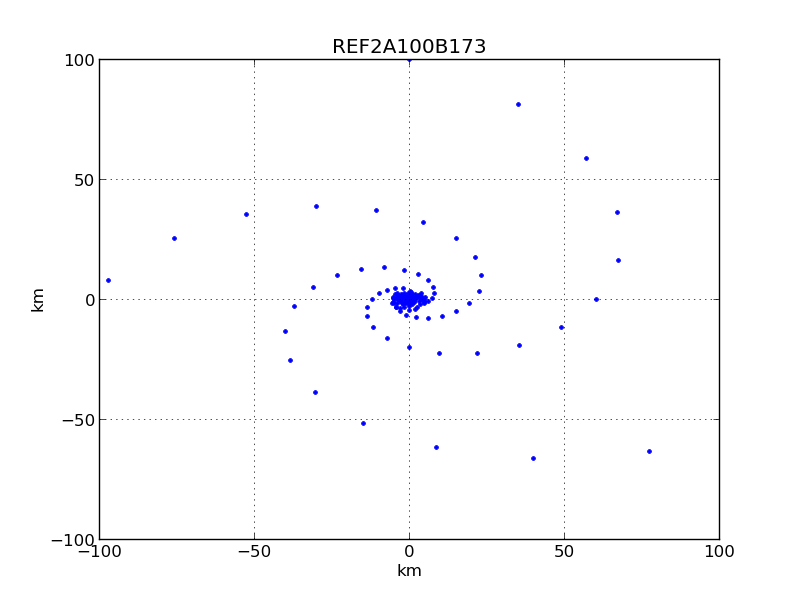
\includegraphics[width=0.300000\textwidth,trim= 0 .05cm 0 0.05cm]{{images/lay_SKA1REF2}.png} &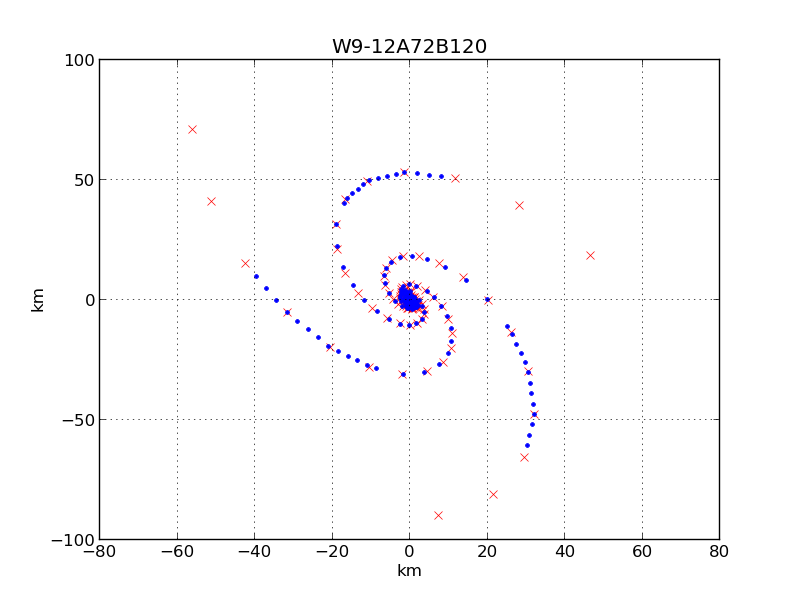
\includegraphics[width=0.300000\textwidth,trim= 0 .05cm 0 0.05cm]{{images/lay_SKA1W9-12A72B120}.png} &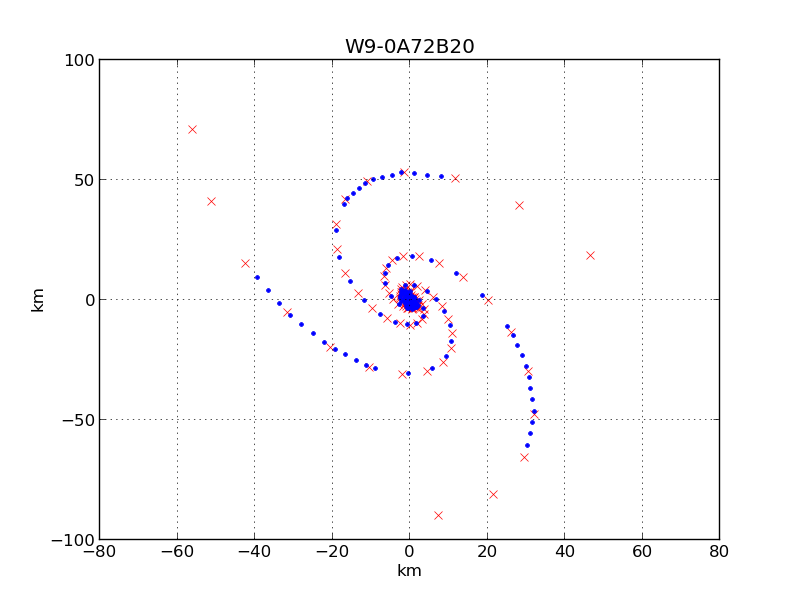
\includegraphics[width=0.300000\textwidth,trim= 0 .05cm 0 0.05cm]{{images/lay_SKA1W9-0A72B120}.png} 
 \\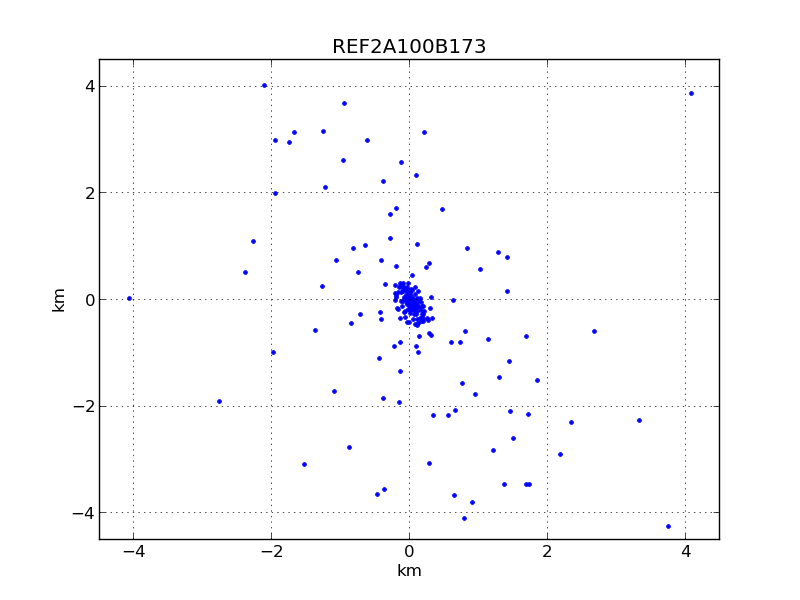
\includegraphics[width=0.300000\textwidth,trim= 0 .05cm 0 0.05cm]{{images/outer_core_SKA1REF2}.png} &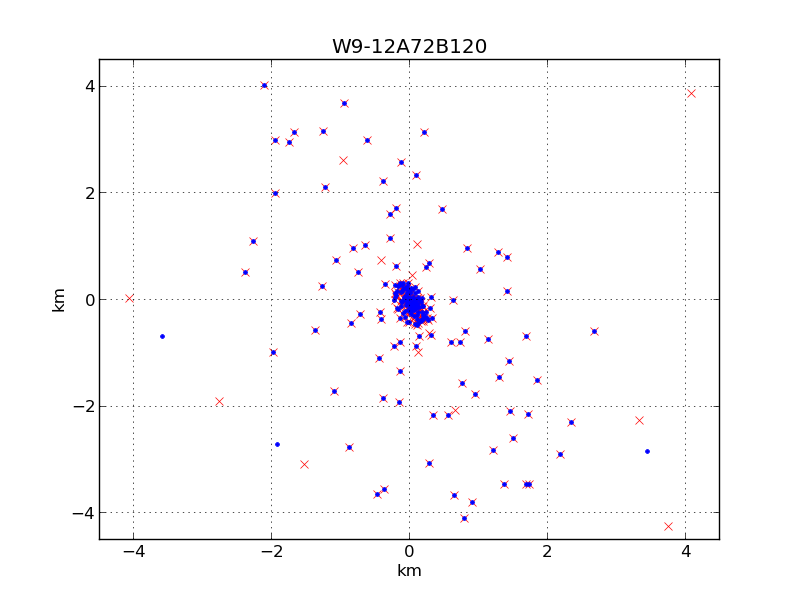
\includegraphics[width=0.300000\textwidth,trim= 0 .05cm 0 0.05cm]{{images/outer_core_SKA1W9-12A72B120}.png} &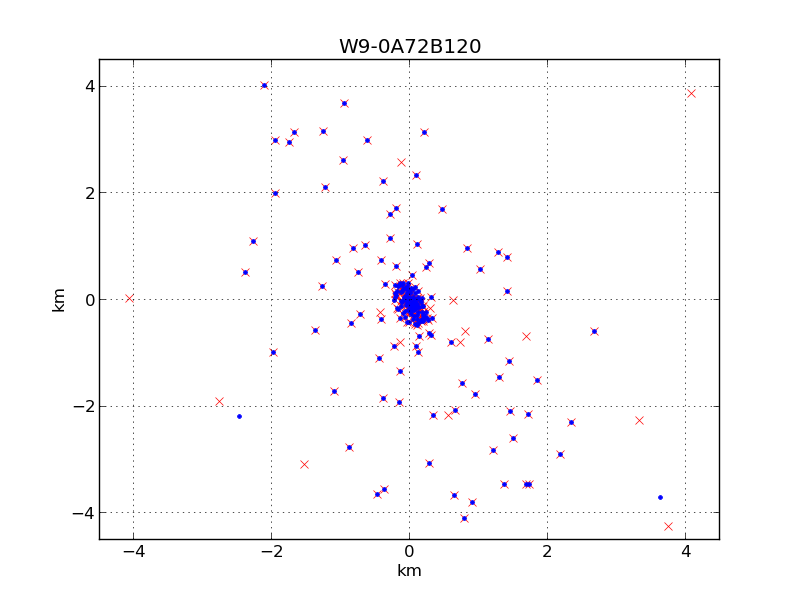
\includegraphics[width=0.300000\textwidth,trim= 0 .05cm 0 0.05cm]{{images/outer_core_SKA1W9-0A72B120}.png} 
 \\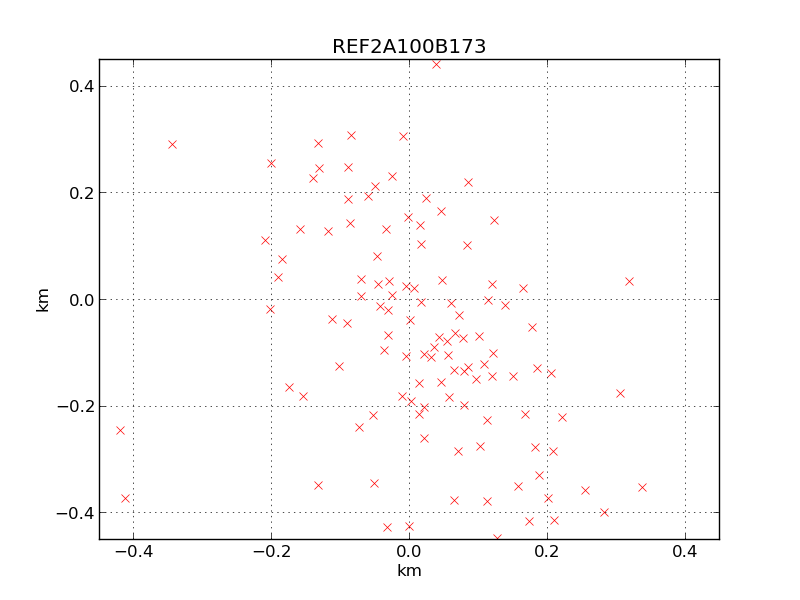
\includegraphics[width=0.300000\textwidth,trim= 0 .05cm 0 0.05cm]{{images/core_SKA1REF2}.png} &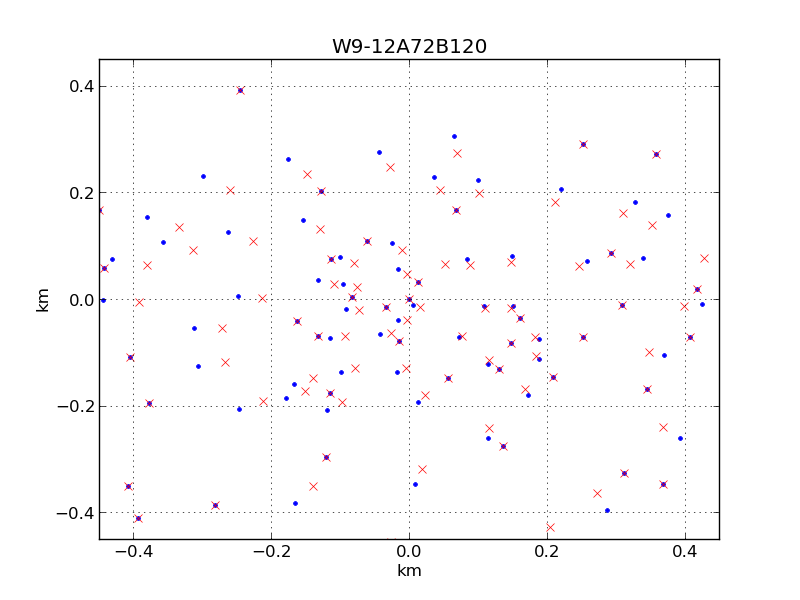
\includegraphics[width=0.300000\textwidth,trim= 0 .05cm 0 0.05cm]{{images/core_SKA1W9-12A72B120}.png} &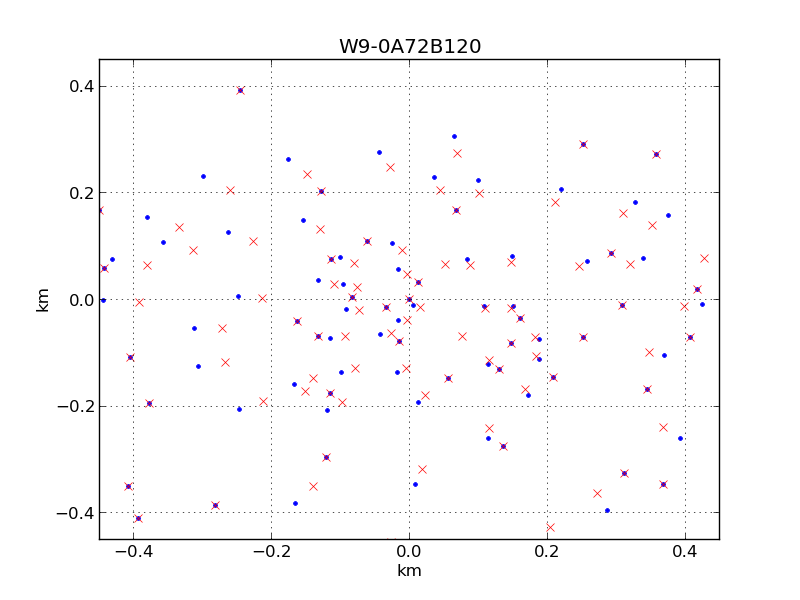
\includegraphics[width=0.300000\textwidth,trim= 0 .05cm 0 0.05cm]{{images/core_SKA1W9-0A72B120}.png} 
 \\\end{tabular}}
 \caption{Antenna layouts, REF2 plotted as a reference (red crosses)}\label{fig:lay}
\end{figure}
% baseline distribution histograms
\begin{figure}[H]
 \tiny{%%% autogen
 \begin{tabular}{ccc}
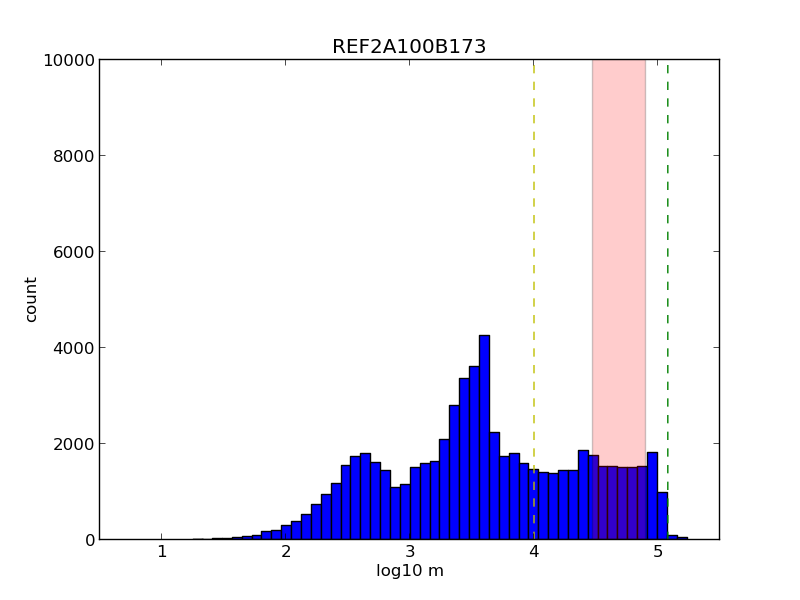
\includegraphics[width=0.300000\textwidth,trim= 0 .05cm 0 0.05cm]{{images/hist_SKA1REF2}.png} &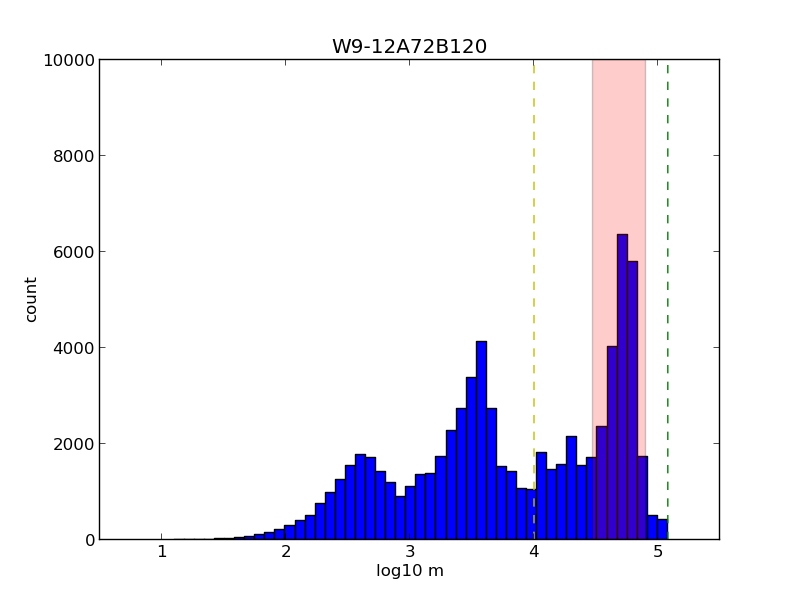
\includegraphics[width=0.300000\textwidth,trim= 0 .05cm 0 0.05cm]{{images/hist_SKA1W9-12A72B120}.png} &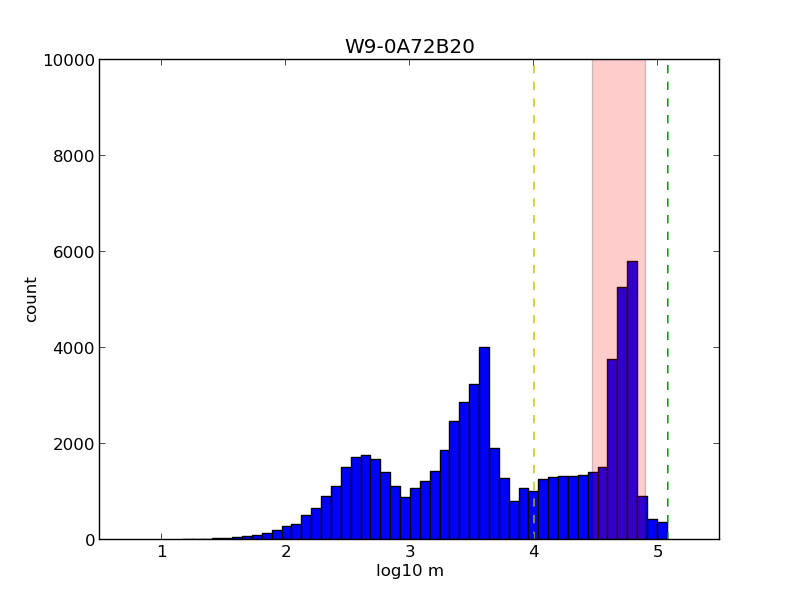
\includegraphics[width=0.300000\textwidth,trim= 0 .05cm 0 0.05cm]{{images/hist_SKA1W9-0A72B120}.png} 
 \\\end{tabular}}
 \caption{Baseline distribution with the uv-distance in $log_{10}$ km . Yellow and green dashed lines mark 10 and 120
kilometres respectively, and the pink strip represents baselines from 30-80km.}\label{fig:hist}
\end{figure}
\begin{figure}[H]
 \centering
 %%% autogen
 \begin{tabular}{ccc}
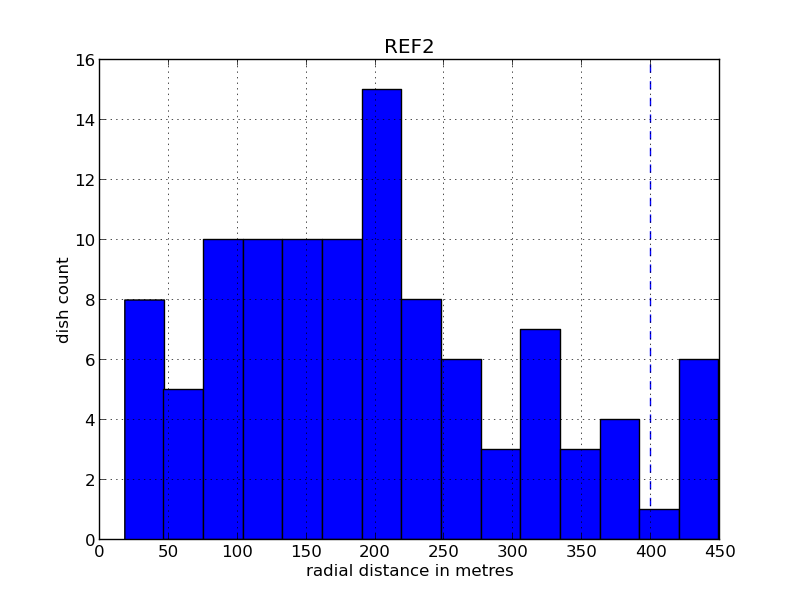
\includegraphics[width=0.300000\textwidth,trim= 0 .05cm 0 0.05cm]{{images/dish_hist-REF2}.png} &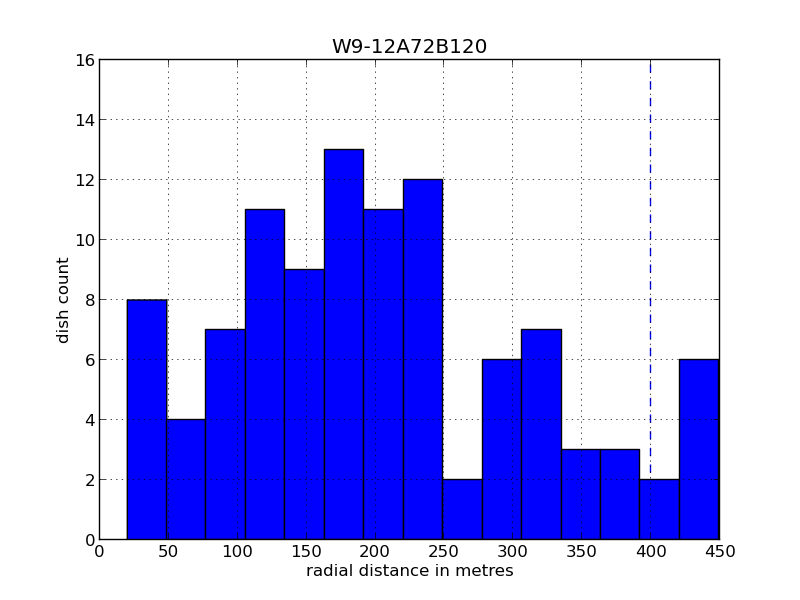
\includegraphics[width=0.300000\textwidth,trim= 0 .05cm 0 0.05cm]{{images/dish_hist-W9-12A72B120}.png} & 
 \\ \end{tabular}
 \caption{Dish density histograms (row 1) of the core for the layouts under consideration. The dashed line marks 400m. The core of
the W-9-12 layouts is the same, therefore we only need to plot one of these.}
\end{figure}
\begin{figure}[H]
 \centering
 %%% autogen
 \begin{tabular}{ccc}
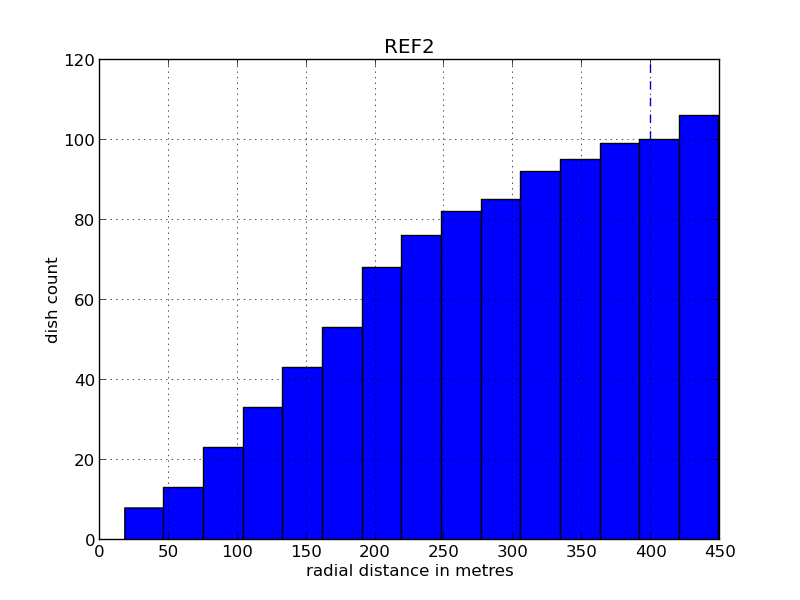
\includegraphics[width=0.300000\textwidth,trim= 0 .05cm 0 0.05cm]{{images/dish_cumhist-REF2}.png} &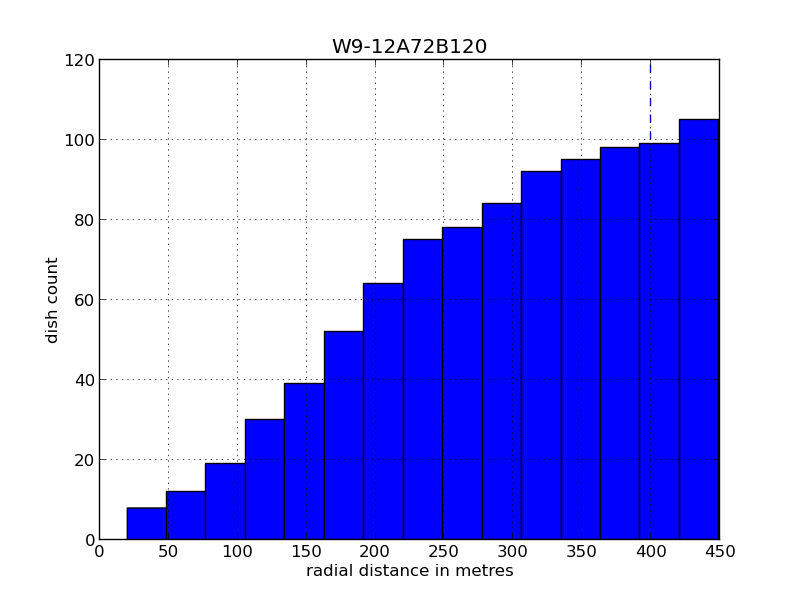
\includegraphics[width=0.300000\textwidth,trim= 0 .05cm 0 0.05cm]{{images/dish_cumhist-W9-12A72B120}.png} & 
 \\ \end{tabular}
 \caption{Cummulative dish density histograms (row 1) of the core for the layouts under consideration. The dashed line marks 400m.
The core of the W-9-12 layouts is the same, therefore we only need to plot one of these.}
\end{figure}
% uv-coverage plots 
\begin{figure}[H]
 \tiny{%%% autogen
 \begin{tabular}{ccc}
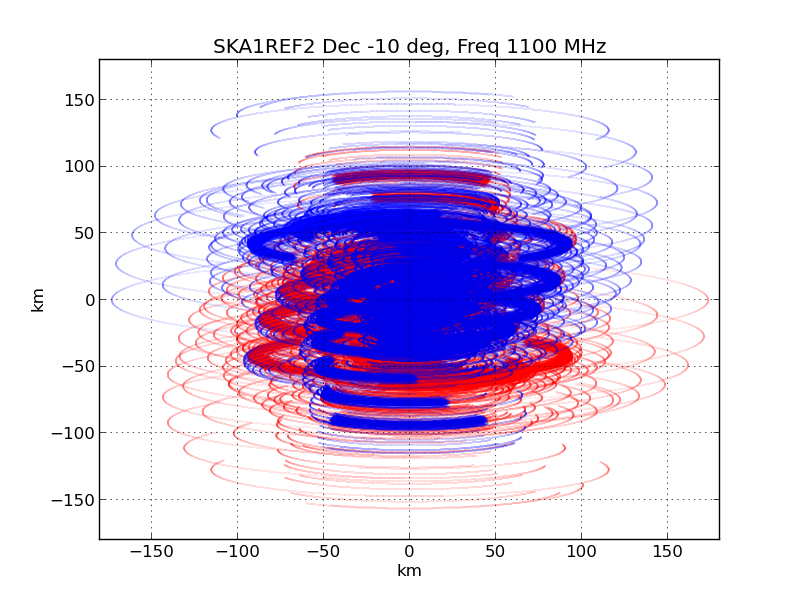
\includegraphics[width=0.300000\textwidth,trim= 0 .05cm 0 0.05cm]{{images/uvcov_SKA1REF2_-10_1100}.png} &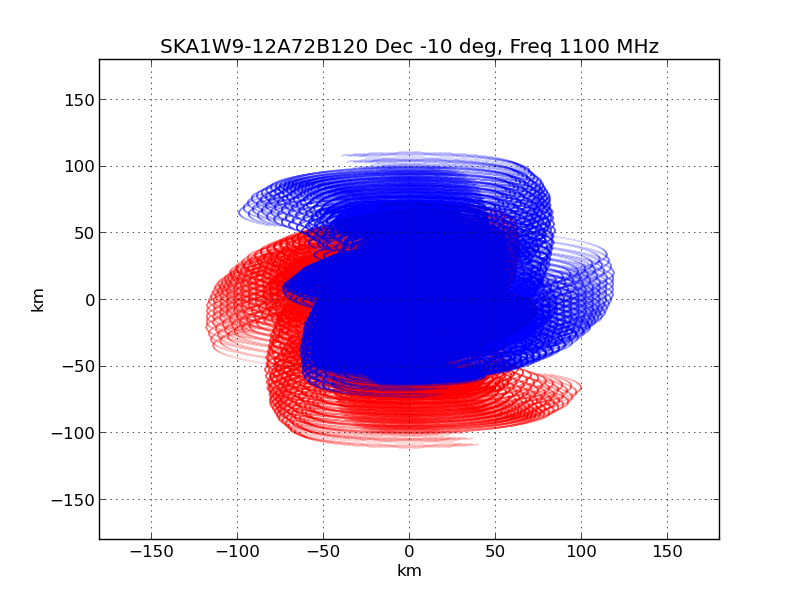
\includegraphics[width=0.300000\textwidth,trim= 0 .05cm 0 0.05cm]{{images/uvcov_SKA1W9-12A72B120_-10_1100}.png} &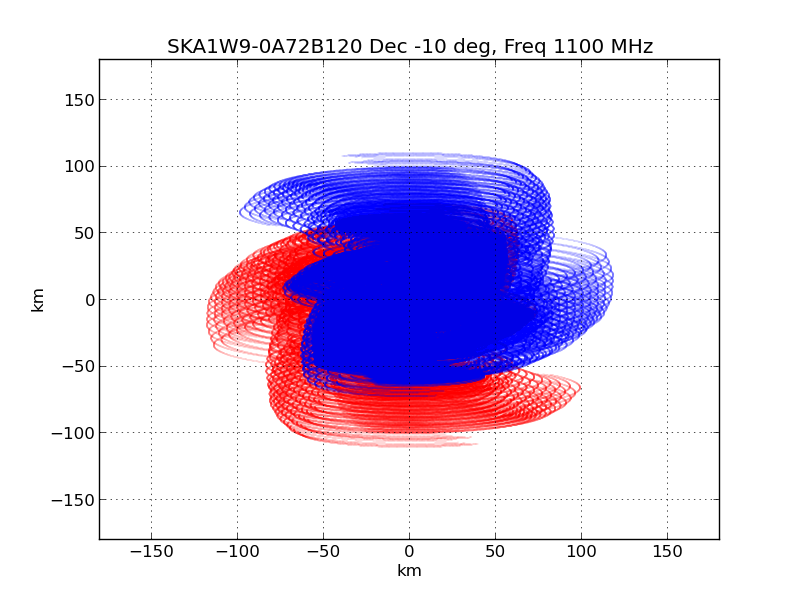
\includegraphics[width=0.300000\textwidth,trim= 0 .05cm 0 0.05cm]{{images/uvcov_SKA1W9-0A72B120_-10_1100}.png} 
 \\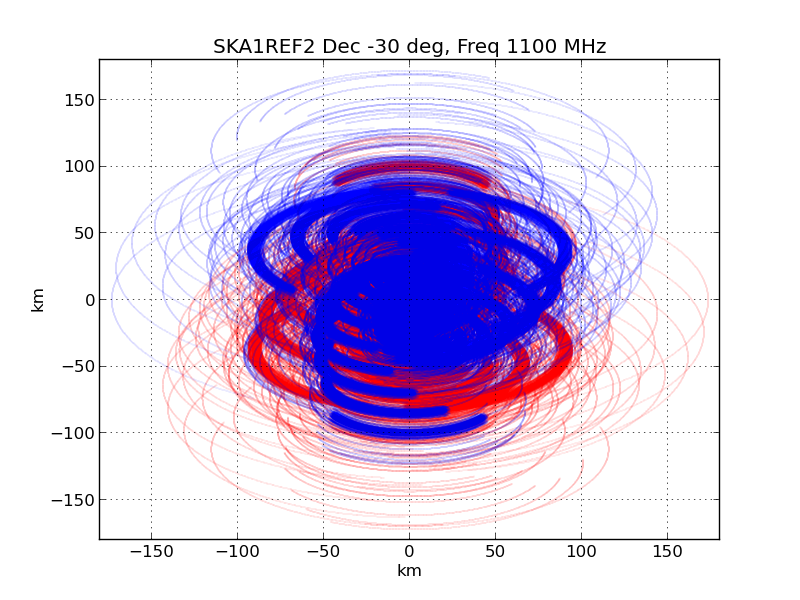
\includegraphics[width=0.300000\textwidth,trim= 0 .05cm 0 0.05cm]{{images/uvcov_SKA1REF2_-30_1100}.png} &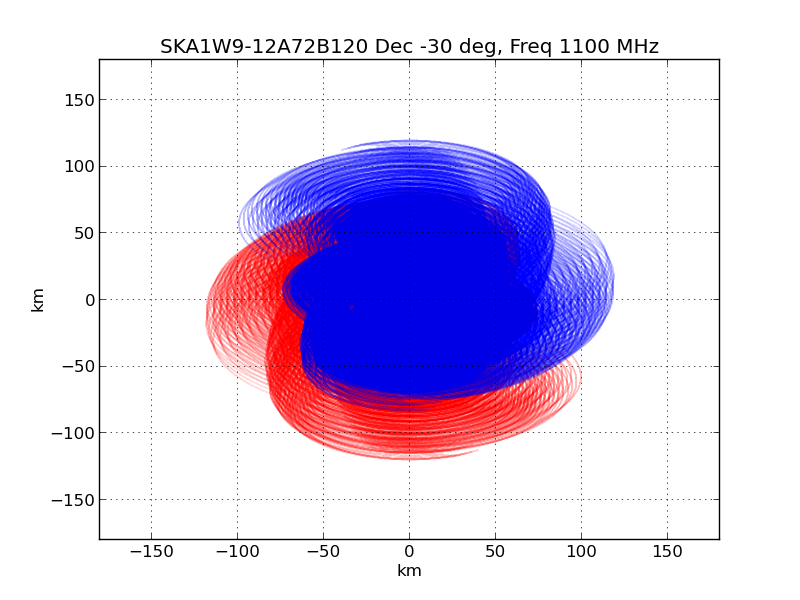
\includegraphics[width=0.300000\textwidth,trim= 0 .05cm 0 0.05cm]{{images/uvcov_SKA1W9-12A72B120_-30_1100}.png} &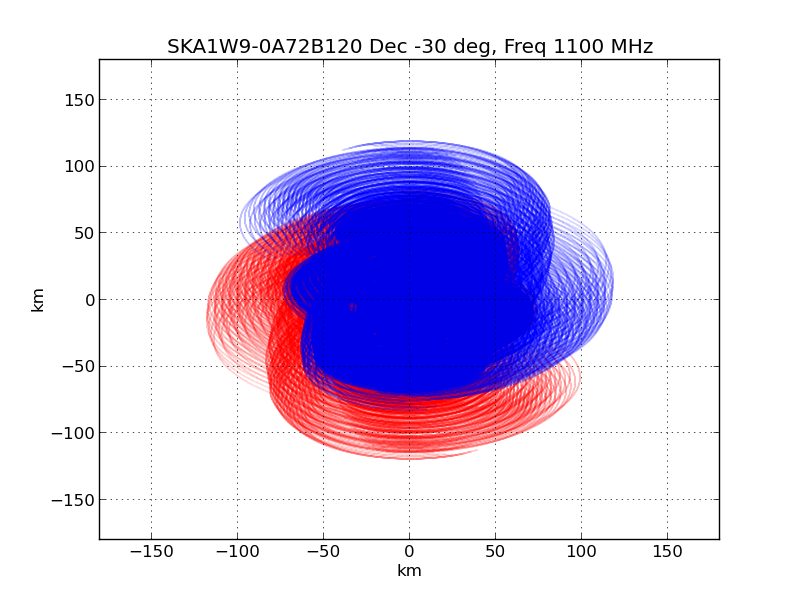
\includegraphics[width=0.300000\textwidth,trim= 0 .05cm 0 0.05cm]{{images/uvcov_SKA1W9-0A72B120_-30_1100}.png} 
 \\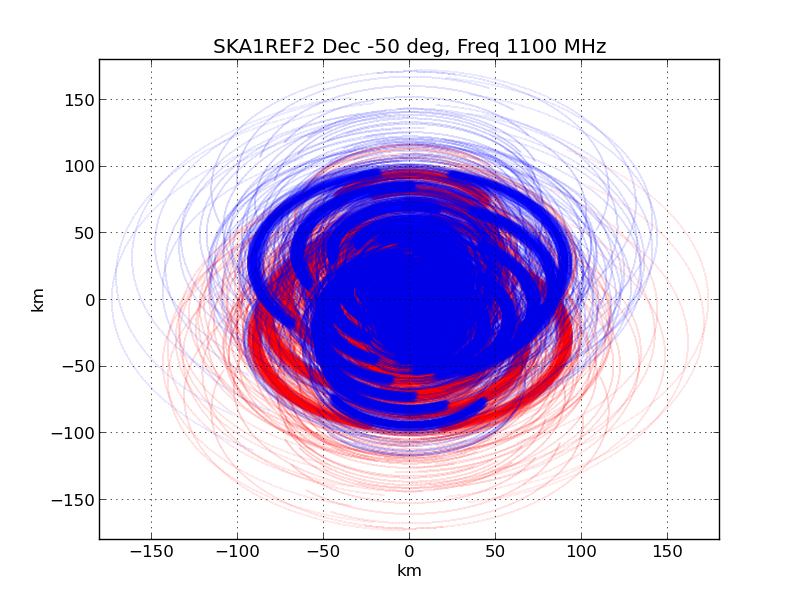
\includegraphics[width=0.300000\textwidth,trim= 0 .05cm 0 0.05cm]{{images/uvcov_SKA1REF2_-50_1100}.png} &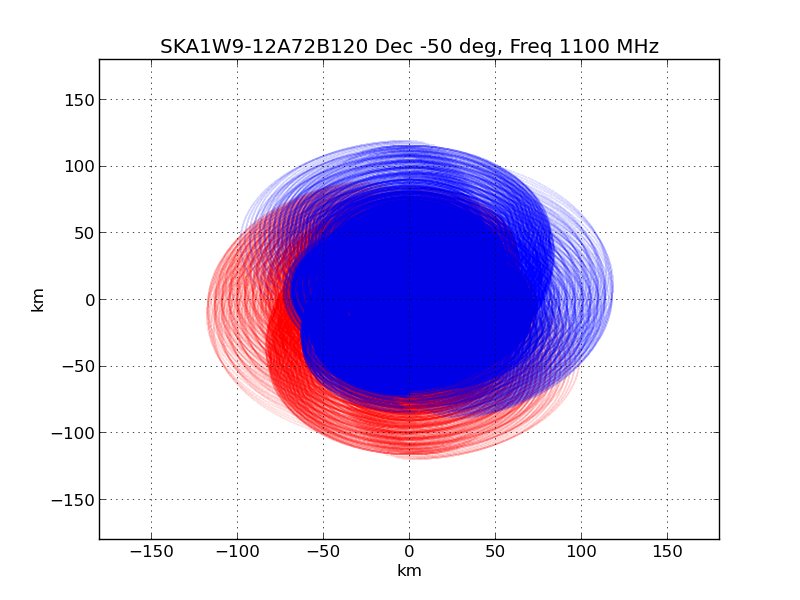
\includegraphics[width=0.300000\textwidth,trim= 0 .05cm 0 0.05cm]{{images/uvcov_SKA1W9-12A72B120_-50_1100}.png} &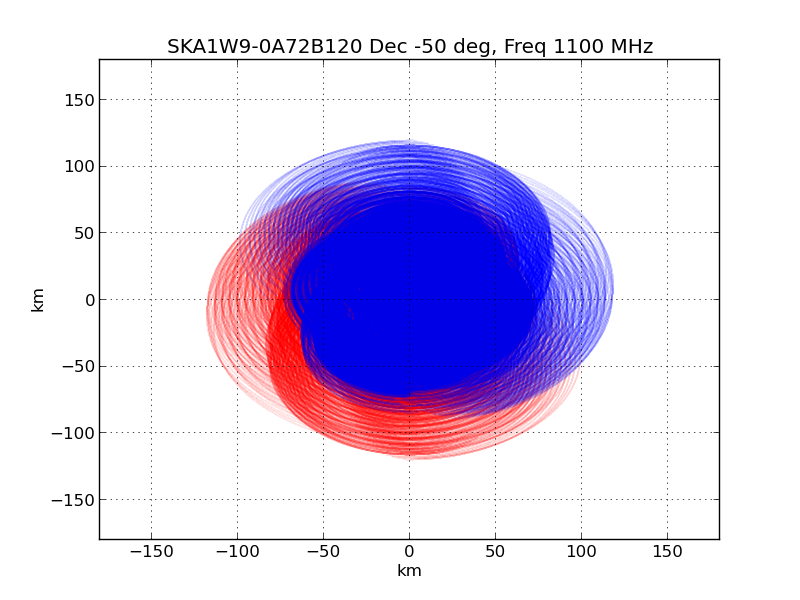
\includegraphics[width=0.300000\textwidth,trim= 0 .05cm 0 0.05cm]{{images/uvcov_SKA1W9-0A72B120_-50_1100}.png} 
 \\\end{tabular}}
 \caption{UV-Coverage for 8-hr tracks at 1.1 GHz (50MHz bandwidth) at declinations -50,-30,-10 for the different layouts. Blue
indicates uv-points, red indicates conjugate uv-points.}\label{fig:uvcov}
\end{figure}

\section{The Experiment}\label{sec:exp}
Our aim is to investigate the scale-dependent sensitivity of the layouts described in the previous section.
We use the \texttt{makems} tool to make simulated measurement sets (MS) of 8hr tracks with a 60s integration time for declinations
\{-50, -30, -10\} degrees at frequencies of \{650, 800, 1100\}MHz with a single 50MHz channel. The expected rms noise per real
and imaginary part for each visibility is calculated as 
\begin{equation}
\sigma_{\text{vis}} = \frac{\text{SEFD}}{\sqrt{2\Delta t\Delta \nu}}.
\end{equation}
We use the baseline designs SEFD value of 400 corresponding to the 15 m dishes. We then fill the MS with random Gaussian noise
using the computed value of the noise for a given integration and bandwidth. We then use the (CASA-derived) \texttt{lwimager} tool
to make maps of the PSF as well as dirty maps of the noise using various weighting schemes. Note that for uniform and robust
weighting, a crucial parameter is the size of the uv-bin over which weights are “uniformized”. By default this is determined from
the full image size, but \texttt{lwimager} allows one to uniformize the weights over bins corresponding to a user-defined FoV
instead. For these simulations uv-bins corresponding to a FoV of 10 arcmin were used. The following metrics were generated:\\ {\bf
Note:} These metrics are generated at different angular scales, this is done by applying an inner-taper\footnote{The weights for
the taper are generated using a Butterworth function.} to taper out baselines that do not fall within a given resolution range,
i.e., we only consider uv-points that correspond to a given resolution.
\begin{itemize}
 \item PSF full width at halfW maximum (FWHM) size (mean of the FWHM dimensions). This was measured by making high-resolution
images of the PSF (0.05 arcsec
resolution), and fitting a Gaussian to the PSF. Note that for the highly non-Gaussian PSFs corresponding to natural and (some)
robust weighting schemes, the fit is very poor, so the size parameter becomes somewhat ill-defined (Table \ref{tab:psf_mean}).
A catalog of PSF cross-sections is provided in Appendix \ref{app:psf}

 \item PSF symmetry (PSF size parameters are obtained as explained above). As a measure of PSF symmetry, we define 
$\text{PSF}_{sym}=1-\text{FWHM}_{min}/\text{FWHM}_{maj}$, then $\text{PSF}_{sym} = 0$ is perfect symmetry, and the symmetry
degenerates as $\text{PSF}_{sym}\,\,\, \rightarrow\,\,1$ (Table \ref{tab:psf_sym}).

 \item Rms pixel noise at different angular scales for 50kHz, 50MHz and 166MHz wide bands (Tables \ref{tab:noise50k} and
\ref{tab:noise166}).
 
 \item SNR for a 10$\mu$Jy source at 1100MHz with a spectral index of -0.7 after 8hrs for a 166MHz band (Table \ref{tab:snr10}).
 \item Average SNR over frequencies 650, 800 and 1100MHz (166MHz band)
   after 8 hours, for a 10$\mu$Jy source at 1100MHz
with a spectral index of -0.7 (Table \ref{tab:snravg}). {$\overline{SNR10}=\sqrt{SNR10_{650}^2 + SNR10_{800}^2 +
SNR10_{1100}^2}$}.
 \item Hours required to reach a mean SNR of 10 (Table \ref{tab:hours}).
\end{itemize}
% \section{Results}\label{sec:results}
%===========================================================Performance Stats===============================================
% Auto generated table
 \begin{table}[!htp]
 \tiny{
\subfloat[DEC=-10, natural weighting]{\begin{tabular}{|lccccc||ccccc||ccccc|} 
 \tabularnewline \cline{2-16} \multicolumn{1}{c}{ } & \multicolumn{5}{|c}{650MHz}  & \multicolumn{5}{c}{800MHz}  & \multicolumn{5}{c|}{1100MHz} \tabularnewline \cline{1-16} 
 resbin  &1 & 2 & 3 & 4 & 5 & 1 & 2 & 3 & 4 & 5 & 1 & 2 & 3 & 4 & 5 \tabularnewline \hline
SKA1REF2 & 0.65 \cellcolor{blue!18.00} & 1.33 \cellcolor{red!28.35} & 2.33 \cellcolor{green!18.00} & 3.35 \cellcolor{orange!18.68} & 803.1 \cellcolor{purple!19.31} & 0.60 \cellcolor{blue!18.00} & 1.33 \cellcolor{red!23.61} & 2.35 \cellcolor{green!18.19} & 3.34 \cellcolor{orange!20.44} & 792.3 \cellcolor{purple!18.58} & 0.59 \cellcolor{blue!21.07} & 1.33 \cellcolor{red!18.66} & 2.35 \cellcolor{green!20.87} & 3.35 \cellcolor{orange!20.00} & 763.6 \cellcolor{purple!19.11}\\ \hline 
SKA1W9-12A72B120 & 0.78 \cellcolor{blue!28.42} & 1.22 \cellcolor{red!19.02} & 2.35 \cellcolor{green!18.74} & 3.35 \cellcolor{orange!18.00} & 798.7 \cellcolor{purple!18.00} & 0.70 \cellcolor{blue!28.80} & 1.28 \cellcolor{red!18.40} & 2.35 \cellcolor{green!18.00} & 3.32 \cellcolor{orange!18.38} & 790.4 \cellcolor{purple!18.00} & 0.57 \cellcolor{blue!18.40} & 1.32 \cellcolor{red!18.00} & 2.32 \cellcolor{green!18.00} & 3.33 \cellcolor{orange!18.00} & 763.3 \cellcolor{purple!18.00}\\ \hline 
SKA1W9-0A72B120 & 0.78 \cellcolor{blue!28.75} & 1.21 \cellcolor{red!18.00} & 2.35 \cellcolor{green!18.66} & 3.35 \cellcolor{orange!18.14} & 802.2 \cellcolor{purple!19.04} & 0.70 \cellcolor{blue!28.98} & 1.27 \cellcolor{red!18.00} & 2.36 \cellcolor{green!18.74} & 3.31 \cellcolor{orange!18.00} & 796.6 \cellcolor{purple!19.88} & 0.56 \cellcolor{blue!18.00} & 1.32 \cellcolor{red!18.27} & 2.34 \cellcolor{green!19.67} & 3.37 \cellcolor{orange!21.90} & 773.3 \cellcolor{purple!50.99}\\ \hline 
SKASUR & 1.17 \cellcolor{blue!60.00} & 1.69 \cellcolor{red!60.00} & 3.09 \cellcolor{green!60.00} & 3.88 \cellcolor{orange!60.00} & 938.3 \cellcolor{purple!60.00} & 1.00 \cellcolor{blue!60.00} & 1.69 \cellcolor{red!60.00} & 2.81 \cellcolor{green!60.00} & 3.78 \cellcolor{orange!60.00} & 930.5 \cellcolor{purple!60.00} & 0.86 \cellcolor{blue!60.00} & 1.80 \cellcolor{red!60.00} & 2.71 \cellcolor{green!60.00} & 3.75 \cellcolor{orange!60.00} & 776 \cellcolor{purple!60.00}\tabularnewline \hline 
\end{tabular}}\hfil 
\subfloat[DEC=-10, robust-2 weighting ]{\begin{tabular}{|lccccc||ccccc||ccccc|} 
 \tabularnewline \cline{2-16} \multicolumn{1}{c}{ } & \multicolumn{5}{|c}{650MHz}  & \multicolumn{5}{c}{800MHz}  & \multicolumn{5}{c|}{1100MHz} \tabularnewline \cline{1-16} 
 resbin  &1 & 2 & 3 & 4 & 5 & 1 & 2 & 3 & 4 & 5 & 1 & 2 & 3 & 4 & 5 \tabularnewline \hline
SKA1REF2 & 0.73 \cellcolor{blue!18.00} & 1.22 \cellcolor{red!22.54} & 2.25 \cellcolor{green!18.58} & 3.26 \cellcolor{orange!19.10} & 745.2 \cellcolor{purple!20.22} & 0.62 \cellcolor{blue!18.00} & 1.21 \cellcolor{red!23.22} & 2.24 \cellcolor{green!18.71} & 3.25 \cellcolor{orange!19.18} & 791.8 \cellcolor{purple!18.46} & 0.53 \cellcolor{blue!18.00} & 1.19 \cellcolor{red!20.19} & 2.24 \cellcolor{green!19.76} & 3.26 \cellcolor{orange!26.56} & 761.5 \cellcolor{purple!18.00}\\ \hline 
SKA1W9-12A72B120 & 0.77 \cellcolor{blue!20.06} & 1.16 \cellcolor{red!18.07} & 2.24 \cellcolor{green!18.00} & 3.25 \cellcolor{orange!18.00} & 736 \cellcolor{purple!18.00} & 0.64 \cellcolor{blue!19.56} & 1.15 \cellcolor{red!18.02} & 2.24 \cellcolor{green!18.00} & 3.25 \cellcolor{orange!18.00} & 790.2 \cellcolor{purple!18.00} & 0.53 \cellcolor{blue!18.61} & 1.17 \cellcolor{red!18.00} & 2.23 \cellcolor{green!18.00} & 3.25 \cellcolor{orange!18.00} & 761.8 \cellcolor{purple!18.84}\\ \hline 
SKA1W9-0A72B120 & 0.79 \cellcolor{blue!20.78} & 1.16 \cellcolor{red!18.00} & 2.25 \cellcolor{green!18.47} & 3.25 \cellcolor{orange!18.01} & 739.2 \cellcolor{purple!18.76} & 0.65 \cellcolor{blue!20.35} & 1.15 \cellcolor{red!18.00} & 2.24 \cellcolor{green!18.62} & 3.25 \cellcolor{orange!18.54} & 796.2 \cellcolor{purple!19.66} & 0.54 \cellcolor{blue!19.35} & 1.17 \cellcolor{red!18.71} & 2.24 \cellcolor{green!19.83} & 3.25 \cellcolor{orange!24.33} & 771.7 \cellcolor{purple!47.43}\\ \hline 
SKASUR & 1.59 \cellcolor{blue!60.00} & 1.75 \cellcolor{red!60.00} & 2.99 \cellcolor{green!60.00} & 3.57 \cellcolor{orange!60.00} & 910.2 \cellcolor{purple!60.00} & 1.32 \cellcolor{blue!60.00} & 1.62 \cellcolor{red!60.00} & 2.71 \cellcolor{green!60.00} & 3.43 \cellcolor{orange!60.00} & 942.1 \cellcolor{purple!60.00} & 1.00 \cellcolor{blue!60.00} & 1.60 \cellcolor{red!60.00} & 2.41 \cellcolor{green!60.00} & 3.29 \cellcolor{orange!60.00} & 776 \cellcolor{purple!60.00}\tabularnewline \hline 
\end{tabular}}\hfil 
\subfloat[DEC=-10, robust-2 weighting with a 1 arcsec Gaussian taper]{\begin{tabular}{|lccccc||ccccc||ccccc|} 
 \tabularnewline \cline{2-16} \multicolumn{1}{c}{ } & \multicolumn{5}{|c}{650MHz}  & \multicolumn{5}{c}{800MHz}  & \multicolumn{5}{c|}{1100MHz} \tabularnewline \cline{1-16} 
 resbin  &1 & 2 & 3 & 4 & 5 & 1 & 2 & 3 & 4 & 5 & 1 & 2 & 3 & 4 & 5 \tabularnewline \hline
SKA1REF2 & 1.03 \cellcolor{blue!19.09} & 1.33 \cellcolor{red!22.77} & 2.27 \cellcolor{green!18.56} & 3.27 \cellcolor{orange!19.09} & 745.2 \cellcolor{purple!20.22} & 0.98 \cellcolor{blue!21.10} & 1.31 \cellcolor{red!22.78} & 2.27 \cellcolor{green!18.73} & 3.26 \cellcolor{orange!19.19} & 791.8 \cellcolor{purple!18.46} & 0.94 \cellcolor{blue!22.90} & 1.29 \cellcolor{red!20.03} & 2.26 \cellcolor{green!19.77} & 3.26 \cellcolor{orange!26.60} & 761.5 \cellcolor{purple!18.00}\\ \hline 
SKA1W9-12A72B120 & 1.01 \cellcolor{blue!18.00} & 1.26 \cellcolor{red!18.15} & 2.26 \cellcolor{green!18.00} & 3.26 \cellcolor{orange!18.00} & 736 \cellcolor{purple!18.00} & 0.93 \cellcolor{blue!18.00} & 1.25 \cellcolor{red!18.02} & 2.26 \cellcolor{green!18.00} & 3.26 \cellcolor{orange!18.00} & 790.2 \cellcolor{purple!18.00} & 0.87 \cellcolor{blue!18.07} & 1.26 \cellcolor{red!18.00} & 2.25 \cellcolor{green!18.00} & 3.26 \cellcolor{orange!18.00} & 761.8 \cellcolor{purple!18.84}\\ \hline 
SKA1W9-0A72B120 & 1.02 \cellcolor{blue!18.28} & 1.25 \cellcolor{red!18.00} & 2.27 \cellcolor{green!18.45} & 3.26 \cellcolor{orange!18.00} & 739.2 \cellcolor{purple!18.76} & 0.94 \cellcolor{blue!18.12} & 1.25 \cellcolor{red!18.00} & 2.26 \cellcolor{green!18.60} & 3.26 \cellcolor{orange!18.50} & 796.2 \cellcolor{purple!19.66} & 0.87 \cellcolor{blue!18.00} & 1.27 \cellcolor{red!18.58} & 2.26 \cellcolor{green!19.67} & 3.26 \cellcolor{orange!24.48} & 771.7 \cellcolor{purple!47.43}\\ \hline 
SKASUR & 1.83 \cellcolor{blue!60.00} & 1.88 \cellcolor{red!60.00} & 3.00 \cellcolor{green!60.00} & 3.57 \cellcolor{orange!60.00} & 910.2 \cellcolor{purple!60.00} & 1.61 \cellcolor{blue!60.00} & 1.77 \cellcolor{red!60.00} & 2.73 \cellcolor{green!60.00} & 3.43 \cellcolor{orange!60.00} & 942.1 \cellcolor{purple!60.00} & 1.41 \cellcolor{blue!60.00} & 1.74 \cellcolor{red!60.00} & 2.43 \cellcolor{green!60.00} & 3.29 \cellcolor{orange!60.00} & 776 \cellcolor{purple!60.00}\tabularnewline \hline 
\end{tabular}}\hfil 
\subfloat[DEC=-30, natural weighting]{\begin{tabular}{|lccccc||ccccc||ccccc|} 
 \tabularnewline \cline{2-16} \multicolumn{1}{c}{ } & \multicolumn{5}{|c}{650MHz}  & \multicolumn{5}{c}{800MHz}  & \multicolumn{5}{c|}{1100MHz} \tabularnewline \cline{1-16} 
 resbin  &1 & 2 & 3 & 4 & 5 & 1 & 2 & 3 & 4 & 5 & 1 & 2 & 3 & 4 & 5 \tabularnewline \hline
SKA1REF2 & 0.65 \cellcolor{blue!18.00} & 1.34 \cellcolor{red!29.33} & 2.35 \cellcolor{green!18.00} & 3.37 \cellcolor{orange!20.22} & 797.3 \cellcolor{purple!19.01} & 0.60 \cellcolor{blue!18.00} & 1.33 \cellcolor{red!23.33} & 2.35 \cellcolor{green!19.11} & 3.34 \cellcolor{orange!21.22} & 790.6 \cellcolor{purple!18.09} & 0.59 \cellcolor{blue!22.62} & 1.33 \cellcolor{red!18.00} & 2.35 \cellcolor{green!21.26} & 3.35 \cellcolor{orange!18.52} & 759.2 \cellcolor{purple!38.11}\\ \hline 
SKA1W9-12A72B120 & 0.78 \cellcolor{blue!28.32} & 1.22 \cellcolor{red!19.15} & 2.37 \cellcolor{green!19.18} & 3.35 \cellcolor{orange!18.86} & 792.9 \cellcolor{purple!18.00} & 0.69 \cellcolor{blue!27.25} & 1.29 \cellcolor{red!18.21} & 2.34 \cellcolor{green!18.00} & 3.31 \cellcolor{orange!18.65} & 790.2 \cellcolor{purple!18.00} & 0.56 \cellcolor{blue!18.49} & 1.33 \cellcolor{red!18.00} & 2.32 \cellcolor{green!18.00} & 3.34 \cellcolor{orange!18.00} & 752.2 \cellcolor{purple!18.00}\\ \hline 
SKA1W9-0A72B120 & 0.79 \cellcolor{blue!28.64} & 1.21 \cellcolor{red!18.00} & 2.35 \cellcolor{green!18.24} & 3.34 \cellcolor{orange!18.00} & 798.1 \cellcolor{purple!19.19} & 0.70 \cellcolor{blue!27.34} & 1.29 \cellcolor{red!18.00} & 2.35 \cellcolor{green!18.96} & 3.30 \cellcolor{orange!18.00} & 795.5 \cellcolor{purple!19.31} & 0.55 \cellcolor{blue!18.00} & 1.34 \cellcolor{red!18.66} & 2.33 \cellcolor{green!19.55} & 3.37 \cellcolor{orange!20.52} & 763.4 \cellcolor{purple!50.06}\\ \hline 
SKASUR & 1.20 \cellcolor{blue!60.00} & 1.68 \cellcolor{red!60.00} & 3.12 \cellcolor{green!60.00} & 3.92 \cellcolor{orange!60.00} & 976.6 \cellcolor{purple!60.00} & 1.04 \cellcolor{blue!60.00} & 1.62 \cellcolor{red!60.00} & 2.87 \cellcolor{green!60.00} & 3.81 \cellcolor{orange!60.00} & 961 \cellcolor{purple!60.00} & 0.87 \cellcolor{blue!60.00} & 1.75 \cellcolor{red!60.00} & 2.75 \cellcolor{green!60.00} & 3.77 \cellcolor{orange!60.00} & 766.8 \cellcolor{purple!60.00}\tabularnewline \hline 
\end{tabular}}\hfil 
\subfloat[DEC=-30, robust-2 weighting ]{\begin{tabular}{|lccccc||ccccc||ccccc|} 
 \tabularnewline \cline{2-16} \multicolumn{1}{c}{ } & \multicolumn{5}{|c}{650MHz}  & \multicolumn{5}{c}{800MHz}  & \multicolumn{5}{c|}{1100MHz} \tabularnewline \cline{1-16} 
 resbin  &1 & 2 & 3 & 4 & 5 & 1 & 2 & 3 & 4 & 5 & 1 & 2 & 3 & 4 & 5 \tabularnewline \hline
SKA1REF2 & 0.71 \cellcolor{blue!18.00} & 1.21 \cellcolor{red!23.03} & 2.24 \cellcolor{green!18.12} & 3.26 \cellcolor{orange!19.27} & 737.5 \cellcolor{purple!18.83} & 0.60 \cellcolor{blue!18.00} & 1.19 \cellcolor{red!23.62} & 2.24 \cellcolor{green!19.42} & 3.24 \cellcolor{orange!19.33} & 789.8 \cellcolor{purple!18.00} & 0.51 \cellcolor{blue!18.00} & 1.18 \cellcolor{red!20.35} & 2.24 \cellcolor{green!22.22} & 3.25 \cellcolor{orange!18.00} & 757.1 \cellcolor{purple!40.65}\\ \hline 
SKA1W9-12A72B120 & 0.75 \cellcolor{blue!20.17} & 1.15 \cellcolor{red!18.13} & 2.24 \cellcolor{green!18.00} & 3.25 \cellcolor{orange!18.50} & 732.5 \cellcolor{purple!18.00} & 0.63 \cellcolor{blue!19.85} & 1.14 \cellcolor{red!18.00} & 2.23 \cellcolor{green!18.00} & 3.24 \cellcolor{orange!18.00} & 789.9 \cellcolor{purple!18.04} & 0.52 \cellcolor{blue!18.51} & 1.16 \cellcolor{red!18.00} & 2.22 \cellcolor{green!18.00} & 3.25 \cellcolor{orange!19.85} & 750.8 \cellcolor{purple!18.00}\\ \hline 
SKA1W9-0A72B120 & 0.77 \cellcolor{blue!20.93} & 1.15 \cellcolor{red!18.00} & 2.25 \cellcolor{green!18.89} & 3.25 \cellcolor{orange!18.00} & 737.9 \cellcolor{purple!18.89} & 0.64 \cellcolor{blue!20.65} & 1.14 \cellcolor{red!18.05} & 2.23 \cellcolor{green!18.27} & 3.25 \cellcolor{orange!22.37} & 795.2 \cellcolor{purple!19.35} & 0.53 \cellcolor{blue!19.17} & 1.17 \cellcolor{red!19.12} & 2.23 \cellcolor{green!20.87} & 3.25 \cellcolor{orange!26.54} & 762.5 \cellcolor{purple!60.00}\\ \hline 
SKASUR & 1.54 \cellcolor{blue!60.00} & 1.65 \cellcolor{red!60.00} & 2.71 \cellcolor{green!60.00} & 3.47 \cellcolor{orange!60.00} & 988.6 \cellcolor{purple!60.00} & 1.27 \cellcolor{blue!60.00} & 1.53 \cellcolor{red!60.00} & 2.57 \cellcolor{green!60.00} & 3.38 \cellcolor{orange!60.00} & 960.7 \cellcolor{purple!60.00} & 0.95 \cellcolor{blue!60.00} & 1.45 \cellcolor{red!60.00} & 2.36 \cellcolor{green!60.00} & 3.27 \cellcolor{orange!60.00} & 758.2 \cellcolor{purple!44.64}\tabularnewline \hline 
\end{tabular}}\hfil 
\subfloat[DEC=-30, robust-2 weighting with a 1 arcsec Gaussian taper]{\begin{tabular}{|lccccc||ccccc||ccccc|} 
 \tabularnewline \cline{2-16} \multicolumn{1}{c}{ } & \multicolumn{5}{|c}{650MHz}  & \multicolumn{5}{c}{800MHz}  & \multicolumn{5}{c|}{1100MHz} \tabularnewline \cline{1-16} 
 resbin  &1 & 2 & 3 & 4 & 5 & 1 & 2 & 3 & 4 & 5 & 1 & 2 & 3 & 4 & 5 \tabularnewline \hline
SKA1REF2 & 1.02 \cellcolor{blue!19.40} & 1.31 \cellcolor{red!23.21} & 2.26 \cellcolor{green!18.12} & 3.26 \cellcolor{orange!19.28} & 737.5 \cellcolor{purple!18.83} & 0.97 \cellcolor{blue!21.46} & 1.29 \cellcolor{red!23.11} & 2.27 \cellcolor{green!19.42} & 3.25 \cellcolor{orange!19.37} & 789.8 \cellcolor{purple!18.00} & 0.93 \cellcolor{blue!23.05} & 1.28 \cellcolor{red!20.13} & 2.26 \cellcolor{green!22.19} & 3.26 \cellcolor{orange!18.00} & 757.1 \cellcolor{purple!40.65}\\ \hline 
SKA1W9-12A72B120 & 1.00 \cellcolor{blue!18.00} & 1.25 \cellcolor{red!18.18} & 2.26 \cellcolor{green!18.00} & 3.26 \cellcolor{orange!18.50} & 732.5 \cellcolor{purple!18.00} & 0.92 \cellcolor{blue!18.00} & 1.24 \cellcolor{red!18.00} & 2.25 \cellcolor{green!18.00} & 3.25 \cellcolor{orange!18.00} & 789.9 \cellcolor{purple!18.04} & 0.87 \cellcolor{blue!18.04} & 1.26 \cellcolor{red!18.00} & 2.25 \cellcolor{green!18.00} & 3.26 \cellcolor{orange!20.14} & 750.8 \cellcolor{purple!18.00}\\ \hline 
SKA1W9-0A72B120 & 1.00 \cellcolor{blue!18.27} & 1.25 \cellcolor{red!18.00} & 2.27 \cellcolor{green!18.85} & 3.26 \cellcolor{orange!18.00} & 737.9 \cellcolor{purple!18.89} & 0.92 \cellcolor{blue!18.10} & 1.24 \cellcolor{red!18.10} & 2.26 \cellcolor{green!18.22} & 3.26 \cellcolor{orange!22.35} & 795.2 \cellcolor{purple!19.35} & 0.87 \cellcolor{blue!18.00} & 1.27 \cellcolor{red!18.90} & 2.26 \cellcolor{green!20.61} & 3.26 \cellcolor{orange!27.02} & 762.5 \cellcolor{purple!60.00}\\ \hline 
SKASUR & 1.74 \cellcolor{blue!60.00} & 1.77 \cellcolor{red!60.00} & 2.73 \cellcolor{green!60.00} & 3.47 \cellcolor{orange!60.00} & 988.6 \cellcolor{purple!60.00} & 1.53 \cellcolor{blue!60.00} & 1.65 \cellcolor{red!60.00} & 2.59 \cellcolor{green!60.00} & 3.38 \cellcolor{orange!60.00} & 960.7 \cellcolor{purple!60.00} & 1.32 \cellcolor{blue!60.00} & 1.59 \cellcolor{red!60.00} & 2.39 \cellcolor{green!60.00} & 3.28 \cellcolor{orange!60.00} & 758.2 \cellcolor{purple!44.64}\tabularnewline \hline 
\end{tabular}}\hfil 
\subfloat[DEC=-50, natural weighting]{\begin{tabular}{|lccccc||ccccc||ccccc|} 
 \tabularnewline \cline{2-16} \multicolumn{1}{c}{ } & \multicolumn{5}{|c}{650MHz}  & \multicolumn{5}{c}{800MHz}  & \multicolumn{5}{c|}{1100MHz} \tabularnewline \cline{1-16} 
 resbin  &1 & 2 & 3 & 4 & 5 & 1 & 2 & 3 & 4 & 5 & 1 & 2 & 3 & 4 & 5 \tabularnewline \hline
SKA1REF2 & 0.65 \cellcolor{blue!18.00} & 1.34 \cellcolor{red!30.72} & 2.34 \cellcolor{green!18.00} & 3.35 \cellcolor{orange!19.10} & 799.8 \cellcolor{purple!18.67} & 0.60 \cellcolor{blue!18.00} & 1.33 \cellcolor{red!26.18} & 2.36 \cellcolor{green!19.32} & 3.34 \cellcolor{orange!21.20} & 789.6 \cellcolor{purple!18.83} & 0.58 \cellcolor{blue!21.48} & 1.33 \cellcolor{red!18.59} & 2.34 \cellcolor{green!21.11} & 3.36 \cellcolor{orange!20.10} & 763.9 \cellcolor{purple!33.62}\\ \hline 
SKA1W9-12A72B120 & 0.79 \cellcolor{blue!26.96} & 1.22 \cellcolor{red!19.23} & 2.35 \cellcolor{green!18.82} & 3.34 \cellcolor{orange!18.00} & 796.7 \cellcolor{purple!18.00} & 0.70 \cellcolor{blue!27.28} & 1.28 \cellcolor{red!18.51} & 2.35 \cellcolor{green!18.00} & 3.32 \cellcolor{orange!18.00} & 786.4 \cellcolor{purple!18.00} & 0.56 \cellcolor{blue!18.43} & 1.33 \cellcolor{red!18.00} & 2.32 \cellcolor{green!18.00} & 3.34 \cellcolor{orange!18.00} & 756.6 \cellcolor{purple!18.00}\\ \hline 
SKA1W9-0A72B120 & 0.79 \cellcolor{blue!27.24} & 1.21 \cellcolor{red!18.00} & 2.34 \cellcolor{green!18.04} & 3.35 \cellcolor{orange!19.26} & 799.6 \cellcolor{purple!18.62} & 0.70 \cellcolor{blue!27.44} & 1.28 \cellcolor{red!18.00} & 2.35 \cellcolor{green!18.51} & 3.32 \cellcolor{orange!18.32} & 791 \cellcolor{purple!19.21} & 0.56 \cellcolor{blue!18.00} & 1.34 \cellcolor{red!19.39} & 2.33 \cellcolor{green!20.06} & 3.39 \cellcolor{orange!23.89} & 768.3 \cellcolor{purple!42.91}\\ \hline 
SKASUR & 1.28 \cellcolor{blue!60.00} & 1.63 \cellcolor{red!60.00} & 2.84 \cellcolor{green!60.00} & 3.78 \cellcolor{orange!60.00} & 995.7 \cellcolor{purple!60.00} & 1.06 \cellcolor{blue!60.00} & 1.53 \cellcolor{red!60.00} & 2.74 \cellcolor{green!60.00} & 3.69 \cellcolor{orange!60.00} & 946.1 \cellcolor{purple!60.00} & 0.87 \cellcolor{blue!60.00} & 1.54 \cellcolor{red!60.00} & 2.66 \cellcolor{green!60.00} & 3.68 \cellcolor{orange!60.00} & 776.2 \cellcolor{purple!60.00}\tabularnewline \hline 
\end{tabular}}\hfil 
\subfloat[DEC=-50, robust-2 weighting ]{\begin{tabular}{|lccccc||ccccc||ccccc|} 
 \tabularnewline \cline{2-16} \multicolumn{1}{c}{ } & \multicolumn{5}{|c}{650MHz}  & \multicolumn{5}{c}{800MHz}  & \multicolumn{5}{c|}{1100MHz} \tabularnewline \cline{1-16} 
 resbin  &1 & 2 & 3 & 4 & 5 & 1 & 2 & 3 & 4 & 5 & 1 & 2 & 3 & 4 & 5 \tabularnewline \hline
SKA1REF2 & 0.71 \cellcolor{blue!18.00} & 1.21 \cellcolor{red!23.61} & 2.24 \cellcolor{green!18.02} & 3.26 \cellcolor{orange!19.91} & 743.3 \cellcolor{purple!18.37} & 0.60 \cellcolor{blue!18.00} & 1.19 \cellcolor{red!24.18} & 2.24 \cellcolor{green!19.82} & 3.25 \cellcolor{orange!18.78} & 788.9 \cellcolor{purple!18.71} & 0.51 \cellcolor{blue!18.00} & 1.17 \cellcolor{red!21.68} & 2.24 \cellcolor{green!22.77} & 3.25 \cellcolor{orange!30.60} & 762 \cellcolor{purple!38.78}\\ \hline 
SKA1W9-12A72B120 & 0.76 \cellcolor{blue!20.38} & 1.15 \cellcolor{red!18.08} & 2.24 \cellcolor{green!18.00} & 3.25 \cellcolor{orange!18.45} & 741.5 \cellcolor{purple!18.00} & 0.63 \cellcolor{blue!20.00} & 1.14 \cellcolor{red!18.00} & 2.23 \cellcolor{green!18.00} & 3.24 \cellcolor{orange!18.00} & 786.3 \cellcolor{purple!18.00} & 0.52 \cellcolor{blue!18.76} & 1.16 \cellcolor{red!18.00} & 2.23 \cellcolor{green!18.00} & 3.25 \cellcolor{orange!18.00} & 756.2 \cellcolor{purple!18.00}\\ \hline 
SKA1W9-0A72B120 & 0.78 \cellcolor{blue!21.16} & 1.15 \cellcolor{red!18.00} & 2.25 \cellcolor{green!20.08} & 3.25 \cellcolor{orange!18.00} & 743.2 \cellcolor{purple!18.36} & 0.64 \cellcolor{blue!20.83} & 1.14 \cellcolor{red!18.08} & 2.23 \cellcolor{green!18.28} & 3.25 \cellcolor{orange!19.25} & 790.8 \cellcolor{purple!19.25} & 0.53 \cellcolor{blue!19.42} & 1.17 \cellcolor{red!19.55} & 2.24 \cellcolor{green!22.69} & 3.25 \cellcolor{orange!28.00} & 768 \cellcolor{purple!60.00}\\ \hline 
SKASUR & 1.55 \cellcolor{blue!60.00} & 1.59 \cellcolor{red!60.00} & 2.42 \cellcolor{green!60.00} & 3.38 \cellcolor{orange!60.00} & 949.4 \cellcolor{purple!60.00} & 1.28 \cellcolor{blue!60.00} & 1.45 \cellcolor{red!60.00} & 2.41 \cellcolor{green!60.00} & 3.34 \cellcolor{orange!60.00} & 940.7 \cellcolor{purple!60.00} & 0.96 \cellcolor{blue!60.00} & 1.32 \cellcolor{red!60.00} & 2.33 \cellcolor{green!60.00} & 3.27 \cellcolor{orange!60.00} & 765.8 \cellcolor{purple!52.19}\tabularnewline \hline 
\end{tabular}}\hfil 
\subfloat[DEC=-50, robust-2 weighting with a 1 arcsec Gaussian taper]{\begin{tabular}{|lccccc||ccccc||ccccc|} 
 \tabularnewline \cline{2-16} \multicolumn{1}{c}{ } & \multicolumn{5}{|c}{650MHz}  & \multicolumn{5}{c}{800MHz}  & \multicolumn{5}{c|}{1100MHz} \tabularnewline \cline{1-16} 
 resbin  &1 & 2 & 3 & 4 & 5 & 1 & 2 & 3 & 4 & 5 & 1 & 2 & 3 & 4 & 5 \tabularnewline \hline
SKA1REF2 & 1.02 \cellcolor{blue!19.33} & 1.31 \cellcolor{red!24.08} & 2.26 \cellcolor{green!18.02} & 3.27 \cellcolor{orange!19.91} & 743.3 \cellcolor{purple!18.37} & 0.97 \cellcolor{blue!21.60} & 1.29 \cellcolor{red!23.80} & 2.26 \cellcolor{green!19.82} & 3.26 \cellcolor{orange!18.82} & 788.9 \cellcolor{purple!18.71} & 0.92 \cellcolor{blue!23.66} & 1.27 \cellcolor{red!21.27} & 2.26 \cellcolor{green!22.75} & 3.26 \cellcolor{orange!30.76} & 762 \cellcolor{purple!38.78}\\ \hline 
SKA1W9-12A72B120 & 1.00 \cellcolor{blue!18.00} & 1.25 \cellcolor{red!18.15} & 2.26 \cellcolor{green!18.00} & 3.26 \cellcolor{orange!18.45} & 741.5 \cellcolor{purple!18.00} & 0.92 \cellcolor{blue!18.00} & 1.24 \cellcolor{red!18.00} & 2.25 \cellcolor{green!18.00} & 3.25 \cellcolor{orange!18.00} & 786.3 \cellcolor{purple!18.00} & 0.87 \cellcolor{blue!18.02} & 1.26 \cellcolor{red!18.00} & 2.25 \cellcolor{green!18.00} & 3.25 \cellcolor{orange!18.00} & 756.2 \cellcolor{purple!18.00}\\ \hline 
SKA1W9-0A72B120 & 1.01 \cellcolor{blue!18.32} & 1.24 \cellcolor{red!18.00} & 2.27 \cellcolor{green!19.92} & 3.26 \cellcolor{orange!18.00} & 743.2 \cellcolor{purple!18.36} & 0.93 \cellcolor{blue!18.17} & 1.25 \cellcolor{red!18.13} & 2.25 \cellcolor{green!18.23} & 3.26 \cellcolor{orange!19.16} & 790.8 \cellcolor{purple!19.25} & 0.87 \cellcolor{blue!18.00} & 1.27 \cellcolor{red!19.19} & 2.26 \cellcolor{green!22.30} & 3.26 \cellcolor{orange!28.50} & 768 \cellcolor{purple!60.00}\\ \hline 
SKASUR & 1.70 \cellcolor{blue!60.00} & 1.69 \cellcolor{red!60.00} & 2.45 \cellcolor{green!60.00} & 3.39 \cellcolor{orange!60.00} & 949.4 \cellcolor{purple!60.00} & 1.48 \cellcolor{blue!60.00} & 1.56 \cellcolor{red!60.00} & 2.43 \cellcolor{green!60.00} & 3.35 \cellcolor{orange!60.00} & 940.7 \cellcolor{purple!60.00} & 1.24 \cellcolor{blue!60.00} & 1.45 \cellcolor{red!60.00} & 2.35 \cellcolor{green!60.00} & 3.27 \cellcolor{orange!60.00} & 765.8 \cellcolor{purple!52.19}\tabularnewline \hline 
\end{tabular}}\hfil 

\caption{FWHM PSF sizes (in arcseconds) for the different layouts at different angular scales. These values are generated at 650, 800 and 1100MHz, for angular scales \{0.4-1, 1-2, 2-3, 3-4, 600-3600\} arcsec and are labeled {\it resbin} \{1, 2, 3, 4, 5\} respectively. This is done for natural, robust-2 weighting and robust-2 weighting with a 1 arcsec Gaussian taper, at declinations -10, -30 and -50 degrees. For each column, the intensity of the color increases with the value.}\label{tab:psf_mean}}
 \end{table}
% Auto generated table
 \nopagebreak 
 \begin{table}[!htp]
 \tiny{\subfloat[DEC=-10, natural weighting]{\begin{tabular}{|lccccc||ccccc||ccccc|} 
 \\ \cline{2-16} \multicolumn{1}{c}{ } & \multicolumn{5}{|c}{650MHz}  & \multicolumn{5}{c}{800MHz}  & \multicolumn{5}{c|}{1100MHz} \\ \cline{1-16} 
 resbin  &1 & 2 & 3 & 4 & 5 & 1 & 2 & 3 & 4 & 5 & 1 & 2 & 3 & 4 & 5 \\ \hline
SKA1REF2 & 0.05 \cellcolor{blue!18.00} & 0.02 \cellcolor{red!18.00} & 0.04 \cellcolor{green!18.00} & 0.07 \cellcolor{orange!60.00} & 0.00 \cellcolor{purple!18.00} & 0.06 \cellcolor{blue!18.00} & 0.06 \cellcolor{red!60.00} & 0.02 \cellcolor{green!60.00} & 0.06 \cellcolor{orange!18.00} & 0.03 \cellcolor{purple!18.00} & 0.06 \cellcolor{blue!60.00} & 0.02 \cellcolor{red!60.00} & 0.07 \cellcolor{green!39.00} & 0.03 \cellcolor{orange!46.00} & 0.05 \cellcolor{purple!60.00}\\ \hline 
SKA1W9-12A72B120 & 0.05 \cellcolor{blue!18.00} & 0.03 \cellcolor{red!60.00} & 0.05 \cellcolor{green!32.00} & 0.06 \cellcolor{orange!46.00} & 0.00 \cellcolor{purple!18.00} & 0.06 \cellcolor{blue!18.00} & 0.06 \cellcolor{red!60.00} & 0.01 \cellcolor{green!18.00} & 0.06 \cellcolor{orange!18.00} & 0.03 \cellcolor{purple!18.00} & 0.05 \cellcolor{blue!18.00} & 0.00 \cellcolor{red!18.00} & 0.06 \cellcolor{green!18.00} & 0.01 \cellcolor{orange!18.00} & 0.01 \cellcolor{purple!18.00}\\ \hline 
SKA1W9-0A72B120 & 0.05 \cellcolor{blue!18.00} & 0.03 \cellcolor{red!60.00} & 0.07 \cellcolor{green!60.00} & 0.04 \cellcolor{orange!18.00} & 0.03 \cellcolor{purple!60.00} & 0.06 \cellcolor{blue!18.00} & 0.05 \cellcolor{red!18.00} & 0.01 \cellcolor{green!18.00} & 0.06 \cellcolor{orange!18.00} & 0.03 \cellcolor{purple!18.00} & 0.05 \cellcolor{blue!18.00} & 0.01 \cellcolor{red!39.00} & 0.08 \cellcolor{green!60.00} & 0.04 \cellcolor{orange!60.00} & 0.01 \cellcolor{purple!18.00}\\ \hline 
\end{tabular}}
\hspace{1cm} 
\subfloat[DEC=-10, robust-2 weighting ]{\begin{tabular}{|lccccc||ccccc||ccccc|} 
 \\ \cline{2-16} \multicolumn{1}{c}{ } & \multicolumn{5}{|c}{650MHz}  & \multicolumn{5}{c}{800MHz}  & \multicolumn{5}{c|}{1100MHz} \\ \cline{1-16} 
 resbin  &1 & 2 & 3 & 4 & 5 & 1 & 2 & 3 & 4 & 5 & 1 & 2 & 3 & 4 & 5 \\ \hline
SKA1REF2 & 0.07 \cellcolor{blue!60.00} & 0.01 \cellcolor{red!18.00} & 0.00 \cellcolor{green!18.00} & 0.01 \cellcolor{orange!60.00} & 0.01 \cellcolor{purple!18.00} & 0.07 \cellcolor{blue!18.00} & 0.02 \cellcolor{red!60.00} & 0.01 \cellcolor{green!18.00} & 0.00 \cellcolor{orange!18.00} & 0.03 \cellcolor{purple!18.00} & 0.06 \cellcolor{blue!60.00} & 0.00 \cellcolor{red!18.00} & 0.00 \cellcolor{green!18.00} & 0.00 \cellcolor{orange!18.00} & 0.05 \cellcolor{purple!60.00}\\ \hline 
SKA1W9-12A72B120 & 0.06 \cellcolor{blue!18.00} & 0.02 \cellcolor{red!60.00} & 0.00 \cellcolor{green!18.00} & 0.00 \cellcolor{orange!18.00} & 0.01 \cellcolor{purple!18.00} & 0.07 \cellcolor{blue!18.00} & 0.00 \cellcolor{red!18.00} & 0.01 \cellcolor{green!18.00} & 0.00 \cellcolor{orange!18.00} & 0.03 \cellcolor{purple!18.00} & 0.04 \cellcolor{blue!18.00} & 0.01 \cellcolor{red!39.00} & 0.00 \cellcolor{green!18.00} & 0.00 \cellcolor{orange!18.00} & 0.01 \cellcolor{purple!26.40}\\ \hline 
SKA1W9-0A72B120 & 0.07 \cellcolor{blue!60.00} & 0.02 \cellcolor{red!60.00} & 0.00 \cellcolor{green!18.00} & 0.01 \cellcolor{orange!60.00} & 0.03 \cellcolor{purple!60.00} & 0.07 \cellcolor{blue!18.00} & 0.00 \cellcolor{red!18.00} & 0.01 \cellcolor{green!18.00} & 0.00 \cellcolor{orange!18.00} & 0.03 \cellcolor{purple!18.00} & 0.05 \cellcolor{blue!39.00} & 0.02 \cellcolor{red!60.00} & 0.00 \cellcolor{green!18.00} & 0.01 \cellcolor{orange!60.00} & 0.00 \cellcolor{purple!18.00}\\ \hline 
\end{tabular}}
\hspace{1cm} 
\subfloat[DEC=-10, robust-2 weighting with a 1 arcsec Gaussian taper]{\begin{tabular}{|lccccc||ccccc||ccccc|} 
 \\ \cline{2-16} \multicolumn{1}{c}{ } & \multicolumn{5}{|c}{650MHz}  & \multicolumn{5}{c}{800MHz}  & \multicolumn{5}{c|}{1100MHz} \\ \cline{1-16} 
 resbin  &1 & 2 & 3 & 4 & 5 & 1 & 2 & 3 & 4 & 5 & 1 & 2 & 3 & 4 & 5 \\ \hline
SKA1REF2 & 0.05 \cellcolor{blue!60.00} & 0.02 \cellcolor{red!60.00} & 0.00 \cellcolor{green!18.00} & 0.01 \cellcolor{orange!60.00} & 0.01 \cellcolor{purple!18.00} & 0.04 \cellcolor{blue!60.00} & 0.02 \cellcolor{red!60.00} & 0.01 \cellcolor{green!18.00} & 0.00 \cellcolor{orange!18.00} & 0.03 \cellcolor{purple!18.00} & 0.03 \cellcolor{blue!60.00} & 0.00 \cellcolor{red!18.00} & 0.00 \cellcolor{green!18.00} & 0.00 \cellcolor{orange!18.00} & 0.05 \cellcolor{purple!60.00}\\ \hline 
SKA1W9-12A72B120 & 0.04 \cellcolor{blue!18.00} & 0.01 \cellcolor{red!18.00} & 0.00 \cellcolor{green!18.00} & 0.00 \cellcolor{orange!18.00} & 0.01 \cellcolor{purple!18.00} & 0.03 \cellcolor{blue!18.00} & 0.00 \cellcolor{red!18.00} & 0.01 \cellcolor{green!18.00} & 0.00 \cellcolor{orange!18.00} & 0.03 \cellcolor{purple!18.00} & 0.01 \cellcolor{blue!18.00} & 0.01 \cellcolor{red!39.00} & 0.00 \cellcolor{green!18.00} & 0.00 \cellcolor{orange!18.00} & 0.01 \cellcolor{purple!26.40}\\ \hline 
SKA1W9-0A72B120 & 0.04 \cellcolor{blue!18.00} & 0.01 \cellcolor{red!18.00} & 0.00 \cellcolor{green!18.00} & 0.01 \cellcolor{orange!60.00} & 0.03 \cellcolor{purple!60.00} & 0.03 \cellcolor{blue!18.00} & 0.00 \cellcolor{red!18.00} & 0.01 \cellcolor{green!18.00} & 0.00 \cellcolor{orange!18.00} & 0.03 \cellcolor{purple!18.00} & 0.01 \cellcolor{blue!18.00} & 0.02 \cellcolor{red!60.00} & 0.00 \cellcolor{green!18.00} & 0.01 \cellcolor{orange!60.00} & 0.00 \cellcolor{purple!18.00}\\ \hline 
\end{tabular}}
\hspace{1cm} 
\subfloat[DEC=-30, natural weighting]{\begin{tabular}{|lccccc||ccccc||ccccc|} 
 \\ \cline{2-16} \multicolumn{1}{c}{ } & \multicolumn{5}{|c}{650MHz}  & \multicolumn{5}{c}{800MHz}  & \multicolumn{5}{c|}{1100MHz} \\ \cline{1-16} 
 resbin  &1 & 2 & 3 & 4 & 5 & 1 & 2 & 3 & 4 & 5 & 1 & 2 & 3 & 4 & 5 \\ \hline
SKA1REF2 & 0.13 \cellcolor{blue!18.00} & 0.07 \cellcolor{red!60.00} & 0.08 \cellcolor{green!60.00} & 0.06 \cellcolor{orange!18.00} & 0.02 \cellcolor{purple!18.00} & 0.09 \cellcolor{blue!18.00} & 0.08 \cellcolor{red!60.00} & 0.06 \cellcolor{green!18.00} & 0.08 \cellcolor{orange!60.00} & 0.03 \cellcolor{purple!18.00} & 0.06 \cellcolor{blue!18.00} & 0.08 \cellcolor{red!60.00} & 0.06 \cellcolor{green!60.00} & 0.05 \cellcolor{orange!60.00} & 0.07 \cellcolor{purple!60.00}\\ \hline 
SKA1W9-12A72B120 & 0.16 \cellcolor{blue!60.00} & 0.01 \cellcolor{red!24.00} & 0.05 \cellcolor{green!28.50} & 0.06 \cellcolor{orange!18.00} & 0.02 \cellcolor{purple!18.00} & 0.13 \cellcolor{blue!60.00} & 0.00 \cellcolor{red!18.00} & 0.07 \cellcolor{green!60.00} & 0.06 \cellcolor{orange!18.00} & 0.03 \cellcolor{purple!18.00} & 0.11 \cellcolor{blue!60.00} & 0.06 \cellcolor{red!18.00} & 0.05 \cellcolor{green!46.00} & 0.04 \cellcolor{orange!49.50} & 0.04 \cellcolor{purple!18.00}\\ \hline 
SKA1W9-0A72B120 & 0.16 \cellcolor{blue!60.00} & 0.00 \cellcolor{red!18.00} & 0.04 \cellcolor{green!18.00} & 0.08 \cellcolor{orange!60.00} & 0.03 \cellcolor{purple!60.00} & 0.13 \cellcolor{blue!60.00} & 0.02 \cellcolor{red!28.50} & 0.07 \cellcolor{green!60.00} & 0.07 \cellcolor{orange!39.00} & 0.03 \cellcolor{purple!18.00} & 0.11 \cellcolor{blue!60.00} & 0.06 \cellcolor{red!18.00} & 0.03 \cellcolor{green!18.00} & 0.01 \cellcolor{orange!18.00} & 0.04 \cellcolor{purple!18.00}\\ \hline 
\end{tabular}}
\hspace{1cm} 
\subfloat[DEC=-30, robust-2 weighting ]{\begin{tabular}{|lccccc||ccccc||ccccc|} 
 \\ \cline{2-16} \multicolumn{1}{c}{ } & \multicolumn{5}{|c}{650MHz}  & \multicolumn{5}{c}{800MHz}  & \multicolumn{5}{c|}{1100MHz} \\ \cline{1-16} 
 resbin  &1 & 2 & 3 & 4 & 5 & 1 & 2 & 3 & 4 & 5 & 1 & 2 & 3 & 4 & 5 \\ \hline
SKA1REF2 & 0.12 \cellcolor{blue!60.00} & 0.04 \cellcolor{red!60.00} & 0.02 \cellcolor{green!60.00} & 0.01 \cellcolor{orange!60.00} & 0.05 \cellcolor{purple!60.00} & 0.11 \cellcolor{blue!60.00} & 0.03 \cellcolor{red!60.00} & 0.00 \cellcolor{green!18.00} & 0.01 \cellcolor{orange!60.00} & 0.03 \cellcolor{purple!18.00} & 0.07 \cellcolor{blue!60.00} & 0.02 \cellcolor{red!60.00} & 0.00 \cellcolor{green!18.00} & 0.01 \cellcolor{orange!60.00} & 0.07 \cellcolor{purple!60.00}\\ \hline 
SKA1W9-12A72B120 & 0.10 \cellcolor{blue!18.00} & 0.01 \cellcolor{red!18.00} & 0.01 \cellcolor{green!18.00} & 0.00 \cellcolor{orange!18.00} & 0.03 \cellcolor{purple!18.00} & 0.10 \cellcolor{blue!18.00} & 0.01 \cellcolor{red!18.00} & 0.01 \cellcolor{green!60.00} & 0.01 \cellcolor{orange!60.00} & 0.03 \cellcolor{purple!18.00} & 0.06 \cellcolor{blue!18.00} & 0.00 \cellcolor{red!18.00} & 0.01 \cellcolor{green!60.00} & 0.00 \cellcolor{orange!18.00} & 0.04 \cellcolor{purple!18.00}\\ \hline 
SKA1W9-0A72B120 & 0.10 \cellcolor{blue!18.00} & 0.01 \cellcolor{red!18.00} & 0.01 \cellcolor{green!18.00} & 0.00 \cellcolor{orange!18.00} & 0.04 \cellcolor{purple!39.00} & 0.10 \cellcolor{blue!18.00} & 0.01 \cellcolor{red!18.00} & 0.01 \cellcolor{green!60.00} & 0.00 \cellcolor{orange!18.00} & 0.03 \cellcolor{purple!18.00} & 0.07 \cellcolor{blue!60.00} & 0.00 \cellcolor{red!18.00} & 0.00 \cellcolor{green!18.00} & 0.00 \cellcolor{orange!18.00} & 0.04 \cellcolor{purple!18.00}\\ \hline 
\end{tabular}}
\hspace{1cm} 
\subfloat[DEC=-30, robust-2 weighting with a 1 arcsec Gaussian taper]{\begin{tabular}{|lccccc||ccccc||ccccc|} 
 \\ \cline{2-16} \multicolumn{1}{c}{ } & \multicolumn{5}{|c}{650MHz}  & \multicolumn{5}{c}{800MHz}  & \multicolumn{5}{c|}{1100MHz} \\ \cline{1-16} 
 resbin  &1 & 2 & 3 & 4 & 5 & 1 & 2 & 3 & 4 & 5 & 1 & 2 & 3 & 4 & 5 \\ \hline
SKA1REF2 & 0.07 \cellcolor{blue!60.00} & 0.04 \cellcolor{red!60.00} & 0.02 \cellcolor{green!60.00} & 0.01 \cellcolor{orange!60.00} & 0.05 \cellcolor{purple!60.00} & 0.05 \cellcolor{blue!60.00} & 0.03 \cellcolor{red!60.00} & 0.00 \cellcolor{green!18.00} & 0.01 \cellcolor{orange!60.00} & 0.03 \cellcolor{purple!18.00} & 0.03 \cellcolor{blue!60.00} & 0.02 \cellcolor{red!60.00} & 0.00 \cellcolor{green!18.00} & 0.01 \cellcolor{orange!60.00} & 0.07 \cellcolor{purple!60.00}\\ \hline 
SKA1W9-12A72B120 & 0.05 \cellcolor{blue!18.00} & 0.01 \cellcolor{red!18.00} & 0.01 \cellcolor{green!18.00} & 0.00 \cellcolor{orange!18.00} & 0.03 \cellcolor{purple!18.00} & 0.03 \cellcolor{blue!18.00} & 0.01 \cellcolor{red!32.00} & 0.01 \cellcolor{green!60.00} & 0.01 \cellcolor{orange!60.00} & 0.03 \cellcolor{purple!18.00} & 0.01 \cellcolor{blue!18.00} & 0.00 \cellcolor{red!18.00} & 0.01 \cellcolor{green!60.00} & 0.00 \cellcolor{orange!18.00} & 0.04 \cellcolor{purple!18.00}\\ \hline 
SKA1W9-0A72B120 & 0.05 \cellcolor{blue!18.00} & 0.01 \cellcolor{red!18.00} & 0.01 \cellcolor{green!18.00} & 0.00 \cellcolor{orange!18.00} & 0.04 \cellcolor{purple!39.00} & 0.03 \cellcolor{blue!18.00} & 0.00 \cellcolor{red!18.00} & 0.01 \cellcolor{green!60.00} & 0.00 \cellcolor{orange!18.00} & 0.03 \cellcolor{purple!18.00} & 0.01 \cellcolor{blue!18.00} & 0.00 \cellcolor{red!18.00} & 0.00 \cellcolor{green!18.00} & 0.00 \cellcolor{orange!18.00} & 0.04 \cellcolor{purple!18.00}\\ \hline 
\end{tabular}}
\hspace{1cm} 
\subfloat[DEC=-50, natural weighting]{\begin{tabular}{|lccccc||ccccc||ccccc|} 
 \\ \cline{2-16} \multicolumn{1}{c}{ } & \multicolumn{5}{|c}{650MHz}  & \multicolumn{5}{c}{800MHz}  & \multicolumn{5}{c|}{1100MHz} \\ \cline{1-16} 
 resbin  &1 & 2 & 3 & 4 & 5 & 1 & 2 & 3 & 4 & 5 & 1 & 2 & 3 & 4 & 5 \\ \hline
SKA1REF2 & 0.11 \cellcolor{blue!18.00} & 0.04 \cellcolor{red!60.00} & 0.06 \cellcolor{green!60.00} & 0.02 \cellcolor{orange!18.00} & 0.02 \cellcolor{purple!39.00} & 0.10 \cellcolor{blue!18.00} & 0.07 \cellcolor{red!60.00} & 0.07 \cellcolor{green!60.00} & 0.08 \cellcolor{orange!39.00} & 0.03 \cellcolor{purple!18.00} & 0.06 \cellcolor{blue!18.00} & 0.05 \cellcolor{red!60.00} & 0.06 \cellcolor{green!60.00} & 0.03 \cellcolor{orange!60.00} & 0.08 \cellcolor{purple!60.00}\\ \hline 
SKA1W9-12A72B120 & 0.14 \cellcolor{blue!60.00} & 0.01 \cellcolor{red!18.00} & 0.04 \cellcolor{green!18.00} & 0.03 \cellcolor{orange!32.00} & 0.01 \cellcolor{purple!18.00} & 0.10 \cellcolor{blue!18.00} & 0.00 \cellcolor{red!18.00} & 0.05 \cellcolor{green!39.00} & 0.07 \cellcolor{orange!18.00} & 0.06 \cellcolor{purple!60.00} & 0.09 \cellcolor{blue!60.00} & 0.04 \cellcolor{red!18.00} & 0.06 \cellcolor{green!60.00} & 0.02 \cellcolor{orange!18.00} & 0.03 \cellcolor{purple!18.00}\\ \hline 
SKA1W9-0A72B120 & 0.14 \cellcolor{blue!60.00} & 0.01 \cellcolor{red!18.00} & 0.04 \cellcolor{green!18.00} & 0.05 \cellcolor{orange!60.00} & 0.03 \cellcolor{purple!60.00} & 0.10 \cellcolor{blue!18.00} & 0.01 \cellcolor{red!24.00} & 0.03 \cellcolor{green!18.00} & 0.09 \cellcolor{orange!60.00} & 0.06 \cellcolor{purple!60.00} & 0.09 \cellcolor{blue!60.00} & 0.04 \cellcolor{red!18.00} & 0.04 \cellcolor{green!18.00} & 0.03 \cellcolor{orange!60.00} & 0.03 \cellcolor{purple!18.00}\\ \hline 
\end{tabular}}
\hspace{1cm} 
\subfloat[DEC=-50, robust-2 weighting ]{\begin{tabular}{|lccccc||ccccc||ccccc|} 
 \\ \cline{2-16} \multicolumn{1}{c}{ } & \multicolumn{5}{|c}{650MHz}  & \multicolumn{5}{c}{800MHz}  & \multicolumn{5}{c|}{1100MHz} \\ \cline{1-16} 
 resbin  &1 & 2 & 3 & 4 & 5 & 1 & 2 & 3 & 4 & 5 & 1 & 2 & 3 & 4 & 5 \\ \hline
SKA1REF2 & 0.08 \cellcolor{blue!18.00} & 0.03 \cellcolor{red!60.00} & 0.01 \cellcolor{green!60.00} & 0.00 \cellcolor{orange!18.00} & 0.02 \cellcolor{purple!60.00} & 0.08 \cellcolor{blue!60.00} & 0.01 \cellcolor{red!60.00} & 0.00 \cellcolor{green!18.00} & 0.01 \cellcolor{orange!60.00} & 0.03 \cellcolor{purple!18.00} & 0.04 \cellcolor{blue!18.00} & 0.01 \cellcolor{red!60.00} & 0.00 \cellcolor{green!18.00} & 0.00 \cellcolor{orange!18.00} & 0.08 \cellcolor{purple!60.00}\\ \hline 
SKA1W9-12A72B120 & 0.08 \cellcolor{blue!18.00} & 0.02 \cellcolor{red!18.00} & 0.00 \cellcolor{green!18.00} & 0.01 \cellcolor{orange!60.00} & 0.02 \cellcolor{purple!60.00} & 0.07 \cellcolor{blue!18.00} & 0.01 \cellcolor{red!60.00} & 0.00 \cellcolor{green!18.00} & 0.00 \cellcolor{orange!18.00} & 0.06 \cellcolor{purple!60.00} & 0.04 \cellcolor{blue!18.00} & 0.00 \cellcolor{red!18.00} & 0.01 \cellcolor{green!60.00} & 0.01 \cellcolor{orange!60.00} & 0.03 \cellcolor{purple!18.00}\\ \hline 
SKA1W9-0A72B120 & 0.08 \cellcolor{blue!18.00} & 0.02 \cellcolor{red!18.00} & 0.00 \cellcolor{green!18.00} & 0.01 \cellcolor{orange!60.00} & 0.01 \cellcolor{purple!18.00} & 0.07 \cellcolor{blue!18.00} & 0.00 \cellcolor{red!18.00} & 0.00 \cellcolor{green!18.00} & 0.00 \cellcolor{orange!18.00} & 0.06 \cellcolor{purple!60.00} & 0.05 \cellcolor{blue!60.00} & 0.00 \cellcolor{red!18.00} & 0.00 \cellcolor{green!18.00} & 0.01 \cellcolor{orange!60.00} & 0.03 \cellcolor{purple!18.00}\\ \hline 
\end{tabular}}
\hspace{1cm} 
\subfloat[DEC=-50, robust-2 weighting with a 1 arcsec Gaussian taper]{\begin{tabular}{|lccccc||ccccc||ccccc|} 
 \\ \cline{2-16} \multicolumn{1}{c}{ } & \multicolumn{5}{|c}{650MHz}  & \multicolumn{5}{c}{800MHz}  & \multicolumn{5}{c|}{1100MHz} \\ \cline{1-16} 
 resbin  &1 & 2 & 3 & 4 & 5 & 1 & 2 & 3 & 4 & 5 & 1 & 2 & 3 & 4 & 5 \\ \hline
SKA1REF2 & 0.04 \cellcolor{blue!60.00} & 0.02 \cellcolor{red!60.00} & 0.01 \cellcolor{green!60.00} & 0.00 \cellcolor{orange!18.00} & 0.02 \cellcolor{purple!60.00} & 0.03 \cellcolor{blue!60.00} & 0.01 \cellcolor{red!60.00} & 0.00 \cellcolor{green!18.00} & 0.01 \cellcolor{orange!60.00} & 0.03 \cellcolor{purple!18.00} & 0.02 \cellcolor{blue!60.00} & 0.01 \cellcolor{red!60.00} & 0.00 \cellcolor{green!18.00} & 0.00 \cellcolor{orange!18.00} & 0.08 \cellcolor{purple!60.00}\\ \hline 
SKA1W9-12A72B120 & 0.03 \cellcolor{blue!18.00} & 0.01 \cellcolor{red!18.00} & 0.00 \cellcolor{green!18.00} & 0.01 \cellcolor{orange!60.00} & 0.02 \cellcolor{purple!60.00} & 0.02 \cellcolor{blue!18.00} & 0.00 \cellcolor{red!18.00} & 0.00 \cellcolor{green!18.00} & 0.00 \cellcolor{orange!18.00} & 0.06 \cellcolor{purple!60.00} & 0.01 \cellcolor{blue!18.00} & 0.00 \cellcolor{red!18.00} & 0.01 \cellcolor{green!60.00} & 0.01 \cellcolor{orange!60.00} & 0.03 \cellcolor{purple!18.00}\\ \hline 
SKA1W9-0A72B120 & 0.03 \cellcolor{blue!18.00} & 0.01 \cellcolor{red!18.00} & 0.00 \cellcolor{green!18.00} & 0.01 \cellcolor{orange!60.00} & 0.01 \cellcolor{purple!18.00} & 0.02 \cellcolor{blue!18.00} & 0.00 \cellcolor{red!18.00} & 0.00 \cellcolor{green!18.00} & 0.00 \cellcolor{orange!18.00} & 0.06 \cellcolor{purple!60.00} & 0.01 \cellcolor{blue!18.00} & 0.00 \cellcolor{red!18.00} & 0.00 \cellcolor{green!18.00} & 0.01 \cellcolor{orange!60.00} & 0.03 \cellcolor{purple!18.00}\\ \hline 
\end{tabular}}
\hspace{1cm} 

\vspace{.0cm}
\caption{PSF symmetry (see \autoref{sec:exp})  for the different layouts at different angular scales. These values are generated at 650, 800 and 1100MHz, for angular scales \{0.4-1, 1-2, 2-3, 3-4, 600-3600\} arcsec and are labeled {\it resbin} \{1, 2, 3, 4, 5\} respectively. This is done for natural and robust-2 weighting at declination -30 degrees. For each column, the intensity of the color increases with the value.}\label{tab:psf_sym}}
 \end{table}

% Auto generated table
 \begin{table}[!htp]
 \tiny{
\subfloat[DEC=-10, natural weighting]{\begin{tabular}{|lccccc||ccccc||ccccc|} 
 \tabularnewline \cline{2-16} \multicolumn{1}{c}{ } & \multicolumn{5}{|c}{650MHz}  & \multicolumn{5}{c}{800MHz}  & \multicolumn{5}{c|}{1100MHz} \tabularnewline \cline{1-16} 
 resbin  &1 & 2 & 3 & 4 & 5 & 1 & 2 & 3 & 4 & 5 & 1 & 2 & 3 & 4 & 5 \tabularnewline \hline
SKA1REF2 & 90.00 \cellcolor{blue!20.23} & 94.00 \cellcolor{red!22.45} & 120 \cellcolor{green!18.00} & 150 \cellcolor{orange!19.05} & 310 \cellcolor{purple!18.00} & 81.00 \cellcolor{blue!21.03} & 93.00 \cellcolor{red!19.95} & 130 \cellcolor{green!19.11} & 150 \cellcolor{orange!18.00} & 380 \cellcolor{purple!18.00} & 81.00 \cellcolor{blue!22.91} & 96.00 \cellcolor{red!19.11} & 130 \cellcolor{green!18.00} & 150 \cellcolor{orange!18.00} & 550 \cellcolor{purple!18.00}\\ \hline 
SKA1W9-12A72B120 & 67.00 \cellcolor{blue!18.00} & 66.00 \cellcolor{red!18.00} & 120 \cellcolor{green!18.00} & 140 \cellcolor{orange!18.00} & 320 \cellcolor{purple!18.15} & 57.00 \cellcolor{blue!18.00} & 80.00 \cellcolor{red!18.00} & 120 \cellcolor{green!18.00} & 150 \cellcolor{orange!18.00} & 390 \cellcolor{purple!18.12} & 52.00 \cellcolor{blue!18.00} & 88.00 \cellcolor{red!18.00} & 130 \cellcolor{green!18.00} & 170 \cellcolor{orange!21.82} & 580 \cellcolor{purple!18.28}\\ \hline 
SKA1W9-0A72B120 & 71.00 \cellcolor{blue!18.39} & 73.00 \cellcolor{red!19.11} & 130 \cellcolor{green!18.98} & 160 \cellcolor{orange!20.10} & 320 \cellcolor{purple!18.15} & 61.00 \cellcolor{blue!18.50} & 89.00 \cellcolor{red!19.35} & 140 \cellcolor{green!20.21} & 160 \cellcolor{orange!19.27} & 400 \cellcolor{purple!18.25} & 56.00 \cellcolor{blue!18.68} & 100 \cellcolor{red!19.67} & 140 \cellcolor{green!19.62} & 190 \cellcolor{orange!25.64} & 570 \cellcolor{purple!18.18}\\ \hline 
SKASUR & 500 \cellcolor{blue!60.00} & 330 \cellcolor{red!60.00} & 550 \cellcolor{green!60.00} & 540 \cellcolor{orange!60.00} & 3200 \cellcolor{purple!60.00} & 390 \cellcolor{blue!60.00} & 360 \cellcolor{red!60.00} & 500 \cellcolor{green!60.00} & 480 \cellcolor{orange!60.00} & 3800 \cellcolor{purple!60.00} & 300 \cellcolor{blue!60.00} & 390 \cellcolor{red!60.00} & 390 \cellcolor{green!60.00} & 370 \cellcolor{orange!60.00} & 5100 \cellcolor{purple!60.00}\tabularnewline \hline 
\end{tabular}}\hfil 
\subfloat[DEC=-10, robust-2 weighting ]{\begin{tabular}{|lccccc||ccccc||ccccc|} 
 \tabularnewline \cline{2-16} \multicolumn{1}{c}{ } & \multicolumn{5}{|c}{650MHz}  & \multicolumn{5}{c}{800MHz}  & \multicolumn{5}{c|}{1100MHz} \tabularnewline \cline{1-16} 
 resbin  &1 & 2 & 3 & 4 & 5 & 1 & 2 & 3 & 4 & 5 & 1 & 2 & 3 & 4 & 5 \tabularnewline \hline
SKA1REF2 & 100 \cellcolor{blue!20.34} & 120 \cellcolor{red!24.44} & 160 \cellcolor{green!20.27} & 180 \cellcolor{orange!20.05} & 300 \cellcolor{purple!18.00} & 100 \cellcolor{blue!20.51} & 130 \cellcolor{red!24.44} & 160 \cellcolor{green!20.33} & 170 \cellcolor{orange!18.00} & 380 \cellcolor{purple!18.00} & 100 \cellcolor{blue!21.48} & 130 \cellcolor{red!19.83} & 150 \cellcolor{green!19.27} & 150 \cellcolor{orange!18.00} & 550 \cellcolor{purple!18.00}\\ \hline 
SKA1W9-12A72B120 & 87.00 \cellcolor{blue!18.00} & 82.00 \cellcolor{red!18.00} & 140 \cellcolor{green!18.00} & 160 \cellcolor{orange!18.00} & 310 \cellcolor{purple!18.15} & 86.00 \cellcolor{blue!18.00} & 92.00 \cellcolor{red!18.00} & 140 \cellcolor{green!18.00} & 170 \cellcolor{orange!18.00} & 390 \cellcolor{purple!18.12} & 81.00 \cellcolor{blue!18.00} & 120 \cellcolor{red!18.00} & 140 \cellcolor{green!18.00} & 170 \cellcolor{orange!20.40} & 580 \cellcolor{purple!18.28}\\ \hline 
SKA1W9-0A72B120 & 92.00 \cellcolor{blue!18.90} & 92.00 \cellcolor{red!19.69} & 170 \cellcolor{green!21.41} & 200 \cellcolor{orange!22.10} & 310 \cellcolor{purple!18.15} & 91.00 \cellcolor{blue!18.90} & 110 \cellcolor{red!21.05} & 180 \cellcolor{green!22.67} & 210 \cellcolor{orange!22.31} & 400 \cellcolor{purple!18.25} & 87.00 \cellcolor{blue!19.10} & 140 \cellcolor{red!21.65} & 180 \cellcolor{green!23.09} & 220 \cellcolor{orange!26.40} & 570 \cellcolor{purple!18.18}\\ \hline 
SKASUR & 320 \cellcolor{blue!60.00} & 330 \cellcolor{red!60.00} & 510 \cellcolor{green!60.00} & 570 \cellcolor{orange!60.00} & 3100 \cellcolor{purple!60.00} & 320 \cellcolor{blue!60.00} & 340 \cellcolor{red!60.00} & 500 \cellcolor{green!60.00} & 560 \cellcolor{orange!60.00} & 3800 \cellcolor{purple!60.00} & 310 \cellcolor{blue!60.00} & 350 \cellcolor{red!60.00} & 470 \cellcolor{green!60.00} & 500 \cellcolor{orange!60.00} & 5100 \cellcolor{purple!60.00}\tabularnewline \hline 
\end{tabular}}\hfil 
\subfloat[DEC=-10, robust-2 weighting with a 1 arcsec Gaussian taper]{\begin{tabular}{|lccccc||ccccc||ccccc|} 
 \tabularnewline \cline{2-16} \multicolumn{1}{c}{ } & \multicolumn{5}{|c}{650MHz}  & \multicolumn{5}{c}{800MHz}  & \multicolumn{5}{c|}{1100MHz} \tabularnewline \cline{1-16} 
 resbin  &1 & 2 & 3 & 4 & 5 & 1 & 2 & 3 & 4 & 5 & 1 & 2 & 3 & 4 & 5 \tabularnewline \hline
SKA1REF2 & 96.00 \cellcolor{blue!22.79} & 120 \cellcolor{red!24.71} & 160 \cellcolor{green!20.27} & 180 \cellcolor{orange!20.05} & 300 \cellcolor{purple!18.00} & 98.00 \cellcolor{blue!23.43} & 120 \cellcolor{red!22.94} & 160 \cellcolor{green!20.33} & 170 \cellcolor{orange!19.05} & 380 \cellcolor{purple!18.00} & 98.00 \cellcolor{blue!22.37} & 120 \cellcolor{red!19.91} & 140 \cellcolor{green!18.00} & 150 \cellcolor{orange!18.00} & 550 \cellcolor{purple!18.00}\\ \hline 
SKA1W9-12A72B120 & 71.00 \cellcolor{blue!18.00} & 82.00 \cellcolor{red!18.00} & 140 \cellcolor{green!18.00} & 160 \cellcolor{orange!18.00} & 310 \cellcolor{purple!18.15} & 71.00 \cellcolor{blue!18.00} & 92.00 \cellcolor{red!18.00} & 140 \cellcolor{green!18.00} & 160 \cellcolor{orange!18.00} & 390 \cellcolor{purple!18.12} & 78.00 \cellcolor{blue!18.00} & 110 \cellcolor{red!18.00} & 140 \cellcolor{green!18.00} & 170 \cellcolor{orange!20.40} & 580 \cellcolor{purple!18.28}\\ \hline 
SKA1W9-0A72B120 & 79.00 \cellcolor{blue!19.53} & 93.00 \cellcolor{red!19.94} & 170 \cellcolor{green!21.41} & 200 \cellcolor{orange!22.10} & 310 \cellcolor{purple!18.15} & 81.00 \cellcolor{blue!20.01} & 110 \cellcolor{red!21.18} & 170 \cellcolor{green!21.50} & 200 \cellcolor{orange!22.20} & 400 \cellcolor{purple!18.25} & 91.00 \cellcolor{blue!20.84} & 130 \cellcolor{red!21.82} & 170 \cellcolor{green!21.94} & 210 \cellcolor{orange!25.20} & 570 \cellcolor{purple!18.18}\\ \hline 
SKASUR & 290 \cellcolor{blue!60.00} & 320 \cellcolor{red!60.00} & 510 \cellcolor{green!60.00} & 570 \cellcolor{orange!60.00} & 3100 \cellcolor{purple!60.00} & 280 \cellcolor{blue!60.00} & 330 \cellcolor{red!60.00} & 500 \cellcolor{green!60.00} & 560 \cellcolor{orange!60.00} & 3800 \cellcolor{purple!60.00} & 270 \cellcolor{blue!60.00} & 330 \cellcolor{red!60.00} & 460 \cellcolor{green!60.00} & 500 \cellcolor{orange!60.00} & 5100 \cellcolor{purple!60.00}\tabularnewline \hline 
\end{tabular}}\hfil 
\subfloat[DEC=-30, natural weighting]{\begin{tabular}{|lccccc||ccccc||ccccc|} 
 \tabularnewline \cline{2-16} \multicolumn{1}{c}{ } & \multicolumn{5}{|c}{650MHz}  & \multicolumn{5}{c}{800MHz}  & \multicolumn{5}{c|}{1100MHz} \tabularnewline \cline{1-16} 
 resbin  &1 & 2 & 3 & 4 & 5 & 1 & 2 & 3 & 4 & 5 & 1 & 2 & 3 & 4 & 5 \tabularnewline \hline
SKA1REF2 & 87.00 \cellcolor{blue!20.21} & 94.00 \cellcolor{red!22.02} & 120 \cellcolor{green!18.00} & 150 \cellcolor{orange!19.05} & 320 \cellcolor{purple!18.00} & 83.00 \cellcolor{blue!21.51} & 93.00 \cellcolor{red!19.42} & 130 \cellcolor{green!19.20} & 150 \cellcolor{orange!18.00} & 410 \cellcolor{purple!18.00} & 80.00 \cellcolor{blue!22.56} & 94.00 \cellcolor{red!18.72} & 130 \cellcolor{green!18.00} & 150 \cellcolor{orange!18.00} & 590 \cellcolor{purple!18.00}\\ \hline 
SKA1W9-12A72B120 & 63.00 \cellcolor{blue!18.00} & 69.00 \cellcolor{red!18.00} & 120 \cellcolor{green!18.00} & 140 \cellcolor{orange!18.00} & 340 \cellcolor{purple!18.27} & 55.00 \cellcolor{blue!18.00} & 84.00 \cellcolor{red!18.00} & 120 \cellcolor{green!18.00} & 150 \cellcolor{orange!18.00} & 430 \cellcolor{purple!18.21} & 52.00 \cellcolor{blue!18.00} & 89.00 \cellcolor{red!18.00} & 130 \cellcolor{green!18.00} & 170 \cellcolor{orange!22.00} & 600 \cellcolor{purple!18.08}\\ \hline 
SKA1W9-0A72B120 & 67.00 \cellcolor{blue!18.37} & 76.00 \cellcolor{red!19.13} & 140 \cellcolor{green!20.10} & 160 \cellcolor{orange!20.10} & 340 \cellcolor{purple!18.27} & 60.00 \cellcolor{blue!18.63} & 95.00 \cellcolor{red!19.74} & 130 \cellcolor{green!19.20} & 170 \cellcolor{orange!20.47} & 430 \cellcolor{purple!18.21} & 56.00 \cellcolor{blue!18.65} & 100 \cellcolor{red!19.59} & 150 \cellcolor{green!21.11} & 200 \cellcolor{orange!28.00} & 600 \cellcolor{purple!18.08}\\ \hline 
SKASUR & 520 \cellcolor{blue!60.00} & 330 \cellcolor{red!60.00} & 520 \cellcolor{green!60.00} & 540 \cellcolor{orange!60.00} & 3400 \cellcolor{purple!60.00} & 390 \cellcolor{blue!60.00} & 350 \cellcolor{red!60.00} & 470 \cellcolor{green!60.00} & 490 \cellcolor{orange!60.00} & 4400 \cellcolor{purple!60.00} & 310 \cellcolor{blue!60.00} & 380 \cellcolor{red!60.00} & 400 \cellcolor{green!60.00} & 360 \cellcolor{orange!60.00} & 5600 \cellcolor{purple!60.00}\tabularnewline \hline 
\end{tabular}}\hfil 
\subfloat[DEC=-30, robust-2 weighting ]{\begin{tabular}{|lccccc||ccccc||ccccc|} 
 \tabularnewline \cline{2-16} \multicolumn{1}{c}{ } & \multicolumn{5}{|c}{650MHz}  & \multicolumn{5}{c}{800MHz}  & \multicolumn{5}{c|}{1100MHz} \tabularnewline \cline{1-16} 
 resbin  &1 & 2 & 3 & 4 & 5 & 1 & 2 & 3 & 4 & 5 & 1 & 2 & 3 & 4 & 5 \tabularnewline \hline
SKA1REF2 & 96.00 \cellcolor{blue!20.58} & 120 \cellcolor{red!25.28} & 150 \cellcolor{green!19.11} & 160 \cellcolor{orange!19.02} & 320 \cellcolor{purple!18.00} & 94.00 \cellcolor{blue!20.49} & 120 \cellcolor{red!23.25} & 140 \cellcolor{green!19.17} & 150 \cellcolor{orange!18.00} & 410 \cellcolor{purple!18.00} & 98.00 \cellcolor{blue!22.12} & 120 \cellcolor{red!19.75} & 130 \cellcolor{green!18.00} & 140 \cellcolor{orange!18.00} & 590 \cellcolor{purple!18.00}\\ \hline 
SKA1W9-12A72B120 & 82.00 \cellcolor{blue!18.00} & 76.00 \cellcolor{red!18.00} & 140 \cellcolor{green!18.00} & 150 \cellcolor{orange!18.00} & 330 \cellcolor{purple!18.13} & 81.00 \cellcolor{blue!18.00} & 90.00 \cellcolor{red!18.00} & 130 \cellcolor{green!18.00} & 150 \cellcolor{orange!18.00} & 430 \cellcolor{purple!18.21} & 76.00 \cellcolor{blue!18.00} & 110 \cellcolor{red!18.00} & 130 \cellcolor{green!18.00} & 160 \cellcolor{orange!20.55} & 600 \cellcolor{purple!18.08}\\ \hline 
SKA1W9-0A72B120 & 87.00 \cellcolor{blue!18.92} & 86.00 \cellcolor{red!19.65} & 160 \cellcolor{green!20.21} & 180 \cellcolor{orange!21.07} & 330 \cellcolor{purple!18.13} & 85.00 \cellcolor{blue!18.77} & 110 \cellcolor{red!21.50} & 160 \cellcolor{green!21.50} & 190 \cellcolor{orange!22.20} & 430 \cellcolor{purple!18.21} & 82.00 \cellcolor{blue!19.12} & 130 \cellcolor{red!21.50} & 160 \cellcolor{green!21.71} & 200 \cellcolor{orange!25.64} & 600 \cellcolor{purple!18.08}\\ \hline 
SKASUR & 310 \cellcolor{blue!60.00} & 330 \cellcolor{red!60.00} & 520 \cellcolor{green!60.00} & 560 \cellcolor{orange!60.00} & 3600 \cellcolor{purple!60.00} & 300 \cellcolor{blue!60.00} & 330 \cellcolor{red!60.00} & 490 \cellcolor{green!60.00} & 550 \cellcolor{orange!60.00} & 4400 \cellcolor{purple!60.00} & 300 \cellcolor{blue!60.00} & 350 \cellcolor{red!60.00} & 470 \cellcolor{green!60.00} & 470 \cellcolor{orange!60.00} & 5600 \cellcolor{purple!60.00}\tabularnewline \hline 
\end{tabular}}\hfil 
\subfloat[DEC=-30, robust-2 weighting with a 1 arcsec Gaussian taper]{\begin{tabular}{|lccccc||ccccc||ccccc|} 
 \tabularnewline \cline{2-16} \multicolumn{1}{c}{ } & \multicolumn{5}{|c}{650MHz}  & \multicolumn{5}{c}{800MHz}  & \multicolumn{5}{c|}{1100MHz} \tabularnewline \cline{1-16} 
 resbin  &1 & 2 & 3 & 4 & 5 & 1 & 2 & 3 & 4 & 5 & 1 & 2 & 3 & 4 & 5 \tabularnewline \hline
SKA1REF2 & 90.00 \cellcolor{blue!22.88} & 110 \cellcolor{red!23.95} & 150 \cellcolor{green!20.21} & 160 \cellcolor{orange!19.02} & 320 \cellcolor{purple!18.00} & 90.00 \cellcolor{blue!22.57} & 110 \cellcolor{red!21.82} & 140 \cellcolor{green!19.17} & 150 \cellcolor{orange!18.00} & 410 \cellcolor{purple!18.00} & 91.00 \cellcolor{blue!21.84} & 110 \cellcolor{red!19.83} & 130 \cellcolor{green!18.00} & 140 \cellcolor{orange!18.00} & 590 \cellcolor{purple!18.00}\\ \hline 
SKA1W9-12A72B120 & 65.00 \cellcolor{blue!18.00} & 77.00 \cellcolor{red!18.00} & 130 \cellcolor{green!18.00} & 150 \cellcolor{orange!18.00} & 330 \cellcolor{purple!18.13} & 68.00 \cellcolor{blue!18.00} & 89.00 \cellcolor{red!18.00} & 130 \cellcolor{green!18.00} & 150 \cellcolor{orange!18.00} & 430 \cellcolor{purple!18.21} & 73.00 \cellcolor{blue!18.00} & 100 \cellcolor{red!18.00} & 130 \cellcolor{green!18.00} & 160 \cellcolor{orange!20.55} & 600 \cellcolor{purple!18.08}\\ \hline 
SKA1W9-0A72B120 & 74.00 \cellcolor{blue!19.76} & 89.00 \cellcolor{red!20.16} & 160 \cellcolor{green!21.32} & 180 \cellcolor{orange!21.07} & 330 \cellcolor{purple!18.13} & 77.00 \cellcolor{blue!19.87} & 100 \cellcolor{red!20.00} & 160 \cellcolor{green!21.50} & 190 \cellcolor{orange!22.20} & 430 \cellcolor{purple!18.21} & 87.00 \cellcolor{blue!20.98} & 120 \cellcolor{red!21.65} & 150 \cellcolor{green!20.55} & 200 \cellcolor{orange!25.64} & 600 \cellcolor{purple!18.08}\\ \hline 
SKASUR & 280 \cellcolor{blue!60.00} & 310 \cellcolor{red!60.00} & 510 \cellcolor{green!60.00} & 560 \cellcolor{orange!60.00} & 3600 \cellcolor{purple!60.00} & 270 \cellcolor{blue!60.00} & 320 \cellcolor{red!60.00} & 490 \cellcolor{green!60.00} & 550 \cellcolor{orange!60.00} & 4400 \cellcolor{purple!60.00} & 270 \cellcolor{blue!60.00} & 330 \cellcolor{red!60.00} & 460 \cellcolor{green!60.00} & 470 \cellcolor{orange!60.00} & 5600 \cellcolor{purple!60.00}\tabularnewline \hline 
\end{tabular}}\hfil 
\subfloat[DEC=-50, natural weighting]{\begin{tabular}{|lccccc||ccccc||ccccc|} 
 \tabularnewline \cline{2-16} \multicolumn{1}{c}{ } & \multicolumn{5}{|c}{650MHz}  & \multicolumn{5}{c}{800MHz}  & \multicolumn{5}{c|}{1100MHz} \tabularnewline \cline{1-16} 
 resbin  &1 & 2 & 3 & 4 & 5 & 1 & 2 & 3 & 4 & 5 & 1 & 2 & 3 & 4 & 5 \tabularnewline \hline
SKA1REF2 & 89.00 \cellcolor{blue!20.03} & 94.00 \cellcolor{red!22.01} & 120 \cellcolor{green!18.00} & 150 \cellcolor{orange!18.98} & 320 \cellcolor{purple!18.00} & 80.00 \cellcolor{blue!20.73} & 94.00 \cellcolor{red!19.95} & 130 \cellcolor{green!19.17} & 150 \cellcolor{orange!18.00} & 410 \cellcolor{purple!18.00} & 80.00 \cellcolor{blue!22.23} & 95.00 \cellcolor{red!18.97} & 130 \cellcolor{green!18.00} & 150 \cellcolor{orange!18.00} & 570 \cellcolor{purple!18.00}\\ \hline 
SKA1W9-12A72B120 & 64.00 \cellcolor{blue!18.00} & 68.00 \cellcolor{red!18.00} & 120 \cellcolor{green!18.00} & 140 \cellcolor{orange!18.00} & 330 \cellcolor{purple!18.12} & 55.00 \cellcolor{blue!18.00} & 82.00 \cellcolor{red!18.00} & 120 \cellcolor{green!18.00} & 150 \cellcolor{orange!18.00} & 420 \cellcolor{purple!18.11} & 52.00 \cellcolor{blue!18.00} & 89.00 \cellcolor{red!18.00} & 130 \cellcolor{green!18.00} & 170 \cellcolor{orange!21.65} & 600 \cellcolor{purple!18.26}\\ \hline 
SKA1W9-0A72B120 & 67.00 \cellcolor{blue!18.24} & 75.00 \cellcolor{red!19.08} & 140 \cellcolor{green!20.33} & 160 \cellcolor{orange!19.95} & 330 \cellcolor{purple!18.12} & 61.00 \cellcolor{blue!18.65} & 94.00 \cellcolor{red!19.95} & 140 \cellcolor{green!20.33} & 160 \cellcolor{orange!19.17} & 420 \cellcolor{purple!18.11} & 56.00 \cellcolor{blue!18.60} & 100 \cellcolor{red!19.77} & 140 \cellcolor{green!19.40} & 200 \cellcolor{orange!27.13} & 600 \cellcolor{purple!18.26}\\ \hline 
SKASUR & 580 \cellcolor{blue!60.00} & 340 \cellcolor{red!60.00} & 480 \cellcolor{green!60.00} & 570 \cellcolor{orange!60.00} & 3700 \cellcolor{purple!60.00} & 440 \cellcolor{blue!60.00} & 340 \cellcolor{red!60.00} & 480 \cellcolor{green!60.00} & 510 \cellcolor{orange!60.00} & 4200 \cellcolor{purple!60.00} & 330 \cellcolor{blue!60.00} & 350 \cellcolor{red!60.00} & 430 \cellcolor{green!60.00} & 380 \cellcolor{orange!60.00} & 5500 \cellcolor{purple!60.00}\tabularnewline \hline 
\end{tabular}}\hfil 
\subfloat[DEC=-50, robust-2 weighting ]{\begin{tabular}{|lccccc||ccccc||ccccc|} 
 \tabularnewline \cline{2-16} \multicolumn{1}{c}{ } & \multicolumn{5}{|c}{650MHz}  & \multicolumn{5}{c}{800MHz}  & \multicolumn{5}{c|}{1100MHz} \tabularnewline \cline{1-16} 
 resbin  &1 & 2 & 3 & 4 & 5 & 1 & 2 & 3 & 4 & 5 & 1 & 2 & 3 & 4 & 5 \tabularnewline \hline
SKA1REF2 & 94.00 \cellcolor{blue!20.38} & 110 \cellcolor{red!24.15} & 140 \cellcolor{green!19.24} & 150 \cellcolor{orange!18.98} & 310 \cellcolor{purple!18.00} & 93.00 \cellcolor{blue!20.48} & 120 \cellcolor{red!23.95} & 140 \cellcolor{green!20.27} & 150 \cellcolor{orange!18.00} & 410 \cellcolor{purple!18.00} & 96.00 \cellcolor{blue!22.10} & 120 \cellcolor{red!19.83} & 130 \cellcolor{green!19.20} & 140 \cellcolor{orange!18.00} & 570 \cellcolor{purple!18.00}\\ \hline 
SKA1W9-12A72B120 & 81.00 \cellcolor{blue!18.00} & 74.00 \cellcolor{red!18.00} & 130 \cellcolor{green!18.00} & 140 \cellcolor{orange!18.00} & 320 \cellcolor{purple!18.13} & 80.00 \cellcolor{blue!18.00} & 87.00 \cellcolor{red!18.00} & 120 \cellcolor{green!18.00} & 150 \cellcolor{orange!18.00} & 420 \cellcolor{purple!18.11} & 75.00 \cellcolor{blue!18.00} & 110 \cellcolor{red!18.00} & 120 \cellcolor{green!18.00} & 160 \cellcolor{orange!20.80} & 600 \cellcolor{purple!18.25}\\ \hline 
SKA1W9-0A72B120 & 86.00 \cellcolor{blue!18.92} & 83.00 \cellcolor{red!19.54} & 160 \cellcolor{green!21.71} & 170 \cellcolor{orange!20.93} & 330 \cellcolor{purple!18.26} & 85.00 \cellcolor{blue!18.95} & 100 \cellcolor{red!20.34} & 150 \cellcolor{green!21.41} & 170 \cellcolor{orange!20.05} & 420 \cellcolor{purple!18.11} & 81.00 \cellcolor{blue!19.17} & 130 \cellcolor{red!21.65} & 150 \cellcolor{green!21.60} & 190 \cellcolor{orange!25.00} & 600 \cellcolor{purple!18.25}\\ \hline 
SKASUR & 310 \cellcolor{blue!60.00} & 320 \cellcolor{red!60.00} & 470 \cellcolor{green!60.00} & 570 \cellcolor{orange!60.00} & 3600 \cellcolor{purple!60.00} & 300 \cellcolor{blue!60.00} & 320 \cellcolor{red!60.00} & 490 \cellcolor{green!60.00} & 560 \cellcolor{orange!60.00} & 4300 \cellcolor{purple!60.00} & 290 \cellcolor{blue!60.00} & 340 \cellcolor{red!60.00} & 470 \cellcolor{green!60.00} & 440 \cellcolor{orange!60.00} & 5600 \cellcolor{purple!60.00}\tabularnewline \hline 
\end{tabular}}\hfil 
\subfloat[DEC=-50, robust-2 weighting with a 1 arcsec Gaussian taper]{\begin{tabular}{|lccccc||ccccc||ccccc|} 
 \tabularnewline \cline{2-16} \multicolumn{1}{c}{ } & \multicolumn{5}{|c}{650MHz}  & \multicolumn{5}{c}{800MHz}  & \multicolumn{5}{c|}{1100MHz} \tabularnewline \cline{1-16} 
 resbin  &1 & 2 & 3 & 4 & 5 & 1 & 2 & 3 & 4 & 5 & 1 & 2 & 3 & 4 & 5 \tabularnewline \hline
SKA1REF2 & 89.00 \cellcolor{blue!22.86} & 110 \cellcolor{red!24.26} & 140 \cellcolor{green!20.40} & 150 \cellcolor{orange!18.98} & 310 \cellcolor{purple!18.00} & 90.00 \cellcolor{blue!23.30} & 110 \cellcolor{red!22.50} & 140 \cellcolor{green!20.27} & 150 \cellcolor{orange!18.00} & 410 \cellcolor{purple!18.00} & 88.00 \cellcolor{blue!21.59} & 110 \cellcolor{red!20.45} & 130 \cellcolor{green!19.20} & 140 \cellcolor{orange!18.00} & 570 \cellcolor{purple!18.00}\\ \hline 
SKA1W9-12A72B120 & 64.00 \cellcolor{blue!18.00} & 75.00 \cellcolor{red!18.00} & 120 \cellcolor{green!18.00} & 140 \cellcolor{orange!18.00} & 320 \cellcolor{purple!18.13} & 64.00 \cellcolor{blue!18.00} & 86.00 \cellcolor{red!18.00} & 120 \cellcolor{green!18.00} & 150 \cellcolor{orange!18.00} & 420 \cellcolor{purple!18.11} & 71.00 \cellcolor{blue!18.00} & 97.00 \cellcolor{red!18.00} & 120 \cellcolor{green!18.00} & 160 \cellcolor{orange!20.80} & 600 \cellcolor{purple!18.25}\\ \hline 
SKA1W9-0A72B120 & 72.00 \cellcolor{blue!19.56} & 86.00 \cellcolor{red!19.97} & 150 \cellcolor{green!21.60} & 170 \cellcolor{orange!20.93} & 330 \cellcolor{purple!18.26} & 76.00 \cellcolor{blue!20.45} & 100 \cellcolor{red!20.62} & 150 \cellcolor{green!21.41} & 170 \cellcolor{orange!20.05} & 420 \cellcolor{purple!18.11} & 85.00 \cellcolor{blue!20.95} & 120 \cellcolor{red!22.33} & 150 \cellcolor{green!21.60} & 190 \cellcolor{orange!25.00} & 600 \cellcolor{purple!18.25}\\ \hline 
SKASUR & 280 \cellcolor{blue!60.00} & 310 \cellcolor{red!60.00} & 470 \cellcolor{green!60.00} & 570 \cellcolor{orange!60.00} & 3600 \cellcolor{purple!60.00} & 270 \cellcolor{blue!60.00} & 310 \cellcolor{red!60.00} & 490 \cellcolor{green!60.00} & 560 \cellcolor{orange!60.00} & 4300 \cellcolor{purple!60.00} & 270 \cellcolor{blue!60.00} & 320 \cellcolor{red!60.00} & 470 \cellcolor{green!60.00} & 440 \cellcolor{orange!60.00} & 5600 \cellcolor{purple!60.00}\tabularnewline \hline 
\end{tabular}}\hfil 

\caption{Noise (in $\mu$Jy) for a 50kHz band after an 8hr synthesis with a 60s integration for the differenr layouts at different angular scales. These values are generated at 650, 800 and 1100 MHz, at angular scales \{0.4-1, 1-2, 2-3, 3-4, 600-3600\} arcsec and are labeled {\it resbin} \{1, 2, 3, 4, 5\} respectively. This is done for natural, robust-2 weighting and robust-2 weighting with a 1 arcsec Gaussian taper, at declinations -10, -30 and -50 degrees. For each column, the intensity of the color increases with the value.}\label{tab:noise50k}}
 \end{table}
% Auto generated table
 \begin{table}[!htp]
 \tiny{
\subfloat[DEC=-10, natural weighting]{\begin{tabular}{|lccccc||ccccc||ccccc|} 
 \tabularnewline \cline{2-16} \multicolumn{1}{c}{ } & \multicolumn{5}{|c}{650MHz}  & \multicolumn{5}{c}{800MHz}  & \multicolumn{5}{c|}{1100MHz} \tabularnewline \cline{1-16} 
 resbin  &1 & 2 & 3 & 4 & 5 & 1 & 2 & 3 & 4 & 5 & 1 & 2 & 3 & 4 & 5 \tabularnewline \hline
SKA1REF2 & 2.80 \cellcolor{blue!20.12} & 3.00 \cellcolor{red!22.78} & 3.90 \cellcolor{green!18.63} & 4.70 \cellcolor{orange!19.00} & 9.70 \cellcolor{purple!18.00} & 2.60 \cellcolor{blue!21.29} & 2.90 \cellcolor{red!19.98} & 4.00 \cellcolor{green!18.69} & 4.80 \cellcolor{orange!18.00} & 12.00 \cellcolor{purple!18.00} & 2.50 \cellcolor{blue!22.31} & 3.00 \cellcolor{red!18.91} & 4.00 \cellcolor{green!18.00} & 4.70 \cellcolor{orange!18.00} & 17.00 \cellcolor{purple!18.00}\\ \hline 
SKA1W9-12A72B120 & 2.10 \cellcolor{blue!18.00} & 2.10 \cellcolor{red!18.00} & 3.70 \cellcolor{green!18.00} & 4.40 \cellcolor{orange!18.00} & 10.00 \cellcolor{purple!18.14} & 1.80 \cellcolor{blue!18.00} & 2.50 \cellcolor{red!18.00} & 3.80 \cellcolor{green!18.00} & 4.80 \cellcolor{orange!18.00} & 12.00 \cellcolor{purple!18.00} & 1.70 \cellcolor{blue!18.00} & 2.80 \cellcolor{red!18.00} & 4.00 \cellcolor{green!18.00} & 5.30 \cellcolor{orange!21.45} & 18.00 \cellcolor{purple!18.29}\\ \hline 
SKA1W9-0A72B120 & 2.20 \cellcolor{blue!18.30} & 2.30 \cellcolor{red!19.06} & 4.20 \cellcolor{green!19.58} & 5.00 \cellcolor{orange!20.00} & 10.00 \cellcolor{purple!18.14} & 1.90 \cellcolor{blue!18.41} & 2.80 \cellcolor{red!19.48} & 4.30 \cellcolor{green!19.72} & 5.20 \cellcolor{orange!19.65} & 13.00 \cellcolor{purple!18.39} & 1.80 \cellcolor{blue!18.54} & 3.20 \cellcolor{red!19.83} & 4.50 \cellcolor{green!20.62} & 6.10 \cellcolor{orange!26.05} & 18.00 \cellcolor{purple!18.29}\\ \hline 
SKASUR & 16.00 \cellcolor{blue!60.00} & 10.00 \cellcolor{red!60.00} & 17.00 \cellcolor{green!60.00} & 17.00 \cellcolor{orange!60.00} & 100 \cellcolor{purple!60.00} & 12.00 \cellcolor{blue!60.00} & 11.00 \cellcolor{red!60.00} & 16.00 \cellcolor{green!60.00} & 15.00 \cellcolor{orange!60.00} & 120 \cellcolor{purple!60.00} & 9.50 \cellcolor{blue!60.00} & 12.00 \cellcolor{red!60.00} & 12.00 \cellcolor{green!60.00} & 12.00 \cellcolor{orange!60.00} & 160 \cellcolor{purple!60.00}\tabularnewline \hline 
\end{tabular}}\hfil 
\subfloat[DEC=-10, robust-2 weighting ]{\begin{tabular}{|lccccc||ccccc||ccccc|} 
 \tabularnewline \cline{2-16} \multicolumn{1}{c}{ } & \multicolumn{5}{|c}{650MHz}  & \multicolumn{5}{c}{800MHz}  & \multicolumn{5}{c|}{1100MHz} \tabularnewline \cline{1-16} 
 resbin  &1 & 2 & 3 & 4 & 5 & 1 & 2 & 3 & 4 & 5 & 1 & 2 & 3 & 4 & 5 \tabularnewline \hline
SKA1REF2 & 3.20 \cellcolor{blue!20.33} & 3.90 \cellcolor{red!24.50} & 5.10 \cellcolor{green!19.84} & 5.60 \cellcolor{orange!19.31} & 9.40 \cellcolor{purple!18.00} & 3.20 \cellcolor{blue!20.88} & 4.10 \cellcolor{red!24.22} & 5.00 \cellcolor{green!19.47} & 5.30 \cellcolor{orange!18.33} & 12.00 \cellcolor{purple!18.00} & 3.20 \cellcolor{blue!21.55} & 4.30 \cellcolor{red!21.45} & 4.60 \cellcolor{green!18.79} & 4.80 \cellcolor{orange!18.00} & 17.00 \cellcolor{purple!18.00}\\ \hline 
SKA1W9-12A72B120 & 2.80 \cellcolor{blue!18.00} & 2.60 \cellcolor{red!18.00} & 4.60 \cellcolor{green!18.00} & 5.20 \cellcolor{orange!18.00} & 9.80 \cellcolor{purple!18.19} & 2.70 \cellcolor{blue!18.00} & 2.90 \cellcolor{red!18.00} & 4.60 \cellcolor{green!18.00} & 5.20 \cellcolor{orange!18.00} & 12.00 \cellcolor{purple!18.00} & 2.60 \cellcolor{blue!18.00} & 3.70 \cellcolor{red!18.00} & 4.40 \cellcolor{green!18.00} & 5.40 \cellcolor{orange!20.25} & 18.00 \cellcolor{purple!18.29}\\ \hline 
SKA1W9-0A72B120 & 2.90 \cellcolor{blue!18.58} & 2.90 \cellcolor{red!19.50} & 5.50 \cellcolor{green!21.32} & 6.30 \cellcolor{orange!21.61} & 9.80 \cellcolor{purple!18.19} & 2.90 \cellcolor{blue!19.15} & 3.40 \cellcolor{red!20.59} & 5.60 \cellcolor{green!21.68} & 6.50 \cellcolor{orange!22.27} & 13.00 \cellcolor{purple!18.39} & 2.80 \cellcolor{blue!19.18} & 4.30 \cellcolor{red!21.45} & 5.60 \cellcolor{green!22.75} & 6.80 \cellcolor{orange!25.50} & 18.00 \cellcolor{purple!18.29}\\ \hline 
SKASUR & 10.00 \cellcolor{blue!60.00} & 11.00 \cellcolor{red!60.00} & 16.00 \cellcolor{green!60.00} & 18.00 \cellcolor{orange!60.00} & 100 \cellcolor{purple!60.00} & 10.00 \cellcolor{blue!60.00} & 11.00 \cellcolor{red!60.00} & 16.00 \cellcolor{green!60.00} & 18.00 \cellcolor{orange!60.00} & 120 \cellcolor{purple!60.00} & 9.70 \cellcolor{blue!60.00} & 11.00 \cellcolor{red!60.00} & 15.00 \cellcolor{green!60.00} & 16.00 \cellcolor{orange!60.00} & 160 \cellcolor{purple!60.00}\tabularnewline \hline 
\end{tabular}}\hfil 
\subfloat[DEC=-10, robust-2 weighting with a 1 arcsec Gaussian taper]{\begin{tabular}{|lccccc||ccccc||ccccc|} 
 \tabularnewline \cline{2-16} \multicolumn{1}{c}{ } & \multicolumn{5}{|c}{650MHz}  & \multicolumn{5}{c}{800MHz}  & \multicolumn{5}{c|}{1100MHz} \tabularnewline \cline{1-16} 
 resbin  &1 & 2 & 3 & 4 & 5 & 1 & 2 & 3 & 4 & 5 & 1 & 2 & 3 & 4 & 5 \tabularnewline \hline
SKA1REF2 & 3.00 \cellcolor{blue!22.32} & 3.70 \cellcolor{red!24.24} & 5.00 \cellcolor{green!19.83} & 5.60 \cellcolor{orange!19.31} & 9.40 \cellcolor{purple!18.00} & 3.10 \cellcolor{blue!23.17} & 3.80 \cellcolor{red!23.32} & 5.00 \cellcolor{green!19.83} & 5.30 \cellcolor{orange!18.33} & 12.00 \cellcolor{purple!18.00} & 3.10 \cellcolor{blue!22.27} & 3.90 \cellcolor{red!21.18} & 4.50 \cellcolor{green!18.79} & 4.70 \cellcolor{orange!18.00} & 17.00 \cellcolor{purple!18.00}\\ \hline 
SKA1W9-12A72B120 & 2.30 \cellcolor{blue!18.00} & 2.60 \cellcolor{red!18.00} & 4.50 \cellcolor{green!18.00} & 5.20 \cellcolor{orange!18.00} & 9.80 \cellcolor{purple!18.19} & 2.30 \cellcolor{blue!18.00} & 2.90 \cellcolor{red!18.00} & 4.50 \cellcolor{green!18.00} & 5.20 \cellcolor{orange!18.00} & 12.00 \cellcolor{purple!18.00} & 2.50 \cellcolor{blue!18.00} & 3.40 \cellcolor{red!18.00} & 4.30 \cellcolor{green!18.00} & 5.40 \cellcolor{orange!20.60} & 18.00 \cellcolor{purple!18.29}\\ \hline 
SKA1W9-0A72B120 & 2.50 \cellcolor{blue!19.24} & 2.90 \cellcolor{red!19.70} & 5.50 \cellcolor{green!21.65} & 6.30 \cellcolor{orange!21.61} & 9.80 \cellcolor{purple!18.19} & 2.60 \cellcolor{blue!19.94} & 3.40 \cellcolor{red!20.96} & 5.50 \cellcolor{green!21.65} & 6.50 \cellcolor{orange!22.27} & 13.00 \cellcolor{purple!18.39} & 2.90 \cellcolor{blue!20.85} & 4.10 \cellcolor{red!22.45} & 5.50 \cellcolor{green!22.71} & 6.80 \cellcolor{orange!25.81} & 18.00 \cellcolor{purple!18.29}\\ \hline 
SKASUR & 9.10 \cellcolor{blue!60.00} & 10.00 \cellcolor{red!60.00} & 16.00 \cellcolor{green!60.00} & 18.00 \cellcolor{orange!60.00} & 100 \cellcolor{purple!60.00} & 8.80 \cellcolor{blue!60.00} & 10.00 \cellcolor{red!60.00} & 16.00 \cellcolor{green!60.00} & 18.00 \cellcolor{orange!60.00} & 120 \cellcolor{purple!60.00} & 8.40 \cellcolor{blue!60.00} & 10.00 \cellcolor{red!60.00} & 15.00 \cellcolor{green!60.00} & 16.00 \cellcolor{orange!60.00} & 160 \cellcolor{purple!60.00}\tabularnewline \hline 
\end{tabular}}\hfil 
\subfloat[DEC=-30, natural weighting]{\begin{tabular}{|lccccc||ccccc||ccccc|} 
 \tabularnewline \cline{2-16} \multicolumn{1}{c}{ } & \multicolumn{5}{|c}{650MHz}  & \multicolumn{5}{c}{800MHz}  & \multicolumn{5}{c|}{1100MHz} \tabularnewline \cline{1-16} 
 resbin  &1 & 2 & 3 & 4 & 5 & 1 & 2 & 3 & 4 & 5 & 1 & 2 & 3 & 4 & 5 \tabularnewline \hline
SKA1REF2 & 2.80 \cellcolor{blue!20.40} & 3.00 \cellcolor{red!21.82} & 3.90 \cellcolor{green!18.68} & 4.80 \cellcolor{orange!19.01} & 10.00 \cellcolor{purple!18.00} & 2.60 \cellcolor{blue!21.29} & 3.00 \cellcolor{red!19.52} & 4.10 \cellcolor{green!19.12} & 4.80 \cellcolor{orange!18.00} & 13.00 \cellcolor{purple!18.00} & 2.50 \cellcolor{blue!22.67} & 3.00 \cellcolor{red!18.91} & 4.00 \cellcolor{green!18.00} & 4.80 \cellcolor{orange!18.00} & 19.00 \cellcolor{purple!18.00}\\ \hline 
SKA1W9-12A72B120 & 2.00 \cellcolor{blue!18.00} & 2.20 \cellcolor{red!18.00} & 3.70 \cellcolor{green!18.00} & 4.50 \cellcolor{orange!18.00} & 11.00 \cellcolor{purple!18.42} & 1.80 \cellcolor{blue!18.00} & 2.70 \cellcolor{red!18.00} & 3.80 \cellcolor{green!18.00} & 4.80 \cellcolor{orange!18.00} & 13.00 \cellcolor{purple!18.00} & 1.60 \cellcolor{blue!18.00} & 2.80 \cellcolor{red!18.00} & 4.00 \cellcolor{green!18.00} & 5.30 \cellcolor{orange!20.92} & 19.00 \cellcolor{purple!18.00}\\ \hline 
SKA1W9-0A72B120 & 2.10 \cellcolor{blue!18.30} & 2.40 \cellcolor{red!18.95} & 4.30 \cellcolor{green!20.05} & 5.10 \cellcolor{orange!20.02} & 11.00 \cellcolor{purple!18.42} & 1.90 \cellcolor{blue!18.41} & 3.00 \cellcolor{red!19.52} & 4.20 \cellcolor{green!19.50} & 5.20 \cellcolor{orange!19.65} & 14.00 \cellcolor{purple!18.33} & 1.80 \cellcolor{blue!19.04} & 3.20 \cellcolor{red!19.83} & 4.60 \cellcolor{green!20.80} & 6.20 \cellcolor{orange!26.17} & 19.00 \cellcolor{purple!18.00}\\ \hline 
SKASUR & 16.00 \cellcolor{blue!60.00} & 11.00 \cellcolor{red!60.00} & 16.00 \cellcolor{green!60.00} & 17.00 \cellcolor{orange!60.00} & 110 \cellcolor{purple!60.00} & 12.00 \cellcolor{blue!60.00} & 11.00 \cellcolor{red!60.00} & 15.00 \cellcolor{green!60.00} & 15.00 \cellcolor{orange!60.00} & 140 \cellcolor{purple!60.00} & 9.70 \cellcolor{blue!60.00} & 12.00 \cellcolor{red!60.00} & 13.00 \cellcolor{green!60.00} & 12.00 \cellcolor{orange!60.00} & 180 \cellcolor{purple!60.00}\tabularnewline \hline 
\end{tabular}}\hfil 
\subfloat[DEC=-30, robust-2 weighting ]{\begin{tabular}{|lccccc||ccccc||ccccc|} 
 \tabularnewline \cline{2-16} \multicolumn{1}{c}{ } & \multicolumn{5}{|c}{650MHz}  & \multicolumn{5}{c}{800MHz}  & \multicolumn{5}{c|}{1100MHz} \tabularnewline \cline{1-16} 
 resbin  &1 & 2 & 3 & 4 & 5 & 1 & 2 & 3 & 4 & 5 & 1 & 2 & 3 & 4 & 5 \tabularnewline \hline
SKA1REF2 & 3.00 \cellcolor{blue!20.33} & 3.70 \cellcolor{red!25.18} & 4.70 \cellcolor{green!19.44} & 5.00 \cellcolor{orange!19.25} & 10.00 \cellcolor{purple!18.00} & 3.00 \cellcolor{blue!20.40} & 3.90 \cellcolor{red!23.92} & 4.50 \cellcolor{green!19.41} & 4.80 \cellcolor{orange!18.00} & 13.00 \cellcolor{purple!18.00} & 3.10 \cellcolor{blue!22.26} & 3.90 \cellcolor{red!20.76} & 4.20 \cellcolor{green!18.39} & 4.50 \cellcolor{orange!18.00} & 19.00 \cellcolor{purple!18.00}\\ \hline 
SKA1W9-12A72B120 & 2.60 \cellcolor{blue!18.00} & 2.40 \cellcolor{red!18.00} & 4.30 \cellcolor{green!18.00} & 4.60 \cellcolor{orange!18.00} & 11.00 \cellcolor{purple!18.42} & 2.60 \cellcolor{blue!18.00} & 2.90 \cellcolor{red!18.00} & 4.10 \cellcolor{green!18.00} & 4.90 \cellcolor{orange!18.32} & 13.00 \cellcolor{purple!18.00} & 2.40 \cellcolor{blue!18.00} & 3.40 \cellcolor{red!18.00} & 4.10 \cellcolor{green!18.00} & 5.10 \cellcolor{orange!20.40} & 19.00 \cellcolor{purple!18.00}\\ \hline 
SKA1W9-0A72B120 & 2.80 \cellcolor{blue!19.17} & 2.70 \cellcolor{red!19.66} & 5.10 \cellcolor{green!20.87} & 5.70 \cellcolor{orange!21.45} & 11.00 \cellcolor{purple!18.42} & 2.70 \cellcolor{blue!18.60} & 3.30 \cellcolor{red!20.37} & 5.10 \cellcolor{green!21.53} & 5.90 \cellcolor{orange!21.50} & 14.00 \cellcolor{purple!18.33} & 2.60 \cellcolor{blue!19.22} & 4.10 \cellcolor{red!21.87} & 4.90 \cellcolor{green!21.08} & 6.30 \cellcolor{orange!25.20} & 19.00 \cellcolor{purple!18.00}\\ \hline 
SKASUR & 9.80 \cellcolor{blue!60.00} & 10.00 \cellcolor{red!60.00} & 16.00 \cellcolor{green!60.00} & 18.00 \cellcolor{orange!60.00} & 110 \cellcolor{purple!60.00} & 9.60 \cellcolor{blue!60.00} & 10.00 \cellcolor{red!60.00} & 16.00 \cellcolor{green!60.00} & 18.00 \cellcolor{orange!60.00} & 140 \cellcolor{purple!60.00} & 9.30 \cellcolor{blue!60.00} & 11.00 \cellcolor{red!60.00} & 15.00 \cellcolor{green!60.00} & 15.00 \cellcolor{orange!60.00} & 180 \cellcolor{purple!60.00}\tabularnewline \hline 
\end{tabular}}\hfil 
\subfloat[DEC=-30, robust-2 weighting with a 1 arcsec Gaussian taper]{\begin{tabular}{|lccccc||ccccc||ccccc|} 
 \tabularnewline \cline{2-16} \multicolumn{1}{c}{ } & \multicolumn{5}{|c}{650MHz}  & \multicolumn{5}{c}{800MHz}  & \multicolumn{5}{c|}{1100MHz} \tabularnewline \cline{1-16} 
 resbin  &1 & 2 & 3 & 4 & 5 & 1 & 2 & 3 & 4 & 5 & 1 & 2 & 3 & 4 & 5 \tabularnewline \hline
SKA1REF2 & 2.90 \cellcolor{blue!23.01} & 3.50 \cellcolor{red!24.08} & 4.70 \cellcolor{green!19.78} & 4.90 \cellcolor{orange!18.94} & 10.00 \cellcolor{purple!18.00} & 2.80 \cellcolor{blue!22.52} & 3.60 \cellcolor{red!22.67} & 4.40 \cellcolor{green!19.16} & 4.80 \cellcolor{orange!18.00} & 13.00 \cellcolor{purple!18.00} & 2.90 \cellcolor{blue!22.13} & 3.50 \cellcolor{red!19.62} & 4.20 \cellcolor{green!18.39} & 4.50 \cellcolor{orange!18.00} & 19.00 \cellcolor{purple!18.00}\\ \hline 
SKA1W9-12A72B120 & 2.10 \cellcolor{blue!18.00} & 2.40 \cellcolor{red!18.00} & 4.20 \cellcolor{green!18.00} & 4.60 \cellcolor{orange!18.00} & 11.00 \cellcolor{purple!18.42} & 2.10 \cellcolor{blue!18.00} & 2.80 \cellcolor{red!18.00} & 4.10 \cellcolor{green!18.00} & 4.80 \cellcolor{orange!18.00} & 13.00 \cellcolor{purple!18.00} & 2.30 \cellcolor{blue!18.00} & 3.20 \cellcolor{red!18.00} & 4.10 \cellcolor{green!18.00} & 5.10 \cellcolor{orange!20.40} & 19.00 \cellcolor{purple!18.00}\\ \hline 
SKA1W9-0A72B120 & 2.40 \cellcolor{blue!19.88} & 2.80 \cellcolor{red!20.21} & 5.00 \cellcolor{green!20.85} & 5.70 \cellcolor{orange!21.45} & 11.00 \cellcolor{purple!18.42} & 2.40 \cellcolor{blue!19.94} & 3.30 \cellcolor{red!20.92} & 5.00 \cellcolor{green!21.47} & 5.90 \cellcolor{orange!21.79} & 14.00 \cellcolor{purple!18.33} & 2.70 \cellcolor{blue!20.75} & 3.80 \cellcolor{red!21.23} & 4.90 \cellcolor{green!21.08} & 6.30 \cellcolor{orange!25.20} & 19.00 \cellcolor{purple!18.00}\\ \hline 
SKASUR & 8.80 \cellcolor{blue!60.00} & 10.00 \cellcolor{red!60.00} & 16.00 \cellcolor{green!60.00} & 18.00 \cellcolor{orange!60.00} & 110 \cellcolor{purple!60.00} & 8.60 \cellcolor{blue!60.00} & 10.00 \cellcolor{red!60.00} & 15.00 \cellcolor{green!60.00} & 17.00 \cellcolor{orange!60.00} & 140 \cellcolor{purple!60.00} & 8.40 \cellcolor{blue!60.00} & 11.00 \cellcolor{red!60.00} & 15.00 \cellcolor{green!60.00} & 15.00 \cellcolor{orange!60.00} & 180 \cellcolor{purple!60.00}\tabularnewline \hline 
\end{tabular}}\hfil 
\subfloat[DEC=-50, natural weighting]{\begin{tabular}{|lccccc||ccccc||ccccc|} 
 \tabularnewline \cline{2-16} \multicolumn{1}{c}{ } & \multicolumn{5}{|c}{650MHz}  & \multicolumn{5}{c}{800MHz}  & \multicolumn{5}{c|}{1100MHz} \tabularnewline \cline{1-16} 
 resbin  &1 & 2 & 3 & 4 & 5 & 1 & 2 & 3 & 4 & 5 & 1 & 2 & 3 & 4 & 5 \tabularnewline \hline
SKA1REF2 & 2.80 \cellcolor{blue!20.10} & 3.00 \cellcolor{red!21.82} & 3.90 \cellcolor{green!19.11} & 4.80 \cellcolor{orange!18.63} & 10.00 \cellcolor{purple!18.00} & 2.50 \cellcolor{blue!20.73} & 3.00 \cellcolor{red!20.00} & 4.00 \cellcolor{green!18.75} & 4.80 \cellcolor{orange!18.37} & 13.00 \cellcolor{purple!18.00} & 2.50 \cellcolor{blue!22.50} & 3.00 \cellcolor{red!19.02} & 4.00 \cellcolor{green!18.00} & 4.80 \cellcolor{orange!18.00} & 18.00 \cellcolor{purple!18.00}\\ \hline 
SKA1W9-12A72B120 & 2.00 \cellcolor{blue!18.00} & 2.20 \cellcolor{red!18.00} & 3.60 \cellcolor{green!18.00} & 4.60 \cellcolor{orange!18.00} & 11.00 \cellcolor{purple!18.38} & 1.70 \cellcolor{blue!18.00} & 2.60 \cellcolor{red!18.00} & 3.80 \cellcolor{green!18.00} & 4.70 \cellcolor{orange!18.00} & 13.00 \cellcolor{purple!18.00} & 1.60 \cellcolor{blue!18.00} & 2.80 \cellcolor{red!18.00} & 4.00 \cellcolor{green!18.00} & 5.40 \cellcolor{orange!21.50} & 19.00 \cellcolor{purple!18.26}\\ \hline 
SKA1W9-0A72B120 & 2.10 \cellcolor{blue!18.26} & 2.40 \cellcolor{red!18.95} & 4.30 \cellcolor{green!20.58} & 5.10 \cellcolor{orange!19.57} & 11.00 \cellcolor{purple!18.38} & 1.90 \cellcolor{blue!18.68} & 3.00 \cellcolor{red!20.00} & 4.30 \cellcolor{green!19.88} & 5.20 \cellcolor{orange!19.86} & 13.00 \cellcolor{purple!18.00} & 1.80 \cellcolor{blue!19.00} & 3.20 \cellcolor{red!20.05} & 4.50 \cellcolor{green!20.10} & 6.30 \cellcolor{orange!26.75} & 19.00 \cellcolor{purple!18.26}\\ \hline 
SKASUR & 18.00 \cellcolor{blue!60.00} & 11.00 \cellcolor{red!60.00} & 15.00 \cellcolor{green!60.00} & 18.00 \cellcolor{orange!60.00} & 120 \cellcolor{purple!60.00} & 14.00 \cellcolor{blue!60.00} & 11.00 \cellcolor{red!60.00} & 15.00 \cellcolor{green!60.00} & 16.00 \cellcolor{orange!60.00} & 130 \cellcolor{purple!60.00} & 10.00 \cellcolor{blue!60.00} & 11.00 \cellcolor{red!60.00} & 14.00 \cellcolor{green!60.00} & 12.00 \cellcolor{orange!60.00} & 180 \cellcolor{purple!60.00}\tabularnewline \hline 
\end{tabular}}\hfil 
\subfloat[DEC=-50, robust-2 weighting ]{\begin{tabular}{|lccccc||ccccc||ccccc|} 
 \tabularnewline \cline{2-16} \multicolumn{1}{c}{ } & \multicolumn{5}{|c}{650MHz}  & \multicolumn{5}{c}{800MHz}  & \multicolumn{5}{c|}{1100MHz} \tabularnewline \cline{1-16} 
 resbin  &1 & 2 & 3 & 4 & 5 & 1 & 2 & 3 & 4 & 5 & 1 & 2 & 3 & 4 & 5 \tabularnewline \hline
SKA1REF2 & 3.00 \cellcolor{blue!20.37} & 3.60 \cellcolor{red!25.09} & 4.40 \cellcolor{green!19.53} & 4.80 \cellcolor{orange!18.93} & 9.80 \cellcolor{purple!18.00} & 2.90 \cellcolor{blue!20.40} & 3.80 \cellcolor{red!23.83} & 4.30 \cellcolor{green!19.39} & 4.60 \cellcolor{orange!18.00} & 13.00 \cellcolor{purple!18.00} & 3.00 \cellcolor{blue!21.65} & 3.80 \cellcolor{red!20.21} & 4.10 \cellcolor{green!18.38} & 4.40 \cellcolor{orange!18.00} & 18.00 \cellcolor{purple!18.00}\\ \hline 
SKA1W9-12A72B120 & 2.60 \cellcolor{blue!18.00} & 2.30 \cellcolor{red!18.00} & 4.00 \cellcolor{green!18.00} & 4.50 \cellcolor{orange!18.00} & 10.00 \cellcolor{purple!18.08} & 2.50 \cellcolor{blue!18.00} & 2.80 \cellcolor{red!18.00} & 3.90 \cellcolor{green!18.00} & 4.60 \cellcolor{orange!18.00} & 13.00 \cellcolor{purple!18.00} & 2.40 \cellcolor{blue!18.00} & 3.40 \cellcolor{red!18.00} & 4.00 \cellcolor{green!18.00} & 5.00 \cellcolor{orange!20.62} & 19.00 \cellcolor{purple!18.26}\\ \hline 
SKA1W9-0A72B120 & 2.70 \cellcolor{blue!18.59} & 2.60 \cellcolor{red!19.64} & 4.90 \cellcolor{green!21.44} & 5.50 \cellcolor{orange!21.11} & 10.00 \cellcolor{purple!18.08} & 2.70 \cellcolor{blue!19.20} & 3.20 \cellcolor{red!20.33} & 4.70 \cellcolor{green!20.78} & 5.50 \cellcolor{orange!20.82} & 13.00 \cellcolor{purple!18.00} & 2.60 \cellcolor{blue!19.22} & 4.00 \cellcolor{red!21.32} & 4.70 \cellcolor{green!20.67} & 5.90 \cellcolor{orange!24.56} & 19.00 \cellcolor{purple!18.26}\\ \hline 
SKASUR & 9.70 \cellcolor{blue!60.00} & 10.00 \cellcolor{red!60.00} & 15.00 \cellcolor{green!60.00} & 18.00 \cellcolor{orange!60.00} & 110 \cellcolor{purple!60.00} & 9.50 \cellcolor{blue!60.00} & 10.00 \cellcolor{red!60.00} & 16.00 \cellcolor{green!60.00} & 18.00 \cellcolor{orange!60.00} & 130 \cellcolor{purple!60.00} & 9.30 \cellcolor{blue!60.00} & 11.00 \cellcolor{red!60.00} & 15.00 \cellcolor{green!60.00} & 14.00 \cellcolor{orange!60.00} & 180 \cellcolor{purple!60.00}\tabularnewline \hline 
\end{tabular}}\hfil 
\subfloat[DEC=-50, robust-2 weighting with a 1 arcsec Gaussian taper]{\begin{tabular}{|lccccc||ccccc||ccccc|} 
 \tabularnewline \cline{2-16} \multicolumn{1}{c}{ } & \multicolumn{5}{|c}{650MHz}  & \multicolumn{5}{c}{800MHz}  & \multicolumn{5}{c|}{1100MHz} \tabularnewline \cline{1-16} 
 resbin  &1 & 2 & 3 & 4 & 5 & 1 & 2 & 3 & 4 & 5 & 1 & 2 & 3 & 4 & 5 \tabularnewline \hline
SKA1REF2 & 2.80 \cellcolor{blue!22.94} & 3.40 \cellcolor{red!23.75} & 4.40 \cellcolor{green!19.89} & 4.80 \cellcolor{orange!18.93} & 9.80 \cellcolor{purple!18.00} & 2.80 \cellcolor{blue!23.09} & 3.50 \cellcolor{red!22.67} & 4.30 \cellcolor{green!19.51} & 4.60 \cellcolor{orange!18.00} & 13.00 \cellcolor{purple!18.00} & 2.80 \cellcolor{blue!22.06} & 3.40 \cellcolor{red!19.83} & 4.00 \cellcolor{green!18.38} & 4.40 \cellcolor{orange!18.00} & 18.00 \cellcolor{purple!18.00}\\ \hline 
SKA1W9-12A72B120 & 2.00 \cellcolor{blue!18.00} & 2.40 \cellcolor{red!18.00} & 3.90 \cellcolor{green!18.00} & 4.50 \cellcolor{orange!18.00} & 10.00 \cellcolor{purple!18.08} & 2.00 \cellcolor{blue!18.00} & 2.70 \cellcolor{red!18.00} & 3.90 \cellcolor{green!18.00} & 4.60 \cellcolor{orange!18.00} & 13.00 \cellcolor{purple!18.00} & 2.20 \cellcolor{blue!18.00} & 3.10 \cellcolor{red!18.00} & 3.90 \cellcolor{green!18.00} & 5.00 \cellcolor{orange!20.62} & 19.00 \cellcolor{purple!18.26}\\ \hline 
SKA1W9-0A72B120 & 2.30 \cellcolor{blue!19.85} & 2.70 \cellcolor{red!19.73} & 4.80 \cellcolor{green!21.41} & 5.40 \cellcolor{orange!20.80} & 10.00 \cellcolor{purple!18.08} & 2.40 \cellcolor{blue!20.55} & 3.20 \cellcolor{red!20.92} & 4.70 \cellcolor{green!21.03} & 5.50 \cellcolor{orange!20.82} & 13.00 \cellcolor{purple!18.00} & 2.70 \cellcolor{blue!21.39} & 3.70 \cellcolor{red!21.65} & 4.60 \cellcolor{green!20.65} & 5.90 \cellcolor{orange!24.56} & 19.00 \cellcolor{purple!18.26}\\ \hline 
SKASUR & 8.80 \cellcolor{blue!60.00} & 9.70 \cellcolor{red!60.00} & 15.00 \cellcolor{green!60.00} & 18.00 \cellcolor{orange!60.00} & 110 \cellcolor{purple!60.00} & 8.60 \cellcolor{blue!60.00} & 9.90 \cellcolor{red!60.00} & 15.00 \cellcolor{green!60.00} & 18.00 \cellcolor{orange!60.00} & 130 \cellcolor{purple!60.00} & 8.40 \cellcolor{blue!60.00} & 10.00 \cellcolor{red!60.00} & 15.00 \cellcolor{green!60.00} & 14.00 \cellcolor{orange!60.00} & 180 \cellcolor{purple!60.00}\tabularnewline \hline 
\end{tabular}}\hfil 

\caption{Noise (in $\mu$Jy) for a 50MHz band after an 8hr synthesis with a 60s integration for the differenr layouts at different angular scales. These values are generated at 650, 800 and 1100 MHz, at angular scales \{0.4-1, 1-2, 2-3, 3-4, 600-3600\} arcsec and are labeled {\it resbin} \{1, 2, 3, 4, 5\} respectively. This is done for natural, robust-2 weighting and robust-2 weighting with a 1 arcsec Gaussian taper, at declinations -10, -30 and -50 degrees. For each column, the intensity of the color increases with the value.}\label{tab:noise50}}
 \end{table}
% Auto generated table
 \begin{table}[!htp]
 \tiny{
\subfloat[DEC=-10, natural weighting]{\begin{tabular}{|lccccc||ccccc||ccccc|} 
 \tabularnewline \cline{2-16} \multicolumn{1}{c}{ } & \multicolumn{5}{|c}{650MHz}  & \multicolumn{5}{c}{800MHz}  & \multicolumn{5}{c|}{1100MHz} \tabularnewline \cline{1-16} 
 resbin  &1 & 2 & 3 & 4 & 5 & 1 & 2 & 3 & 4 & 5 & 1 & 2 & 3 & 4 & 5 \tabularnewline \hline
SKA1REF2 & 1.60 \cellcolor{blue!20.27} & 1.60 \cellcolor{red!21.73} & 2.20 \cellcolor{green!19.11} & 2.60 \cellcolor{orange!19.20} & 5.30 \cellcolor{purple!18.00} & 1.40 \cellcolor{blue!20.96} & 1.60 \cellcolor{red!19.71} & 2.20 \cellcolor{green!18.64} & 2.60 \cellcolor{orange!18.00} & 6.60 \cellcolor{purple!18.00} & 1.40 \cellcolor{blue!22.80} & 1.70 \cellcolor{red!19.58} & 2.20 \cellcolor{green!18.00} & 2.60 \cellcolor{orange!18.00} & 9.50 \cellcolor{purple!18.00}\\ \hline 
SKA1W9-12A72B120 & 1.20 \cellcolor{blue!18.00} & 1.20 \cellcolor{red!18.00} & 2.00 \cellcolor{green!18.00} & 2.40 \cellcolor{orange!18.00} & 5.50 \cellcolor{purple!18.17} & 0.99 \cellcolor{blue!18.00} & 1.40 \cellcolor{red!18.00} & 2.10 \cellcolor{green!18.00} & 2.60 \cellcolor{orange!18.00} & 6.80 \cellcolor{purple!18.14} & 0.91 \cellcolor{blue!18.00} & 1.50 \cellcolor{red!18.00} & 2.20 \cellcolor{green!18.00} & 2.90 \cellcolor{orange!21.32} & 10.00 \cellcolor{purple!18.26}\\ \hline 
SKA1W9-0A72B120 & 1.20 \cellcolor{blue!18.00} & 1.30 \cellcolor{red!18.93} & 2.30 \cellcolor{green!19.66} & 2.70 \cellcolor{orange!19.80} & 5.60 \cellcolor{purple!18.25} & 1.10 \cellcolor{blue!18.80} & 1.50 \cellcolor{red!18.86} & 2.40 \cellcolor{green!19.91} & 2.80 \cellcolor{orange!19.47} & 6.90 \cellcolor{purple!18.21} & 0.97 \cellcolor{blue!18.59} & 1.80 \cellcolor{red!20.38} & 2.50 \cellcolor{green!20.74} & 3.30 \cellcolor{orange!25.74} & 9.80 \cellcolor{purple!18.16}\\ \hline 
SKASUR & 8.60 \cellcolor{blue!60.00} & 5.70 \cellcolor{red!60.00} & 9.60 \cellcolor{green!60.00} & 9.40 \cellcolor{orange!60.00} & 56.00 \cellcolor{purple!60.00} & 6.80 \cellcolor{blue!60.00} & 6.30 \cellcolor{red!60.00} & 8.70 \cellcolor{green!60.00} & 8.30 \cellcolor{orange!60.00} & 66.00 \cellcolor{purple!60.00} & 5.20 \cellcolor{blue!60.00} & 6.80 \cellcolor{red!60.00} & 6.80 \cellcolor{green!60.00} & 6.40 \cellcolor{orange!60.00} & 89.00 \cellcolor{purple!60.00}\tabularnewline \hline 
\end{tabular}}\hfil 
\subfloat[DEC=-10, robust-2 weighting ]{\begin{tabular}{|lccccc||ccccc||ccccc|} 
 \tabularnewline \cline{2-16} \multicolumn{1}{c}{ } & \multicolumn{5}{|c}{650MHz}  & \multicolumn{5}{c}{800MHz}  & \multicolumn{5}{c|}{1100MHz} \tabularnewline \cline{1-16} 
 resbin  &1 & 2 & 3 & 4 & 5 & 1 & 2 & 3 & 4 & 5 & 1 & 2 & 3 & 4 & 5 \tabularnewline \hline
SKA1REF2 & 1.80 \cellcolor{blue!21.15} & 2.20 \cellcolor{red!25.64} & 2.80 \cellcolor{green!19.97} & 3.10 \cellcolor{orange!19.22} & 5.20 \cellcolor{purple!18.00} & 1.70 \cellcolor{blue!20.10} & 2.20 \cellcolor{red!23.73} & 2.80 \cellcolor{green!20.03} & 2.90 \cellcolor{orange!18.00} & 6.60 \cellcolor{purple!18.00} & 1.80 \cellcolor{blue!22.31} & 2.30 \cellcolor{red!21.15} & 2.50 \cellcolor{green!18.74} & 2.60 \cellcolor{orange!18.00} & 9.50 \cellcolor{purple!18.00}\\ \hline 
SKA1W9-12A72B120 & 1.50 \cellcolor{blue!18.00} & 1.40 \cellcolor{red!18.00} & 2.50 \cellcolor{green!18.00} & 2.90 \cellcolor{orange!18.00} & 5.40 \cellcolor{purple!18.17} & 1.50 \cellcolor{blue!18.00} & 1.60 \cellcolor{red!18.00} & 2.50 \cellcolor{green!18.00} & 2.90 \cellcolor{orange!18.00} & 6.80 \cellcolor{purple!18.14} & 1.40 \cellcolor{blue!18.00} & 2.00 \cellcolor{red!18.00} & 2.40 \cellcolor{green!18.00} & 3.00 \cellcolor{orange!20.71} & 10.00 \cellcolor{purple!18.26}\\ \hline 
SKA1W9-0A72B120 & 1.60 \cellcolor{blue!19.05} & 1.60 \cellcolor{red!19.91} & 3.00 \cellcolor{green!21.28} & 3.50 \cellcolor{orange!21.65} & 5.40 \cellcolor{purple!18.17} & 1.60 \cellcolor{blue!19.05} & 1.80 \cellcolor{red!19.91} & 3.10 \cellcolor{green!22.06} & 3.60 \cellcolor{orange!22.32} & 6.90 \cellcolor{purple!18.21} & 1.50 \cellcolor{blue!19.08} & 2.40 \cellcolor{red!22.20} & 3.10 \cellcolor{green!23.16} & 3.70 \cellcolor{orange!25.45} & 9.80 \cellcolor{purple!18.16}\\ \hline 
SKASUR & 5.50 \cellcolor{blue!60.00} & 5.80 \cellcolor{red!60.00} & 8.90 \cellcolor{green!60.00} & 9.80 \cellcolor{orange!60.00} & 55.00 \cellcolor{purple!60.00} & 5.50 \cellcolor{blue!60.00} & 6.00 \cellcolor{red!60.00} & 8.70 \cellcolor{green!60.00} & 9.70 \cellcolor{orange!60.00} & 66.00 \cellcolor{purple!60.00} & 5.30 \cellcolor{blue!60.00} & 6.00 \cellcolor{red!60.00} & 8.10 \cellcolor{green!60.00} & 8.80 \cellcolor{orange!60.00} & 89.00 \cellcolor{purple!60.00}\tabularnewline \hline 
\end{tabular}}\hfil 
\subfloat[DEC=-10, robust-2 weighting with a 1 arcsec Gaussian taper]{\begin{tabular}{|lccccc||ccccc||ccccc|} 
 \tabularnewline \cline{2-16} \multicolumn{1}{c}{ } & \multicolumn{5}{|c}{650MHz}  & \multicolumn{5}{c}{800MHz}  & \multicolumn{5}{c|}{1100MHz} \tabularnewline \cline{1-16} 
 resbin  &1 & 2 & 3 & 4 & 5 & 1 & 2 & 3 & 4 & 5 & 1 & 2 & 3 & 4 & 5 \tabularnewline \hline
SKA1REF2 & 1.70 \cellcolor{blue!23.53} & 2.00 \cellcolor{red!24.00} & 2.80 \cellcolor{green!20.00} & 3.00 \cellcolor{orange!19.20} & 5.20 \cellcolor{purple!18.00} & 1.70 \cellcolor{blue!23.83} & 2.10 \cellcolor{red!23.12} & 2.70 \cellcolor{green!19.38} & 2.90 \cellcolor{orange!18.00} & 6.60 \cellcolor{purple!18.00} & 1.70 \cellcolor{blue!23.09} & 2.10 \cellcolor{red!20.15} & 2.50 \cellcolor{green!18.75} & 2.60 \cellcolor{orange!18.00} & 9.50 \cellcolor{purple!18.00}\\ \hline 
SKA1W9-12A72B120 & 1.20 \cellcolor{blue!18.00} & 1.40 \cellcolor{red!18.00} & 2.50 \cellcolor{green!18.00} & 2.80 \cellcolor{orange!18.00} & 5.40 \cellcolor{purple!18.17} & 1.20 \cellcolor{blue!18.00} & 1.60 \cellcolor{red!18.00} & 2.50 \cellcolor{green!18.00} & 2.90 \cellcolor{orange!18.00} & 6.80 \cellcolor{purple!18.14} & 1.30 \cellcolor{blue!18.00} & 1.90 \cellcolor{red!18.00} & 2.40 \cellcolor{green!18.00} & 3.00 \cellcolor{orange!20.75} & 10.00 \cellcolor{purple!18.26}\\ \hline 
SKA1W9-0A72B120 & 1.40 \cellcolor{blue!20.21} & 1.60 \cellcolor{red!20.00} & 3.00 \cellcolor{green!21.33} & 3.50 \cellcolor{orange!22.20} & 5.40 \cellcolor{purple!18.17} & 1.40 \cellcolor{blue!20.33} & 1.90 \cellcolor{red!21.07} & 3.00 \cellcolor{green!21.44} & 3.60 \cellcolor{orange!22.32} & 6.90 \cellcolor{purple!18.21} & 1.60 \cellcolor{blue!21.82} & 2.20 \cellcolor{red!21.23} & 3.00 \cellcolor{green!22.50} & 3.70 \cellcolor{orange!25.57} & 9.80 \cellcolor{purple!18.16}\\ \hline 
SKASUR & 5.00 \cellcolor{blue!60.00} & 5.60 \cellcolor{red!60.00} & 8.80 \cellcolor{green!60.00} & 9.80 \cellcolor{orange!60.00} & 55.00 \cellcolor{purple!60.00} & 4.80 \cellcolor{blue!60.00} & 5.70 \cellcolor{red!60.00} & 8.60 \cellcolor{green!60.00} & 9.70 \cellcolor{orange!60.00} & 66.00 \cellcolor{purple!60.00} & 4.60 \cellcolor{blue!60.00} & 5.80 \cellcolor{red!60.00} & 8.00 \cellcolor{green!60.00} & 8.70 \cellcolor{orange!60.00} & 89.00 \cellcolor{purple!60.00}\tabularnewline \hline 
\end{tabular}}\hfil 
\subfloat[DEC=-30, natural weighting]{\begin{tabular}{|lccccc||ccccc||ccccc|} 
 \tabularnewline \cline{2-16} \multicolumn{1}{c}{ } & \multicolumn{5}{|c}{650MHz}  & \multicolumn{5}{c}{800MHz}  & \multicolumn{5}{c|}{1100MHz} \tabularnewline \cline{1-16} 
 resbin  &1 & 2 & 3 & 4 & 5 & 1 & 2 & 3 & 4 & 5 & 1 & 2 & 3 & 4 & 5 \tabularnewline \hline
SKA1REF2 & 1.50 \cellcolor{blue!20.13} & 1.60 \cellcolor{red!21.65} & 2.10 \cellcolor{green!18.60} & 2.60 \cellcolor{orange!18.62} & 5.60 \cellcolor{purple!18.00} & 1.40 \cellcolor{blue!21.22} & 1.60 \cellcolor{red!18.91} & 2.20 \cellcolor{green!18.69} & 2.60 \cellcolor{orange!18.00} & 7.10 \cellcolor{purple!18.00} & 1.40 \cellcolor{blue!22.77} & 1.60 \cellcolor{red!18.00} & 2.20 \cellcolor{green!18.00} & 2.60 \cellcolor{orange!18.00} & 10.00 \cellcolor{purple!18.00}\\ \hline 
SKA1W9-12A72B120 & 1.10 \cellcolor{blue!18.00} & 1.20 \cellcolor{red!18.00} & 2.00 \cellcolor{green!18.00} & 2.50 \cellcolor{orange!18.00} & 5.90 \cellcolor{purple!18.24} & 0.96 \cellcolor{blue!18.00} & 1.50 \cellcolor{red!18.00} & 2.10 \cellcolor{green!18.00} & 2.60 \cellcolor{orange!18.00} & 7.40 \cellcolor{purple!18.18} & 0.90 \cellcolor{blue!18.00} & 1.60 \cellcolor{red!18.00} & 2.20 \cellcolor{green!18.00} & 2.90 \cellcolor{orange!21.41} & 10.00 \cellcolor{purple!18.00}\\ \hline 
SKA1W9-0A72B120 & 1.20 \cellcolor{blue!18.53} & 1.30 \cellcolor{red!18.91} & 2.40 \cellcolor{green!20.40} & 2.80 \cellcolor{orange!19.85} & 5.90 \cellcolor{purple!18.24} & 1.00 \cellcolor{blue!18.29} & 1.70 \cellcolor{red!19.83} & 2.30 \cellcolor{green!19.38} & 2.90 \cellcolor{orange!20.17} & 7.40 \cellcolor{purple!18.18} & 0.98 \cellcolor{blue!18.76} & 1.80 \cellcolor{red!19.65} & 2.50 \cellcolor{green!20.62} & 3.40 \cellcolor{orange!27.08} & 10.00 \cellcolor{purple!18.00}\\ \hline 
SKASUR & 9.00 \cellcolor{blue!60.00} & 5.80 \cellcolor{red!60.00} & 9.00 \cellcolor{green!60.00} & 9.30 \cellcolor{orange!60.00} & 59.00 \cellcolor{purple!60.00} & 6.70 \cellcolor{blue!60.00} & 6.10 \cellcolor{red!60.00} & 8.20 \cellcolor{green!60.00} & 8.40 \cellcolor{orange!60.00} & 77.00 \cellcolor{purple!60.00} & 5.30 \cellcolor{blue!60.00} & 6.70 \cellcolor{red!60.00} & 7.00 \cellcolor{green!60.00} & 6.30 \cellcolor{orange!60.00} & 97.00 \cellcolor{purple!60.00}\tabularnewline \hline 
\end{tabular}}\hfil 
\subfloat[DEC=-30, robust-2 weighting ]{\begin{tabular}{|lccccc||ccccc||ccccc|} 
 \tabularnewline \cline{2-16} \multicolumn{1}{c}{ } & \multicolumn{5}{|c}{650MHz}  & \multicolumn{5}{c}{800MHz}  & \multicolumn{5}{c|}{1100MHz} \tabularnewline \cline{1-16} 
 resbin  &1 & 2 & 3 & 4 & 5 & 1 & 2 & 3 & 4 & 5 & 1 & 2 & 3 & 4 & 5 \tabularnewline \hline
SKA1REF2 & 1.70 \cellcolor{blue!21.15} & 2.00 \cellcolor{red!24.84} & 2.60 \cellcolor{green!19.88} & 2.70 \cellcolor{orange!19.15} & 5.50 \cellcolor{purple!18.00} & 1.60 \cellcolor{blue!20.15} & 2.10 \cellcolor{red!23.12} & 2.50 \cellcolor{green!19.33} & 2.70 \cellcolor{orange!18.00} & 7.10 \cellcolor{purple!18.00} & 1.70 \cellcolor{blue!22.42} & 2.10 \cellcolor{red!20.00} & 2.30 \cellcolor{green!18.71} & 2.50 \cellcolor{orange!18.00} & 10.00 \cellcolor{purple!18.00}\\ \hline 
SKA1W9-12A72B120 & 1.40 \cellcolor{blue!18.00} & 1.30 \cellcolor{red!18.00} & 2.30 \cellcolor{green!18.00} & 2.50 \cellcolor{orange!18.00} & 5.80 \cellcolor{purple!18.22} & 1.40 \cellcolor{blue!18.00} & 1.60 \cellcolor{red!18.00} & 2.30 \cellcolor{green!18.00} & 2.70 \cellcolor{orange!18.00} & 7.40 \cellcolor{purple!18.18} & 1.30 \cellcolor{blue!18.00} & 1.90 \cellcolor{red!18.00} & 2.20 \cellcolor{green!18.00} & 2.80 \cellcolor{orange!20.21} & 10.00 \cellcolor{purple!18.00}\\ \hline 
SKA1W9-0A72B120 & 1.50 \cellcolor{blue!19.05} & 1.50 \cellcolor{red!19.95} & 2.80 \cellcolor{green!21.13} & 3.20 \cellcolor{orange!22.03} & 5.80 \cellcolor{purple!18.22} & 1.50 \cellcolor{blue!19.08} & 1.80 \cellcolor{red!20.05} & 2.80 \cellcolor{green!21.33} & 3.30 \cellcolor{orange!21.65} & 7.40 \cellcolor{purple!18.18} & 1.40 \cellcolor{blue!19.11} & 2.20 \cellcolor{red!21.00} & 2.70 \cellcolor{green!21.56} & 3.50 \cellcolor{orange!25.37} & 10.00 \cellcolor{purple!18.00}\\ \hline 
SKASUR & 5.40 \cellcolor{blue!60.00} & 5.60 \cellcolor{red!60.00} & 9.00 \cellcolor{green!60.00} & 9.80 \cellcolor{orange!60.00} & 63.00 \cellcolor{purple!60.00} & 5.30 \cellcolor{blue!60.00} & 5.70 \cellcolor{red!60.00} & 8.60 \cellcolor{green!60.00} & 9.60 \cellcolor{orange!60.00} & 77.00 \cellcolor{purple!60.00} & 5.10 \cellcolor{blue!60.00} & 6.10 \cellcolor{red!60.00} & 8.10 \cellcolor{green!60.00} & 8.20 \cellcolor{orange!60.00} & 96.00 \cellcolor{purple!60.00}\tabularnewline \hline 
\end{tabular}}\hfil 
\subfloat[DEC=-30, robust-2 weighting with a 1 arcsec Gaussian taper]{\begin{tabular}{|lccccc||ccccc||ccccc|} 
 \tabularnewline \cline{2-16} \multicolumn{1}{c}{ } & \multicolumn{5}{|c}{650MHz}  & \multicolumn{5}{c}{800MHz}  & \multicolumn{5}{c|}{1100MHz} \tabularnewline \cline{1-16} 
 resbin  &1 & 2 & 3 & 4 & 5 & 1 & 2 & 3 & 4 & 5 & 1 & 2 & 3 & 4 & 5 \tabularnewline \hline
SKA1REF2 & 1.60 \cellcolor{blue!23.68} & 1.90 \cellcolor{red!24.00} & 2.60 \cellcolor{green!19.91} & 2.70 \cellcolor{orange!19.15} & 5.50 \cellcolor{purple!18.00} & 1.60 \cellcolor{blue!22.80} & 2.00 \cellcolor{red!23.25} & 2.40 \cellcolor{green!19.33} & 2.60 \cellcolor{orange!18.00} & 7.10 \cellcolor{purple!18.00} & 1.60 \cellcolor{blue!21.82} & 1.90 \cellcolor{red!20.05} & 2.30 \cellcolor{green!18.72} & 2.50 \cellcolor{orange!18.00} & 10.00 \cellcolor{purple!18.00}\\ \hline 
SKA1W9-12A72B120 & 1.10 \cellcolor{blue!18.00} & 1.30 \cellcolor{red!18.00} & 2.30 \cellcolor{green!18.00} & 2.50 \cellcolor{orange!18.00} & 5.80 \cellcolor{purple!18.22} & 1.20 \cellcolor{blue!18.00} & 1.50 \cellcolor{red!18.00} & 2.20 \cellcolor{green!18.00} & 2.70 \cellcolor{orange!18.60} & 7.40 \cellcolor{purple!18.18} & 1.30 \cellcolor{blue!18.00} & 1.70 \cellcolor{red!18.00} & 2.20 \cellcolor{green!18.00} & 2.80 \cellcolor{orange!20.21} & 10.00 \cellcolor{purple!18.00}\\ \hline 
SKA1W9-0A72B120 & 1.30 \cellcolor{blue!20.27} & 1.50 \cellcolor{red!20.00} & 2.80 \cellcolor{green!21.18} & 3.10 \cellcolor{orange!21.45} & 5.80 \cellcolor{purple!18.22} & 1.30 \cellcolor{blue!19.20} & 1.80 \cellcolor{red!21.15} & 2.70 \cellcolor{green!21.33} & 3.20 \cellcolor{orange!21.60} & 7.40 \cellcolor{purple!18.18} & 1.50 \cellcolor{blue!20.55} & 2.10 \cellcolor{red!22.10} & 2.70 \cellcolor{green!21.62} & 3.40 \cellcolor{orange!24.63} & 10.00 \cellcolor{purple!18.00}\\ \hline 
SKASUR & 4.80 \cellcolor{blue!60.00} & 5.50 \cellcolor{red!60.00} & 8.90 \cellcolor{green!60.00} & 9.80 \cellcolor{orange!60.00} & 63.00 \cellcolor{purple!60.00} & 4.70 \cellcolor{blue!60.00} & 5.50 \cellcolor{red!60.00} & 8.50 \cellcolor{green!60.00} & 9.60 \cellcolor{orange!60.00} & 77.00 \cellcolor{purple!60.00} & 4.60 \cellcolor{blue!60.00} & 5.80 \cellcolor{red!60.00} & 8.00 \cellcolor{green!60.00} & 8.20 \cellcolor{orange!60.00} & 96.00 \cellcolor{purple!60.00}\tabularnewline \hline 
\end{tabular}}\hfil 
\subfloat[DEC=-50, natural weighting]{\begin{tabular}{|lccccc||ccccc||ccccc|} 
 \tabularnewline \cline{2-16} \multicolumn{1}{c}{ } & \multicolumn{5}{|c}{650MHz}  & \multicolumn{5}{c}{800MHz}  & \multicolumn{5}{c|}{1100MHz} \tabularnewline \cline{1-16} 
 resbin  &1 & 2 & 3 & 4 & 5 & 1 & 2 & 3 & 4 & 5 & 1 & 2 & 3 & 4 & 5 \tabularnewline \hline
SKA1REF2 & 1.50 \cellcolor{blue!19.89} & 1.60 \cellcolor{red!21.65} & 2.10 \cellcolor{green!18.66} & 2.60 \cellcolor{orange!18.58} & 5.60 \cellcolor{purple!18.00} & 1.40 \cellcolor{blue!20.74} & 1.60 \cellcolor{red!19.91} & 2.20 \cellcolor{green!18.68} & 2.60 \cellcolor{orange!18.00} & 7.10 \cellcolor{purple!18.00} & 1.40 \cellcolor{blue!22.37} & 1.60 \cellcolor{red!18.91} & 2.20 \cellcolor{green!18.00} & 2.60 \cellcolor{orange!18.00} & 10.00 \cellcolor{purple!18.00}\\ \hline 
SKA1W9-12A72B120 & 1.10 \cellcolor{blue!18.00} & 1.20 \cellcolor{red!18.00} & 2.00 \cellcolor{green!18.00} & 2.50 \cellcolor{orange!18.00} & 5.80 \cellcolor{purple!18.14} & 0.96 \cellcolor{blue!18.00} & 1.40 \cellcolor{red!18.00} & 2.10 \cellcolor{green!18.00} & 2.60 \cellcolor{orange!18.00} & 7.30 \cellcolor{purple!18.13} & 0.90 \cellcolor{blue!18.00} & 1.50 \cellcolor{red!18.00} & 2.20 \cellcolor{green!18.00} & 2.90 \cellcolor{orange!21.15} & 10.00 \cellcolor{purple!18.00}\\ \hline 
SKA1W9-0A72B120 & 1.20 \cellcolor{blue!18.47} & 1.30 \cellcolor{red!18.91} & 2.40 \cellcolor{green!20.62} & 2.80 \cellcolor{orange!19.73} & 5.80 \cellcolor{purple!18.14} & 1.10 \cellcolor{blue!18.87} & 1.60 \cellcolor{red!19.91} & 2.40 \cellcolor{green!20.03} & 2.80 \cellcolor{orange!19.33} & 7.30 \cellcolor{purple!18.13} & 0.97 \cellcolor{blue!18.61} & 1.80 \cellcolor{red!20.74} & 2.50 \cellcolor{green!20.38} & 3.40 \cellcolor{orange!26.40} & 10.00 \cellcolor{purple!18.00}\\ \hline 
SKASUR & 10.00 \cellcolor{blue!60.00} & 5.80 \cellcolor{red!60.00} & 8.40 \cellcolor{green!60.00} & 9.80 \cellcolor{orange!60.00} & 64.00 \cellcolor{purple!60.00} & 7.70 \cellcolor{blue!60.00} & 5.80 \cellcolor{red!60.00} & 8.30 \cellcolor{green!60.00} & 8.90 \cellcolor{orange!60.00} & 74.00 \cellcolor{purple!60.00} & 5.70 \cellcolor{blue!60.00} & 6.10 \cellcolor{red!60.00} & 7.50 \cellcolor{green!60.00} & 6.60 \cellcolor{orange!60.00} & 96.00 \cellcolor{purple!60.00}\tabularnewline \hline 
\end{tabular}}\hfil 
\subfloat[DEC=-50, robust-2 weighting ]{\begin{tabular}{|lccccc||ccccc||ccccc|} 
 \tabularnewline \cline{2-16} \multicolumn{1}{c}{ } & \multicolumn{5}{|c}{650MHz}  & \multicolumn{5}{c}{800MHz}  & \multicolumn{5}{c|}{1100MHz} \tabularnewline \cline{1-16} 
 resbin  &1 & 2 & 3 & 4 & 5 & 1 & 2 & 3 & 4 & 5 & 1 & 2 & 3 & 4 & 5 \tabularnewline \hline
SKA1REF2 & 1.60 \cellcolor{blue!20.15} & 2.00 \cellcolor{red!25.00} & 2.40 \cellcolor{green!19.40} & 2.60 \cellcolor{orange!18.57} & 5.40 \cellcolor{purple!18.00} & 1.60 \cellcolor{blue!20.21} & 2.10 \cellcolor{red!24.15} & 2.40 \cellcolor{green!19.33} & 2.50 \cellcolor{orange!18.00} & 7.10 \cellcolor{purple!18.00} & 1.70 \cellcolor{blue!22.42} & 2.10 \cellcolor{red!21.07} & 2.20 \cellcolor{green!18.00} & 2.40 \cellcolor{orange!18.00} & 10.00 \cellcolor{purple!18.00}\\ \hline 
SKA1W9-12A72B120 & 1.40 \cellcolor{blue!18.00} & 1.30 \cellcolor{red!18.00} & 2.20 \cellcolor{green!18.00} & 2.50 \cellcolor{orange!18.00} & 5.60 \cellcolor{purple!18.15} & 1.40 \cellcolor{blue!18.00} & 1.50 \cellcolor{red!18.00} & 2.20 \cellcolor{green!18.00} & 2.50 \cellcolor{orange!18.00} & 7.30 \cellcolor{purple!18.13} & 1.30 \cellcolor{blue!18.00} & 1.80 \cellcolor{red!18.00} & 2.20 \cellcolor{green!18.00} & 2.70 \cellcolor{orange!20.42} & 10.00 \cellcolor{purple!18.00}\\ \hline 
SKA1W9-0A72B120 & 1.50 \cellcolor{blue!19.08} & 1.40 \cellcolor{red!19.00} & 2.70 \cellcolor{green!21.50} & 3.00 \cellcolor{orange!20.84} & 5.70 \cellcolor{purple!18.22} & 1.50 \cellcolor{blue!19.11} & 1.80 \cellcolor{red!21.07} & 2.60 \cellcolor{green!20.67} & 3.00 \cellcolor{orange!20.88} & 7.30 \cellcolor{purple!18.13} & 1.40 \cellcolor{blue!19.11} & 2.20 \cellcolor{red!22.10} & 2.60 \cellcolor{green!20.80} & 3.20 \cellcolor{orange!24.46} & 10.00 \cellcolor{purple!18.00}\\ \hline 
SKASUR & 5.30 \cellcolor{blue!60.00} & 5.50 \cellcolor{red!60.00} & 8.20 \cellcolor{green!60.00} & 9.90 \cellcolor{orange!60.00} & 63.00 \cellcolor{purple!60.00} & 5.20 \cellcolor{blue!60.00} & 5.60 \cellcolor{red!60.00} & 8.50 \cellcolor{green!60.00} & 9.80 \cellcolor{orange!60.00} & 74.00 \cellcolor{purple!60.00} & 5.10 \cellcolor{blue!60.00} & 5.90 \cellcolor{red!60.00} & 8.20 \cellcolor{green!60.00} & 7.60 \cellcolor{orange!60.00} & 97.00 \cellcolor{purple!60.00}\tabularnewline \hline 
\end{tabular}}\hfil 
\subfloat[DEC=-50, robust-2 weighting with a 1 arcsec Gaussian taper]{\begin{tabular}{|lccccc||ccccc||ccccc|} 
 \tabularnewline \cline{2-16} \multicolumn{1}{c}{ } & \multicolumn{5}{|c}{650MHz}  & \multicolumn{5}{c}{800MHz}  & \multicolumn{5}{c|}{1100MHz} \tabularnewline \cline{1-16} 
 resbin  &1 & 2 & 3 & 4 & 5 & 1 & 2 & 3 & 4 & 5 & 1 & 2 & 3 & 4 & 5 \tabularnewline \hline
SKA1REF2 & 1.50 \cellcolor{blue!22.54} & 1.90 \cellcolor{red!24.30} & 2.40 \cellcolor{green!19.42} & 2.60 \cellcolor{orange!18.57} & 5.40 \cellcolor{purple!18.00} & 1.60 \cellcolor{blue!23.83} & 1.90 \cellcolor{red!22.31} & 2.30 \cellcolor{green!19.33} & 2.50 \cellcolor{orange!18.00} & 7.10 \cellcolor{purple!18.00} & 1.50 \cellcolor{blue!21.71} & 1.90 \cellcolor{red!20.15} & 2.20 \cellcolor{green!18.70} & 2.40 \cellcolor{orange!18.00} & 10.00 \cellcolor{purple!18.00}\\ \hline 
SKA1W9-12A72B120 & 1.10 \cellcolor{blue!18.00} & 1.30 \cellcolor{red!18.00} & 2.20 \cellcolor{green!18.00} & 2.50 \cellcolor{orange!18.00} & 5.60 \cellcolor{purple!18.15} & 1.10 \cellcolor{blue!18.00} & 1.50 \cellcolor{red!18.00} & 2.10 \cellcolor{green!18.00} & 2.50 \cellcolor{orange!18.00} & 7.30 \cellcolor{purple!18.13} & 1.20 \cellcolor{blue!18.00} & 1.70 \cellcolor{red!18.00} & 2.10 \cellcolor{green!18.00} & 2.70 \cellcolor{orange!20.42} & 10.00 \cellcolor{purple!18.00}\\ \hline 
SKA1W9-0A72B120 & 1.30 \cellcolor{blue!20.27} & 1.50 \cellcolor{red!20.10} & 2.70 \cellcolor{green!21.56} & 3.00 \cellcolor{orange!20.84} & 5.70 \cellcolor{purple!18.22} & 1.30 \cellcolor{blue!20.33} & 1.80 \cellcolor{red!21.23} & 2.60 \cellcolor{green!21.33} & 3.00 \cellcolor{orange!20.92} & 7.30 \cellcolor{purple!18.13} & 1.50 \cellcolor{blue!21.71} & 2.00 \cellcolor{red!21.23} & 2.50 \cellcolor{green!20.80} & 3.20 \cellcolor{orange!24.46} & 10.00 \cellcolor{purple!18.00}\\ \hline 
SKASUR & 4.80 \cellcolor{blue!60.00} & 5.30 \cellcolor{red!60.00} & 8.10 \cellcolor{green!60.00} & 9.90 \cellcolor{orange!60.00} & 63.00 \cellcolor{purple!60.00} & 4.70 \cellcolor{blue!60.00} & 5.40 \cellcolor{red!60.00} & 8.40 \cellcolor{green!60.00} & 9.70 \cellcolor{orange!60.00} & 74.00 \cellcolor{purple!60.00} & 4.60 \cellcolor{blue!60.00} & 5.60 \cellcolor{red!60.00} & 8.10 \cellcolor{green!60.00} & 7.60 \cellcolor{orange!60.00} & 97.00 \cellcolor{purple!60.00}\tabularnewline \hline 
\end{tabular}}\hfil 

\caption{Noise (in $\mu$Jy) for a 166MHz band after an 8hr synthesis with a 60s integration for the different layouts at different angular scales. These values are generated at 650, 800 and 1100 MHz, at angular scales \{0.4-1, 1-2, 2-3, 3-4, 600-3600\} arcsec and are labeled {\it resbin} \{1, 2, 3, 4, 5\} respectively. This is done for natural, robust-2 weighting and robust-2 weighting with a 1 arcsec Gaussian taper, at declinations -10, -30 and -50 degrees. For each column, the intensity of the color increases with the value.}\label{tab:noise166}}
 \end{table}
% Auto generated table
 \nopagebreak 
 \begin{table}[!htp]
 \tiny{\subfloat[DEC=-10, natural weighting]{\begin{tabular}{|lccccc||ccccc||ccccc|} 
 \\ \cline{2-16} \multicolumn{1}{c}{ } & \multicolumn{5}{|c}{650MHz}  & \multicolumn{5}{c}{800MHz}  & \multicolumn{5}{c|}{1100MHz} \\ \cline{1-16} 
 resbin  &1 & 2 & 3 & 4 & 5 & 1 & 2 & 3 & 4 & 5 & 1 & 2 & 3 & 4 & 5 \\ \hline
SKA1REF2 & 9.25 \cellcolor{blue!18.00} & 8.84 \cellcolor{red!18.00} & 6.70 \cellcolor{green!39.24} & 5.61 \cellcolor{orange!39.00} & 2.73 \cellcolor{purple!60.00} & 8.91 \cellcolor{blue!18.00} & 7.76 \cellcolor{red!18.00} & 5.68 \cellcolor{green!42.60} & 4.72 \cellcolor{orange!55.20} & 1.90 \cellcolor{purple!60.00} & 7.15 \cellcolor{blue!18.00} & 6.00 \cellcolor{red!32.33} & 4.54 \cellcolor{green!55.88} & 3.88 \cellcolor{orange!60.00} & 1.06 \cellcolor{purple!60.00}\\ \hline 
SKA1W9-12A72B120 & 12.44 \cellcolor{blue!60.00} & 12.53 \cellcolor{red!60.00} & 7.14 \cellcolor{green!60.00} & 5.92 \cellcolor{orange!60.00} & 2.61 \cellcolor{purple!21.23} & 12.60 \cellcolor{blue!60.00} & 9.01 \cellcolor{red!60.00} & 5.97 \cellcolor{green!60.00} & 4.76 \cellcolor{orange!60.00} & 1.83 \cellcolor{purple!27.33} & 10.99 \cellcolor{blue!60.00} & 6.56 \cellcolor{red!60.00} & 4.59 \cellcolor{green!60.00} & 3.46 \cellcolor{orange!39.95} & 0.99 \cellcolor{purple!18.00}\\ \hline 
SKA1W9-0A72B120 & 11.73 \cellcolor{blue!50.65} & 11.46 \cellcolor{red!47.82} & 6.25 \cellcolor{green!18.00} & 5.30 \cellcolor{orange!18.00} & 2.60 \cellcolor{purple!18.00} & 11.79 \cellcolor{blue!50.78} & 8.09 \cellcolor{red!29.09} & 5.27 \cellcolor{green!18.00} & 4.41 \cellcolor{orange!18.00} & 1.81 \cellcolor{purple!18.00} & 10.31 \cellcolor{blue!52.56} & 5.71 \cellcolor{red!18.00} & 4.08 \cellcolor{green!18.00} & 3.00 \cellcolor{orange!18.00} & 1.02 \cellcolor{purple!36.00}\\ \hline 
\end{tabular}}
\hspace{1cm} 
\subfloat[DEC=-10, robust-2 weighting ]{\begin{tabular}{|lccccc||ccccc||ccccc|} 
 \\ \cline{2-16} \multicolumn{1}{c}{ } & \multicolumn{5}{|c}{650MHz}  & \multicolumn{5}{c}{800MHz}  & \multicolumn{5}{c|}{1100MHz} \\ \cline{1-16} 
 resbin  &1 & 2 & 3 & 4 & 5 & 1 & 2 & 3 & 4 & 5 & 1 & 2 & 3 & 4 & 5 \\ \hline
SKA1REF2 & 8.15 \cellcolor{blue!18.00} & 6.71 \cellcolor{red!18.00} & 5.17 \cellcolor{green!35.05} & 4.72 \cellcolor{orange!44.60} & 2.79 \cellcolor{purple!60.00} & 7.16 \cellcolor{blue!18.00} & 5.61 \cellcolor{red!18.00} & 4.53 \cellcolor{green!39.00} & 4.30 \cellcolor{orange!57.04} & 1.90 \cellcolor{purple!60.00} & 5.62 \cellcolor{blue!18.00} & 4.28 \cellcolor{red!21.36} & 3.97 \cellcolor{green!50.56} & 3.82 \cellcolor{orange!60.00} & 1.05 \cellcolor{purple!60.00}\\ \hline 
SKA1W9-12A72B120 & 9.53 \cellcolor{blue!60.00} & 10.15 \cellcolor{red!60.00} & 5.77 \cellcolor{green!60.00} & 5.05 \cellcolor{orange!60.00} & 2.69 \cellcolor{purple!18.00} & 8.40 \cellcolor{blue!60.00} & 7.79 \cellcolor{red!60.00} & 4.99 \cellcolor{green!60.00} & 4.36 \cellcolor{orange!60.00} & 1.83 \cellcolor{purple!27.33} & 7.11 \cellcolor{blue!60.00} & 4.97 \cellcolor{red!60.00} & 4.17 \cellcolor{green!60.00} & 3.37 \cellcolor{orange!43.57} & 1.00 \cellcolor{purple!18.00}\\ \hline 
SKA1W9-0A72B120 & 9.02 \cellcolor{blue!44.48} & 9.08 \cellcolor{red!46.94} & 4.76 \cellcolor{green!18.00} & 4.15 \cellcolor{orange!18.00} & 2.69 \cellcolor{purple!18.00} & 7.94 \cellcolor{blue!44.42} & 6.78 \cellcolor{red!40.54} & 4.07 \cellcolor{green!18.00} & 3.51 \cellcolor{orange!18.00} & 1.81 \cellcolor{purple!18.00} & 6.60 \cellcolor{blue!45.62} & 4.22 \cellcolor{red!18.00} & 3.28 \cellcolor{green!18.00} & 2.67 \cellcolor{orange!18.00} & 1.02 \cellcolor{purple!34.80}\\ \hline 
\end{tabular}}
\hspace{1cm} 
\subfloat[DEC=-10, robust-2 weighting with a 1 arcsec Gaussian taper]{\begin{tabular}{|lccccc||ccccc||ccccc|} 
 \\ \cline{2-16} \multicolumn{1}{c}{ } & \multicolumn{5}{|c}{650MHz}  & \multicolumn{5}{c}{800MHz}  & \multicolumn{5}{c|}{1100MHz} \\ \cline{1-16} 
 resbin  &1 & 2 & 3 & 4 & 5 & 1 & 2 & 3 & 4 & 5 & 1 & 2 & 3 & 4 & 5 \\ \hline
SKA1REF2 & 8.70 \cellcolor{blue!18.00} & 7.11 \cellcolor{red!18.00} & 5.23 \cellcolor{green!35.13} & 4.74 \cellcolor{orange!44.60} & 2.79 \cellcolor{purple!60.00} & 7.37 \cellcolor{blue!18.00} & 6.00 \cellcolor{red!18.00} & 4.59 \cellcolor{green!39.00} & 4.31 \cellcolor{orange!57.07} & 1.90 \cellcolor{purple!60.00} & 5.87 \cellcolor{blue!18.00} & 4.69 \cellcolor{red!28.26} & 4.03 \cellcolor{green!51.23} & 3.84 \cellcolor{orange!60.00} & 1.05 \cellcolor{purple!60.00}\\ \hline 
SKA1W9-12A72B120 & 11.70 \cellcolor{blue!60.00} & 10.14 \cellcolor{red!60.00} & 5.84 \cellcolor{green!60.00} & 5.07 \cellcolor{orange!60.00} & 2.69 \cellcolor{purple!18.00} & 10.08 \cellcolor{blue!60.00} & 7.84 \cellcolor{red!60.00} & 5.06 \cellcolor{green!60.00} & 4.37 \cellcolor{orange!60.00} & 1.83 \cellcolor{purple!27.33} & 7.41 \cellcolor{blue!60.00} & 5.34 \cellcolor{red!60.00} & 4.22 \cellcolor{green!60.00} & 3.38 \cellcolor{orange!43.20} & 1.00 \cellcolor{purple!18.00}\\ \hline 
SKA1W9-0A72B120 & 10.57 \cellcolor{blue!44.18} & 8.93 \cellcolor{red!43.23} & 4.81 \cellcolor{green!18.00} & 4.17 \cellcolor{orange!18.00} & 2.69 \cellcolor{purple!18.00} & 8.86 \cellcolor{blue!41.09} & 6.72 \cellcolor{red!34.43} & 4.12 \cellcolor{green!18.00} & 3.51 \cellcolor{orange!18.00} & 1.81 \cellcolor{purple!18.00} & 6.32 \cellcolor{blue!30.27} & 4.48 \cellcolor{red!18.00} & 3.31 \cellcolor{green!18.00} & 2.69 \cellcolor{orange!18.00} & 1.02 \cellcolor{purple!34.80}\\ \hline 
\end{tabular}}
\hspace{1cm} 
\subfloat[DEC=-30, natural weighting]{\begin{tabular}{|lccccc||ccccc||ccccc|} 
 \\ \cline{2-16} \multicolumn{1}{c}{ } & \multicolumn{5}{|c}{650MHz}  & \multicolumn{5}{c}{800MHz}  & \multicolumn{5}{c|}{1100MHz} \\ \cline{1-16} 
 resbin  &1 & 2 & 3 & 4 & 5 & 1 & 2 & 3 & 4 & 5 & 1 & 2 & 3 & 4 & 5 \\ \hline
SKA1REF2 & 9.56 \cellcolor{blue!18.00} & 8.83 \cellcolor{red!18.00} & 6.83 \cellcolor{green!48.58} & 5.52 \cellcolor{orange!38.36} & 2.59 \cellcolor{purple!60.00} & 8.70 \cellcolor{blue!18.00} & 7.72 \cellcolor{red!24.24} & 5.61 \cellcolor{green!33.09} & 4.75 \cellcolor{orange!60.00} & 1.76 \cellcolor{purple!60.00} & 7.16 \cellcolor{blue!18.00} & 6.13 \cellcolor{red!43.61} & 4.54 \cellcolor{green!60.00} & 3.82 \cellcolor{orange!60.00} & 0.98 \cellcolor{purple!60.00}\\ \hline 
SKA1W9-12A72B120 & 13.24 \cellcolor{blue!60.00} & 12.11 \cellcolor{red!60.00} & 7.11 \cellcolor{green!60.00} & 5.86 \cellcolor{orange!60.00} & 2.47 \cellcolor{purple!21.23} & 12.98 \cellcolor{blue!60.00} & 8.58 \cellcolor{red!60.00} & 6.02 \cellcolor{green!60.00} & 4.72 \cellcolor{orange!56.85} & 1.69 \cellcolor{purple!18.00} & 11.11 \cellcolor{blue!60.00} & 6.45 \cellcolor{red!60.00} & 4.53 \cellcolor{green!59.28} & 3.44 \cellcolor{orange!41.86} & 0.96 \cellcolor{purple!18.00}\\ \hline 
SKA1W9-0A72B120 & 12.43 \cellcolor{blue!50.76} & 11.02 \cellcolor{red!46.04} & 6.08 \cellcolor{green!18.00} & 5.20 \cellcolor{orange!18.00} & 2.46 \cellcolor{purple!18.00} & 12.10 \cellcolor{blue!51.36} & 7.57 \cellcolor{red!18.00} & 5.38 \cellcolor{green!18.00} & 4.35 \cellcolor{orange!18.00} & 1.69 \cellcolor{purple!18.00} & 10.24 \cellcolor{blue!50.75} & 5.63 \cellcolor{red!18.00} & 3.96 \cellcolor{green!18.00} & 2.94 \cellcolor{orange!18.00} & 0.96 \cellcolor{purple!18.00}\\ \hline 
\end{tabular}}
\hspace{1cm} 
\subfloat[DEC=-30, robust-2 weighting ]{\begin{tabular}{|lccccc||ccccc||ccccc|} 
 \\ \cline{2-16} \multicolumn{1}{c}{ } & \multicolumn{5}{|c}{650MHz}  & \multicolumn{5}{c}{800MHz}  & \multicolumn{5}{c|}{1100MHz} \\ \cline{1-16} 
 resbin  &1 & 2 & 3 & 4 & 5 & 1 & 2 & 3 & 4 & 5 & 1 & 2 & 3 & 4 & 5 \\ \hline
SKA1REF2 & 8.69 \cellcolor{blue!18.00} & 7.08 \cellcolor{red!18.00} & 5.57 \cellcolor{green!35.05} & 5.32 \cellcolor{orange!46.51} & 2.64 \cellcolor{purple!60.00} & 7.65 \cellcolor{blue!18.00} & 5.89 \cellcolor{red!18.00} & 5.09 \cellcolor{green!42.23} & 4.70 \cellcolor{orange!60.00} & 1.76 \cellcolor{purple!60.00} & 5.88 \cellcolor{blue!18.00} & 4.68 \cellcolor{red!28.37} & 4.31 \cellcolor{green!52.52} & 4.05 \cellcolor{orange!60.00} & 0.98 \cellcolor{purple!60.00}\\ \hline 
SKA1W9-12A72B120 & 10.15 \cellcolor{blue!60.00} & 10.95 \cellcolor{red!60.00} & 6.17 \cellcolor{green!60.00} & 5.67 \cellcolor{orange!60.00} & 2.51 \cellcolor{purple!18.00} & 8.87 \cellcolor{blue!60.00} & 7.97 \cellcolor{red!60.00} & 5.53 \cellcolor{green!60.00} & 4.68 \cellcolor{orange!59.02} & 1.69 \cellcolor{purple!18.00} & 7.55 \cellcolor{blue!60.00} & 5.29 \cellcolor{red!60.00} & 4.44 \cellcolor{green!60.00} & 3.55 \cellcolor{orange!41.74} & 0.96 \cellcolor{purple!32.00}\\ \hline 
SKA1W9-0A72B120 & 9.56 \cellcolor{blue!43.03} & 9.66 \cellcolor{red!46.00} & 5.16 \cellcolor{green!18.00} & 4.58 \cellcolor{orange!18.00} & 2.51 \cellcolor{purple!18.00} & 8.44 \cellcolor{blue!45.20} & 6.86 \cellcolor{red!37.59} & 4.49 \cellcolor{green!18.00} & 3.84 \cellcolor{orange!18.00} & 1.69 \cellcolor{purple!18.00} & 7.00 \cellcolor{blue!46.17} & 4.48 \cellcolor{red!18.00} & 3.71 \cellcolor{green!18.00} & 2.90 \cellcolor{orange!18.00} & 0.95 \cellcolor{purple!18.00}\\ \hline 
\end{tabular}}
\hspace{1cm} 
\subfloat[DEC=-30, robust-2 weighting with a 1 arcsec Gaussian taper]{\begin{tabular}{|lccccc||ccccc||ccccc|} 
 \\ \cline{2-16} \multicolumn{1}{c}{ } & \multicolumn{5}{|c}{650MHz}  & \multicolumn{5}{c}{800MHz}  & \multicolumn{5}{c|}{1100MHz} \\ \cline{1-16} 
 resbin  &1 & 2 & 3 & 4 & 5 & 1 & 2 & 3 & 4 & 5 & 1 & 2 & 3 & 4 & 5 \\ \hline
SKA1REF2 & 9.23 \cellcolor{blue!18.00} & 7.52 \cellcolor{red!18.00} & 5.66 \cellcolor{green!35.77} & 5.34 \cellcolor{orange!46.51} & 2.64 \cellcolor{purple!60.00} & 8.03 \cellcolor{blue!18.00} & 6.39 \cellcolor{red!18.00} & 5.18 \cellcolor{green!43.04} & 4.72 \cellcolor{orange!60.00} & 1.76 \cellcolor{purple!60.00} & 6.34 \cellcolor{blue!18.00} & 5.16 \cellcolor{red!33.69} & 4.39 \cellcolor{green!53.92} & 4.07 \cellcolor{orange!60.00} & 0.98 \cellcolor{purple!60.00}\\ \hline 
SKA1W9-12A72B120 & 12.76 \cellcolor{blue!60.00} & 10.81 \cellcolor{red!60.00} & 6.26 \cellcolor{green!60.00} & 5.69 \cellcolor{orange!60.00} & 2.51 \cellcolor{purple!18.00} & 10.62 \cellcolor{blue!60.00} & 8.08 \cellcolor{red!60.00} & 5.60 \cellcolor{green!60.00} & 4.70 \cellcolor{orange!59.03} & 1.69 \cellcolor{purple!18.00} & 7.86 \cellcolor{blue!60.00} & 5.73 \cellcolor{red!60.00} & 4.50 \cellcolor{green!60.00} & 3.57 \cellcolor{orange!41.90} & 0.96 \cellcolor{purple!32.00}\\ \hline 
SKA1W9-0A72B120 & 11.18 \cellcolor{blue!41.20} & 9.38 \cellcolor{red!41.74} & 5.22 \cellcolor{green!18.00} & 4.60 \cellcolor{orange!18.00} & 2.51 \cellcolor{purple!18.00} & 9.34 \cellcolor{blue!39.24} & 6.88 \cellcolor{red!30.18} & 4.56 \cellcolor{green!18.00} & 3.85 \cellcolor{orange!18.00} & 1.69 \cellcolor{purple!18.00} & 6.66 \cellcolor{blue!26.84} & 4.82 \cellcolor{red!18.00} & 3.74 \cellcolor{green!18.00} & 2.91 \cellcolor{orange!18.00} & 0.95 \cellcolor{purple!18.00}\\ \hline 
\end{tabular}}
\hspace{1cm} 
\subfloat[DEC=-50, natural weighting]{\begin{tabular}{|lccccc||ccccc||ccccc|} 
 \\ \cline{2-16} \multicolumn{1}{c}{ } & \multicolumn{5}{|c}{650MHz}  & \multicolumn{5}{c}{800MHz}  & \multicolumn{5}{c|}{1100MHz} \\ \cline{1-16} 
 resbin  &1 & 2 & 3 & 4 & 5 & 1 & 2 & 3 & 4 & 5 & 1 & 2 & 3 & 4 & 5 \\ \hline
SKA1REF2 & 9.38 \cellcolor{blue!18.00} & 8.87 \cellcolor{red!18.00} & 6.76 \cellcolor{green!42.98} & 5.50 \cellcolor{orange!39.36} & 2.59 \cellcolor{purple!60.00} & 8.98 \cellcolor{blue!18.00} & 7.66 \cellcolor{red!18.00} & 5.76 \cellcolor{green!46.61} & 4.77 \cellcolor{orange!56.68} & 1.76 \cellcolor{purple!60.00} & 7.22 \cellcolor{blue!18.00} & 6.07 \cellcolor{red!38.75} & 4.53 \cellcolor{green!56.77} & 3.81 \cellcolor{orange!60.00} & 1.00 \cellcolor{purple!60.00}\\ \hline 
SKA1W9-12A72B120 & 13.06 \cellcolor{blue!60.00} & 12.19 \cellcolor{red!60.00} & 7.23 \cellcolor{green!60.00} & 5.79 \cellcolor{orange!60.00} & 2.49 \cellcolor{purple!18.00} & 13.02 \cellcolor{blue!60.00} & 8.74 \cellcolor{red!60.00} & 5.98 \cellcolor{green!60.00} & 4.80 \cellcolor{orange!60.00} & 1.71 \cellcolor{purple!18.00} & 11.10 \cellcolor{blue!60.00} & 6.49 \cellcolor{red!60.00} & 4.57 \cellcolor{green!60.00} & 3.39 \cellcolor{orange!40.40} & 0.95 \cellcolor{purple!18.00}\\ \hline 
SKA1W9-0A72B120 & 12.36 \cellcolor{blue!52.01} & 11.16 \cellcolor{red!46.97} & 6.07 \cellcolor{green!18.00} & 5.20 \cellcolor{orange!18.00} & 2.49 \cellcolor{purple!18.00} & 11.90 \cellcolor{blue!48.36} & 7.69 \cellcolor{red!19.17} & 5.29 \cellcolor{green!18.00} & 4.42 \cellcolor{orange!18.00} & 1.72 \cellcolor{purple!26.40} & 10.27 \cellcolor{blue!51.02} & 5.66 \cellcolor{red!18.00} & 4.05 \cellcolor{green!18.00} & 2.91 \cellcolor{orange!18.00} & 0.96 \cellcolor{purple!26.40}\\ \hline 
\end{tabular}}
\hspace{1cm} 
\subfloat[DEC=-50, robust-2 weighting ]{\begin{tabular}{|lccccc||ccccc||ccccc|} 
 \\ \cline{2-16} \multicolumn{1}{c}{ } & \multicolumn{5}{|c}{650MHz}  & \multicolumn{5}{c}{800MHz}  & \multicolumn{5}{c|}{1100MHz} \\ \cline{1-16} 
 resbin  &1 & 2 & 3 & 4 & 5 & 1 & 2 & 3 & 4 & 5 & 1 & 2 & 3 & 4 & 5 \\ \hline
SKA1REF2 & 8.82 \cellcolor{blue!18.00} & 7.26 \cellcolor{red!18.00} & 5.93 \cellcolor{green!37.62} & 5.50 \cellcolor{orange!46.14} & 2.68 \cellcolor{purple!60.00} & 7.73 \cellcolor{blue!18.00} & 6.02 \cellcolor{red!18.00} & 5.24 \cellcolor{green!36.24} & 4.91 \cellcolor{orange!57.95} & 1.76 \cellcolor{purple!60.00} & 5.98 \cellcolor{blue!18.00} & 4.80 \cellcolor{red!29.93} & 4.49 \cellcolor{green!52.70} & 4.11 \cellcolor{orange!60.00} & 1.00 \cellcolor{purple!60.00}\\ \hline 
SKA1W9-12A72B120 & 10.23 \cellcolor{blue!60.00} & 11.26 \cellcolor{red!60.00} & 6.58 \cellcolor{green!60.00} & 5.84 \cellcolor{orange!60.00} & 2.57 \cellcolor{purple!24.46} & 9.06 \cellcolor{blue!60.00} & 8.26 \cellcolor{red!60.00} & 5.80 \cellcolor{green!60.00} & 4.95 \cellcolor{orange!60.00} & 1.71 \cellcolor{purple!18.00} & 7.68 \cellcolor{blue!60.00} & 5.43 \cellcolor{red!60.00} & 4.61 \cellcolor{green!60.00} & 3.64 \cellcolor{orange!40.65} & 0.95 \cellcolor{purple!18.00}\\ \hline 
SKA1W9-0A72B120 & 9.68 \cellcolor{blue!43.62} & 9.99 \cellcolor{red!46.66} & 5.36 \cellcolor{green!18.00} & 4.81 \cellcolor{orange!18.00} & 2.55 \cellcolor{purple!18.00} & 8.52 \cellcolor{blue!42.95} & 7.07 \cellcolor{red!37.69} & 4.81 \cellcolor{green!18.00} & 4.13 \cellcolor{orange!18.00} & 1.72 \cellcolor{purple!26.40} & 7.10 \cellcolor{blue!45.67} & 4.55 \cellcolor{red!18.00} & 3.92 \cellcolor{green!18.00} & 3.09 \cellcolor{orange!18.00} & 0.96 \cellcolor{purple!26.40}\\ \hline 
\end{tabular}}
\hspace{1cm} 
\subfloat[DEC=-50, robust-2 weighting with a 1 arcsec Gaussian taper]{\begin{tabular}{|lccccc||ccccc||ccccc|} 
 \\ \cline{2-16} \multicolumn{1}{c}{ } & \multicolumn{5}{|c}{650MHz}  & \multicolumn{5}{c}{800MHz}  & \multicolumn{5}{c|}{1100MHz} \\ \cline{1-16} 
 resbin  &1 & 2 & 3 & 4 & 5 & 1 & 2 & 3 & 4 & 5 & 1 & 2 & 3 & 4 & 5 \\ \hline
SKA1REF2 & 9.40 \cellcolor{blue!18.00} & 7.77 \cellcolor{red!18.00} & 6.02 \cellcolor{green!37.65} & 5.52 \cellcolor{orange!46.00} & 2.68 \cellcolor{purple!60.00} & 8.01 \cellcolor{blue!18.00} & 6.56 \cellcolor{red!18.00} & 5.33 \cellcolor{green!36.90} & 4.93 \cellcolor{orange!58.46} & 1.76 \cellcolor{purple!60.00} & 6.52 \cellcolor{blue!18.00} & 5.33 \cellcolor{red!33.31} & 4.57 \cellcolor{green!54.08} & 4.14 \cellcolor{orange!60.00} & 1.00 \cellcolor{purple!60.00}\\ \hline 
SKA1W9-12A72B120 & 12.98 \cellcolor{blue!60.00} & 11.13 \cellcolor{red!60.00} & 6.68 \cellcolor{green!60.00} & 5.86 \cellcolor{orange!60.00} & 2.57 \cellcolor{purple!24.46} & 11.21 \cellcolor{blue!60.00} & 8.41 \cellcolor{red!60.00} & 5.88 \cellcolor{green!60.00} & 4.96 \cellcolor{orange!60.00} & 1.71 \cellcolor{purple!18.00} & 8.10 \cellcolor{blue!60.00} & 5.94 \cellcolor{red!60.00} & 4.67 \cellcolor{green!60.00} & 3.66 \cellcolor{orange!40.43} & 0.95 \cellcolor{purple!18.00}\\ \hline 
SKA1W9-0A72B120 & 11.54 \cellcolor{blue!43.11} & 9.65 \cellcolor{red!41.50} & 5.44 \cellcolor{green!18.00} & 4.84 \cellcolor{orange!18.00} & 2.55 \cellcolor{purple!18.00} & 9.44 \cellcolor{blue!36.77} & 7.12 \cellcolor{red!30.71} & 4.88 \cellcolor{green!18.00} & 4.14 \cellcolor{orange!18.00} & 1.72 \cellcolor{purple!26.40} & 6.77 \cellcolor{blue!24.65} & 4.98 \cellcolor{red!18.00} & 3.96 \cellcolor{green!18.00} & 3.11 \cellcolor{orange!18.00} & 0.96 \cellcolor{purple!26.40}\\ \hline 
\end{tabular}}
\hspace{1cm} 

\vspace{.0cm}
\caption{SNR after 8 hours relative to a 10$\mu$Jy source at 1100Hz (166 MHz band) with a spectral index of -0.7 for the different layouts. These values are generated at 650, 800 and 1100 MHz, at angular scales \{0.4-1, 1-2, 2-3, 3-4, 600-3600\} arcsec and are labeled {\it resbin} \{1, 2, 3, 4, 5\} respectively. This is done for natural and robust-2 weighting at declination -30 degrees. For each column, the intensity of the color increases with the value.}\label{tab:snr10}}
 \end{table}

% Auto generated table
 \nopagebreak 
 \begin{table}[!htp]
 \tiny{\subfloat{\begin{tabular}{|lccccc||ccccc||ccccc|} 
 \\ \cline{2-16} \multicolumn{1}{c}{ } & \multicolumn{5}{|c}{Natural}  & \multicolumn{5}{c}{Robust-2}  & \multicolumn{5}{c|}{Robust-2 with a 1 arcsec taper} \\ \cline{1-16} 
 resbin  &1 & 2 & 3 & 4 & 5 & 1 & 2 & 3 & 4 & 5 & 1 & 2 & 3 & 4 & 5 \\ \hline
SKA1REF2 & 14.69 \cellcolor{blue!18.00} & 13.21 \cellcolor{red!18.00} & 9.89 \cellcolor{green!43.40} & 8.29 \cellcolor{orange!57.00} & 3.49 \cellcolor{purple!60.00} & 12.22 \cellcolor{blue!18.00} & 9.74 \cellcolor{red!18.00} & 7.93 \cellcolor{green!40.30} & 7.44 \cellcolor{orange!59.11} & 3.53 \cellcolor{purple!60.00} & 12.82 \cellcolor{blue!18.00} & 10.42 \cellcolor{red!18.00} & 8.05 \cellcolor{green!40.91} & 7.47 \cellcolor{orange!59.11} & 3.53 \cellcolor{purple!60.00}\\ \hline 
SKA1W9-12A72B120 & 20.84 \cellcolor{blue!60.00} & 16.77 \cellcolor{red!60.00} & 10.38 \cellcolor{green!60.00} & 8.35 \cellcolor{orange!60.00} & 3.34 \cellcolor{purple!22.94} & 14.56 \cellcolor{blue!60.00} & 13.72 \cellcolor{red!60.00} & 8.69 \cellcolor{green!60.00} & 7.47 \cellcolor{orange!60.00} & 3.40 \cellcolor{purple!21.00} & 17.12 \cellcolor{blue!60.00} & 13.88 \cellcolor{red!60.00} & 8.80 \cellcolor{green!60.00} & 7.50 \cellcolor{orange!60.00} & 3.40 \cellcolor{purple!21.00}\\ \hline 
SKA1W9-0A72B120 & 19.57 \cellcolor{blue!51.33} & 15.14 \cellcolor{red!40.77} & 9.14 \cellcolor{green!18.00} & 7.51 \cellcolor{orange!18.00} & 3.32 \cellcolor{purple!18.00} & 13.71 \cellcolor{blue!44.74} & 12.09 \cellcolor{red!42.80} & 7.07 \cellcolor{green!18.00} & 6.06 \cellcolor{orange!18.00} & 3.39 \cellcolor{purple!18.00} & 15.17 \cellcolor{blue!40.95} & 12.04 \cellcolor{red!37.66} & 7.15 \cellcolor{green!18.00} & 6.08 \cellcolor{orange!18.00} & 3.39 \cellcolor{purple!18.00}\\ \hline 
\end{tabular}}
 \hspace{1cm} 

\vspace{.0cm}
\caption{SNR after 8 hours relative to a 10$\mu$Jy source at 1100Hz (166 MHz band) with a spectral index of -0.7 averaged over 650,800 and 1100MHz, for the different layouts at different angular scales. These values are generated for angular scales \{0.4-1, 1-2, 2-3, 3-4, 600-3600\} arcsec and are labeled {\it resbin} \{1, 2, 3, 4, 5\} respectively. This is done for natural and robust-2 weighting at declination -30 degrees. For each column, the intensity of the color increases with the value.}\label{tab:snravg}}
 \end{table}

% Auto generated table
 \nopagebreak 
 \begin{table}[!htp]
 \tiny{\subfloat{\begin{tabular}{|lccccc||ccccc||ccccc|} 
 \\ \cline{2-16} \multicolumn{1}{c}{ } & \multicolumn{5}{|c}{Natural}  & \multicolumn{5}{c}{Robust-2}  & \multicolumn{5}{c|}{Robust-2 with a 1 arcsec taper} \\ \cline{1-16} 
 resbin  &1 & 2 & 3 & 4 & 5 & 1 & 2 & 3 & 4 & 5 & 1 & 2 & 3 & 4 & 5 \\ \hline
SKA1REF2 & 3.70 \cellcolor{blue!60.00} & 4.59 \cellcolor{red!60.00} & 8.18 \cellcolor{green!32.65} & 11.64 \cellcolor{orange!20.35} & 65.73 \cellcolor{purple!18.00} & 5.35 \cellcolor{blue!60.00} & 8.43 \cellcolor{red!60.00} & 12.71 \cellcolor{green!34.40} & 14.47 \cellcolor{orange!18.79} & 64.05 \cellcolor{purple!18.00} & 4.87 \cellcolor{blue!60.00} & 7.37 \cellcolor{red!60.00} & 12.36 \cellcolor{green!34.00} & 14.33 \cellcolor{orange!18.62} & 64.05 \cellcolor{purple!18.00}\\ \hline 
SKA1W9-12A72B120 & 1.84 \cellcolor{blue!18.00} & 2.84 \cellcolor{red!18.00} & 7.43 \cellcolor{green!18.00} & 11.49 \cellcolor{orange!18.00} & 71.91 \cellcolor{purple!56.45} & 3.77 \cellcolor{blue!18.00} & 4.25 \cellcolor{red!18.00} & 10.59 \cellcolor{green!18.00} & 14.33 \cellcolor{orange!18.00} & 69.11 \cellcolor{purple!57.14} & 2.73 \cellcolor{blue!18.00} & 4.15 \cellcolor{red!18.00} & 10.33 \cellcolor{green!18.00} & 14.22 \cellcolor{orange!18.00} & 69.11 \cellcolor{purple!57.14}\\ \hline 
SKA1W9-0A72B120 & 2.09 \cellcolor{blue!23.65} & 3.49 \cellcolor{red!33.60} & 9.58 \cellcolor{green!60.00} & 14.17 \cellcolor{orange!60.00} & 72.48 \cellcolor{purple!60.00} & 4.25 \cellcolor{blue!30.76} & 5.47 \cellcolor{red!30.26} & 16.02 \cellcolor{green!60.00} & 21.79 \cellcolor{orange!60.00} & 69.48 \cellcolor{purple!60.00} & 3.48 \cellcolor{blue!32.72} & 5.52 \cellcolor{red!35.87} & 15.66 \cellcolor{green!60.00} & 21.65 \cellcolor{orange!60.00} & 69.48 \cellcolor{purple!60.00}\\ \hline 
\end{tabular}}
 \hspace{1cm} 

\vspace{.0cm}
\caption{The hours required to reach a mean SNR of 10 (average over 650,800 and 1100MHz), assuming a 10$\mu$Jy source at 1100MHz with a spectral index of -0.7 for the different layouts at different angular scales. These values are generated for angular scales \{0.4-1, 1-2, 2-3, 3-4, 600-3600\} arcsec and are labeled {\it resbin} \{1, 2, 3, 4, 5\} respectively. This is done for natural and robust-2 weighting at declinations -30 degrees. For each column, the intensity of the color increases with the value.}\label{tab:hours}}
 \end{table}

%===============================================================================================================
\newpage
\section{Conclusions}\label{sec:conclusion}
The metrics we have used suggest that the science goals (at least those listed in the SRD in addition to cosmology with weak
lensing and H{\sc i} surveys) can be met by a layout which covers significantly less space compared to the baseline layout. The
SKA1-W9-0A72B120 layout performs significantly better at smaller angular scales, up to a 42\% improvement in terms of the noise
properties and a 50\% improvement in survey speed, without compromising the larger scales. Moreover, the performance the
SKA1-Mid performance can be further enhanced by adding a handfull of dishes in the spairal arms as can be seen
with the SKA1W9-12A72B120 layout.

Bringing in the dishes from the longer baselines translates to a greater sensitivity on the relevant (to the
science goals of SKA1-Mid) smaller scales, as can be seen in Tables \ref{tab:noise50k}-\ref{tab:hours}. Even more encouraging is
the fact that this doesn't compromise the size or the symmetry of the PSF as seen in Tables \ref{tab:psf_mean} and
\ref{tab:psf_sym}. {\bf We proffer the SKA1W9-0A72B120 configuration as a solution which allows allows for weak lensing, H{\sc i}
and continuum source morphology characterisation for galaxy evolution studies, as well as the other science cases detailed in the
SRD. Although we note that such a configuration also needs to be analysed by other SWGs, in particular the H{\sc i} SWG.

\begin{thebibliography}{99}
 \bibitem{bd} \url{http://www.skatelescope.org/wp-content/uploads/2013/05/SKA-TEL-SKO-DD-001-1_BaselineDesign1.pdf}
 \bibitem{srd} \url{https://www.skatelescope.org/wp-content/uploads/2014/03/SKA-TEL_SCI-SKO-SRQ-001-1_Level_0_Requirements-1.pdf}
%  \bibitem{meqtrees} {Noordam, J. E., \& Smirnov, O. M. 2010, A\&A, 524, A61}
\end{thebibliography}
\pagebreak
\appendix
\section{PSF cross-sections}\label{app:psf}
\begin{figure}[H]
 \tiny{%auto gen
\begin{tabular}{ccccc}
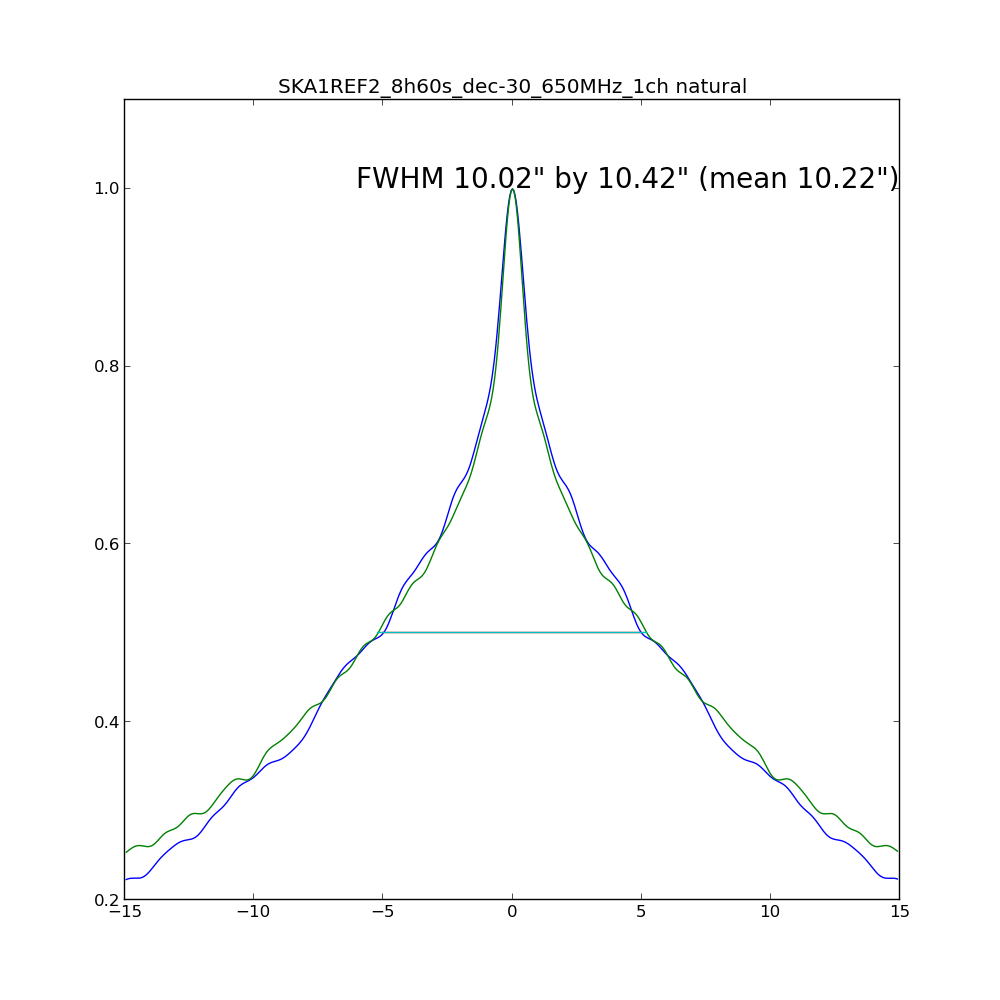
\includegraphics[width=0.180000\textwidth,trim= 0 .05cm 0 0.05cm]{{images/SKA1REF2_8h60s_dec-30_650MHz_1ch-natural-psf.fits}.png} &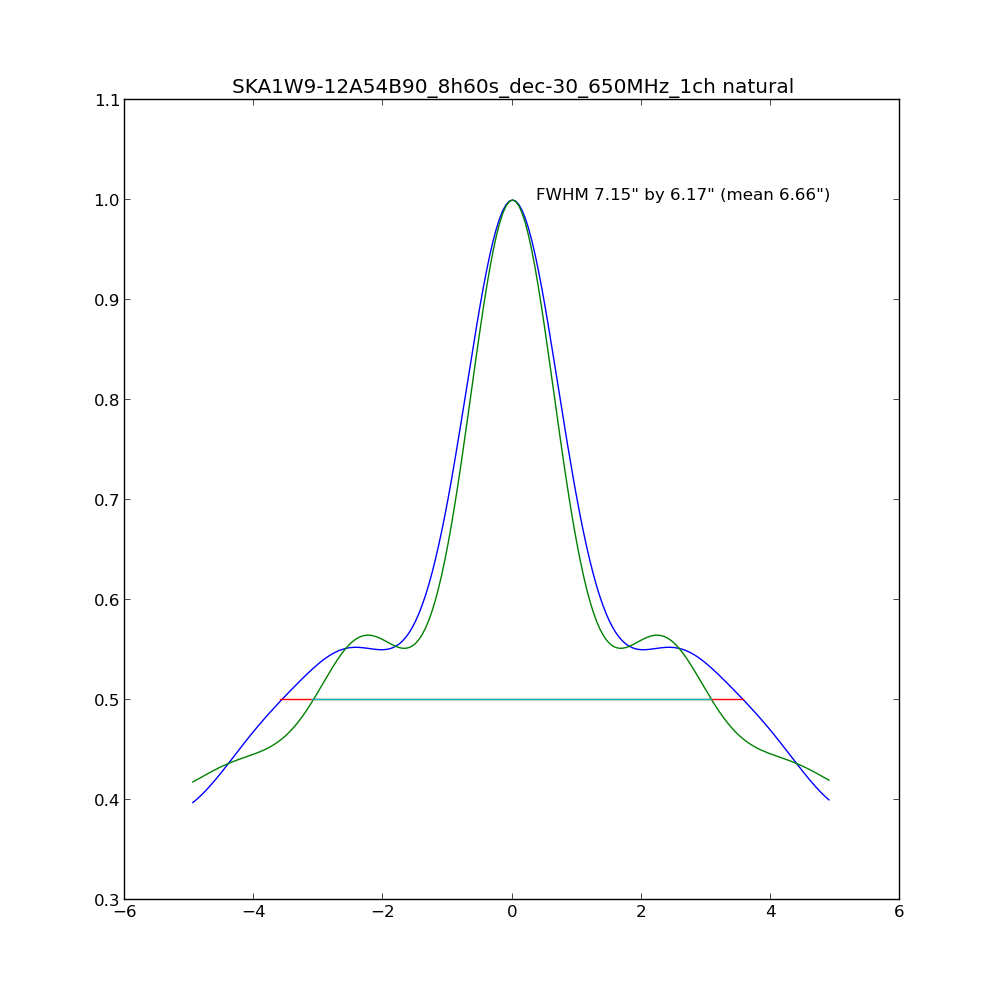
\includegraphics[width=0.180000\textwidth,trim= 0 .05cm 0 0.05cm]{{images/SKA1W9-12A54B90_8h60s_dec-30_650MHz_1ch-natural-psf.fits}.png} &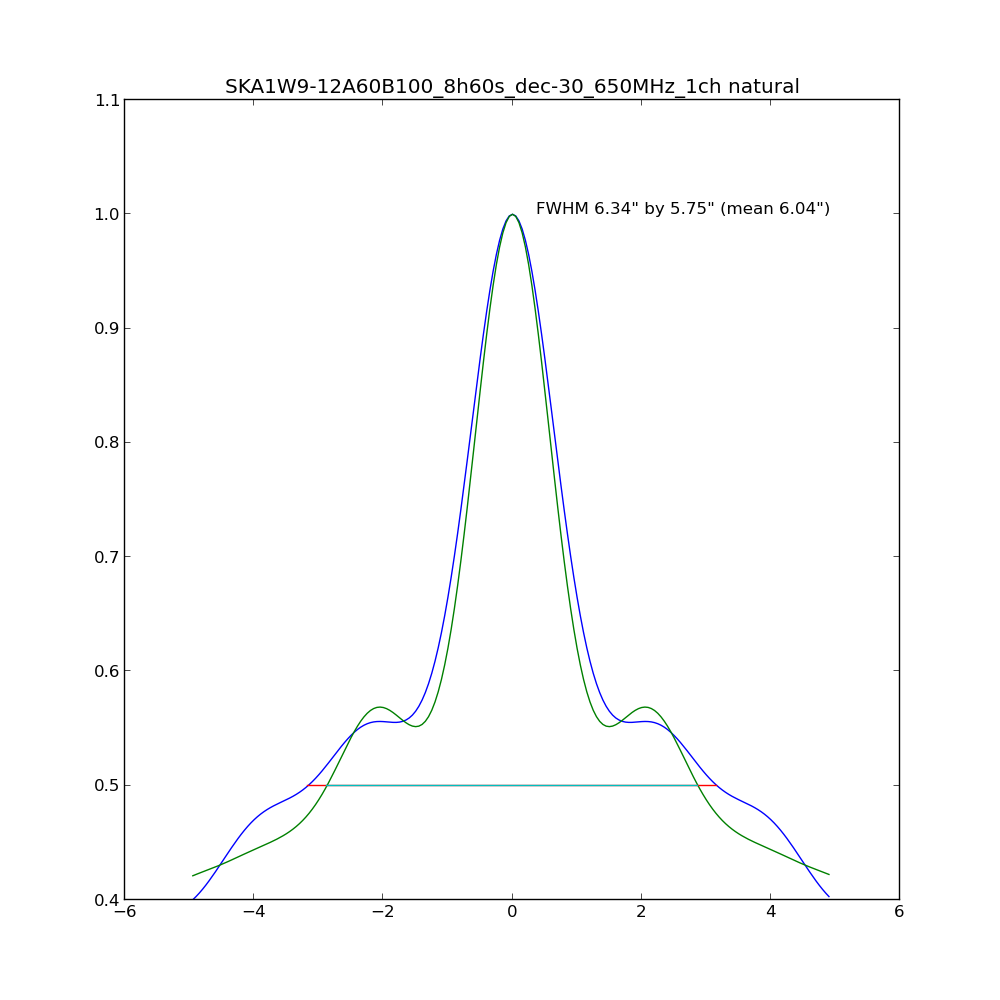
\includegraphics[width=0.180000\textwidth,trim= 0 .05cm 0 0.05cm]{{images/SKA1W9-12A60B100_8h60s_dec-30_650MHz_1ch-natural-psf.fits}.png} &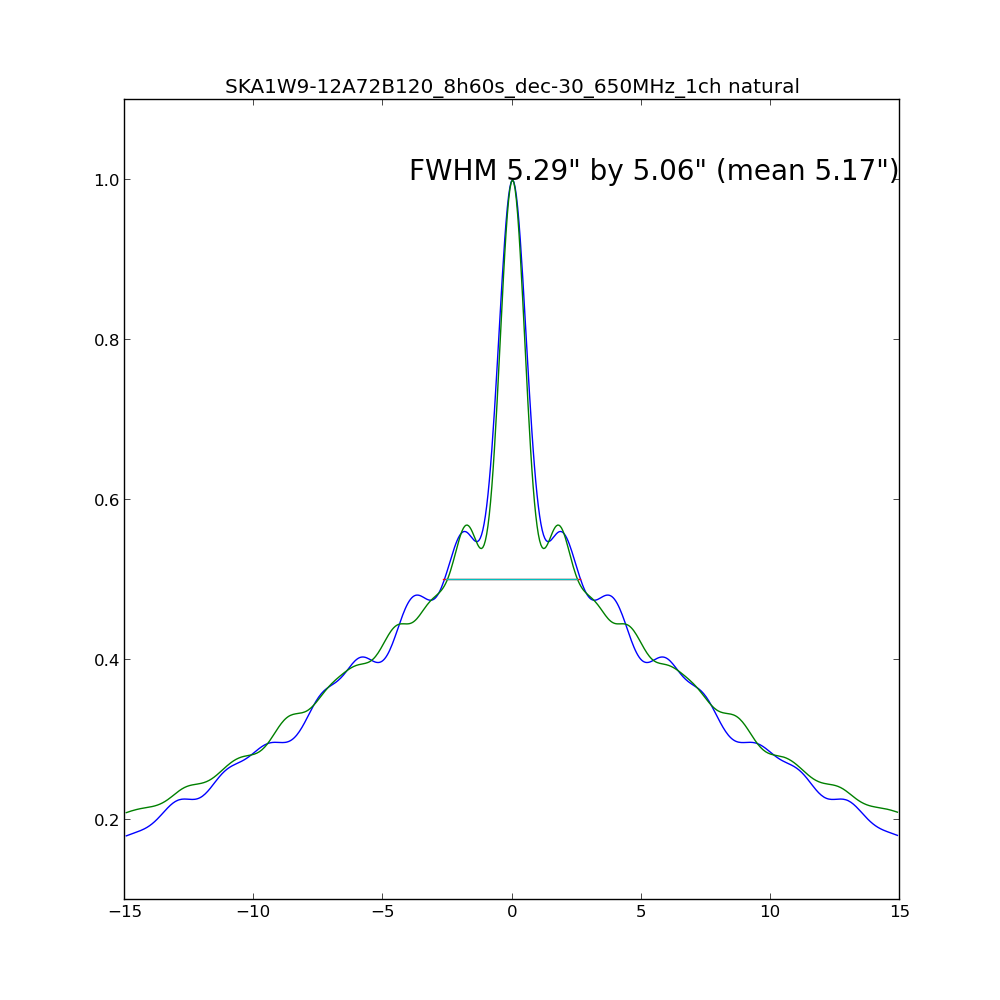
\includegraphics[width=0.180000\textwidth,trim= 0 .05cm 0 0.05cm]{{images/SKA1W9-12A72B120_8h60s_dec-30_650MHz_1ch-natural-psf.fits}.png} &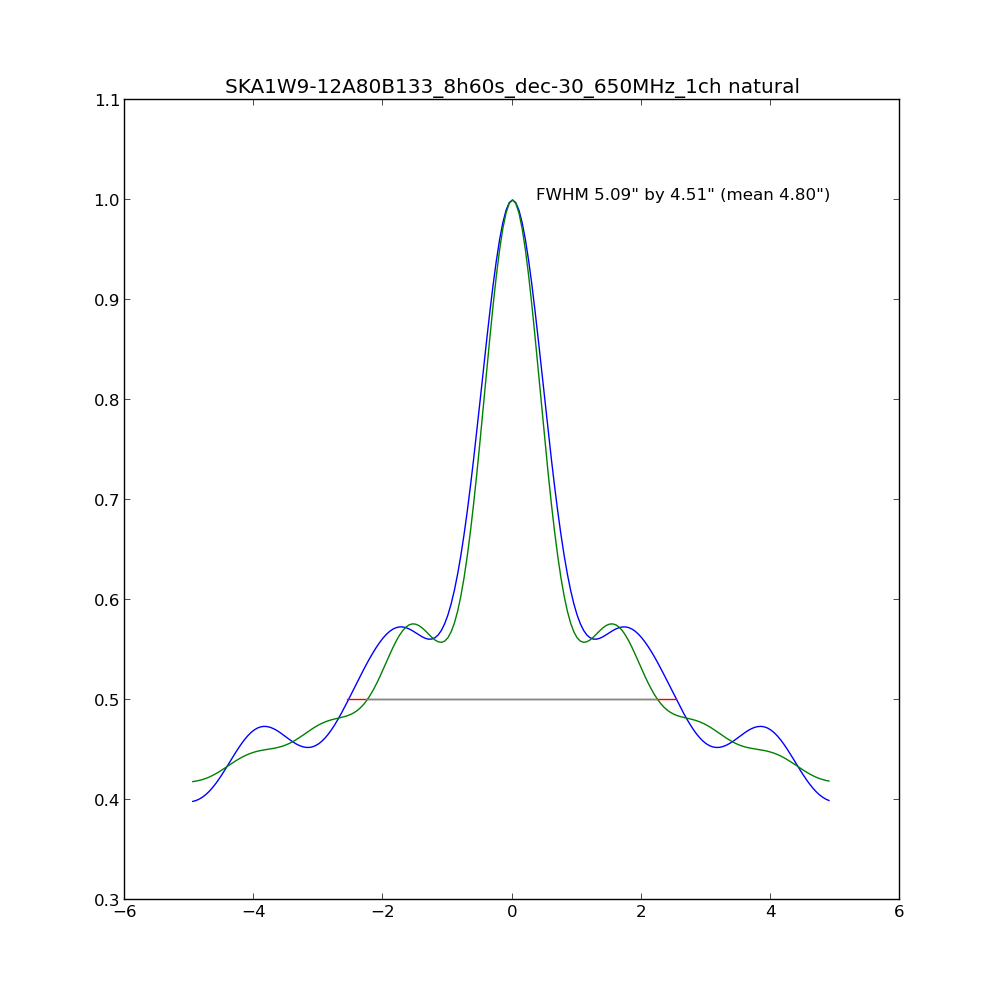
\includegraphics[width=0.180000\textwidth,trim= 0 .05cm 0 0.05cm]{{images/SKA1W9-12A80B133_8h60s_dec-30_650MHz_1ch-natural-psf.fits}.png} \\
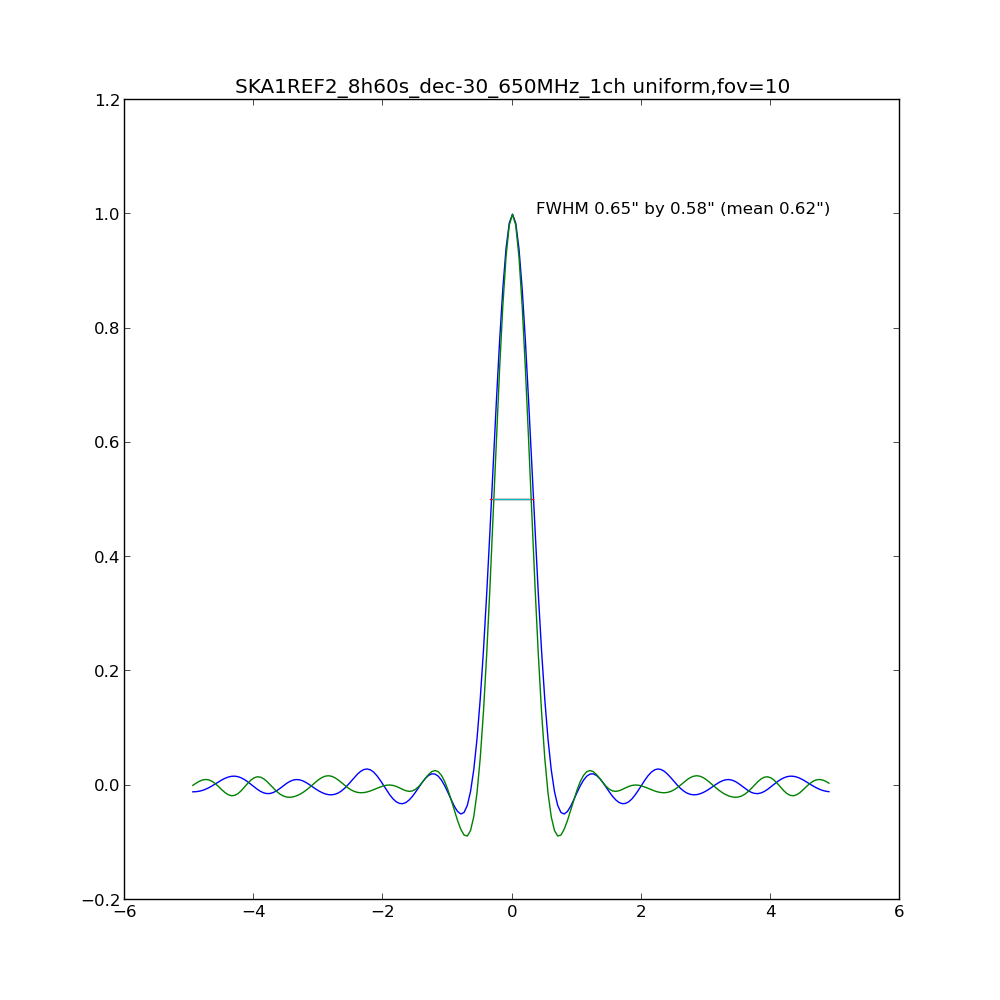
\includegraphics[width=0.180000\textwidth,trim= 0 .05cm 0 0.05cm]{{images/SKA1REF2_8h60s_dec-30_650MHz_1ch-uniform,fov=10-psf.fits}.png} &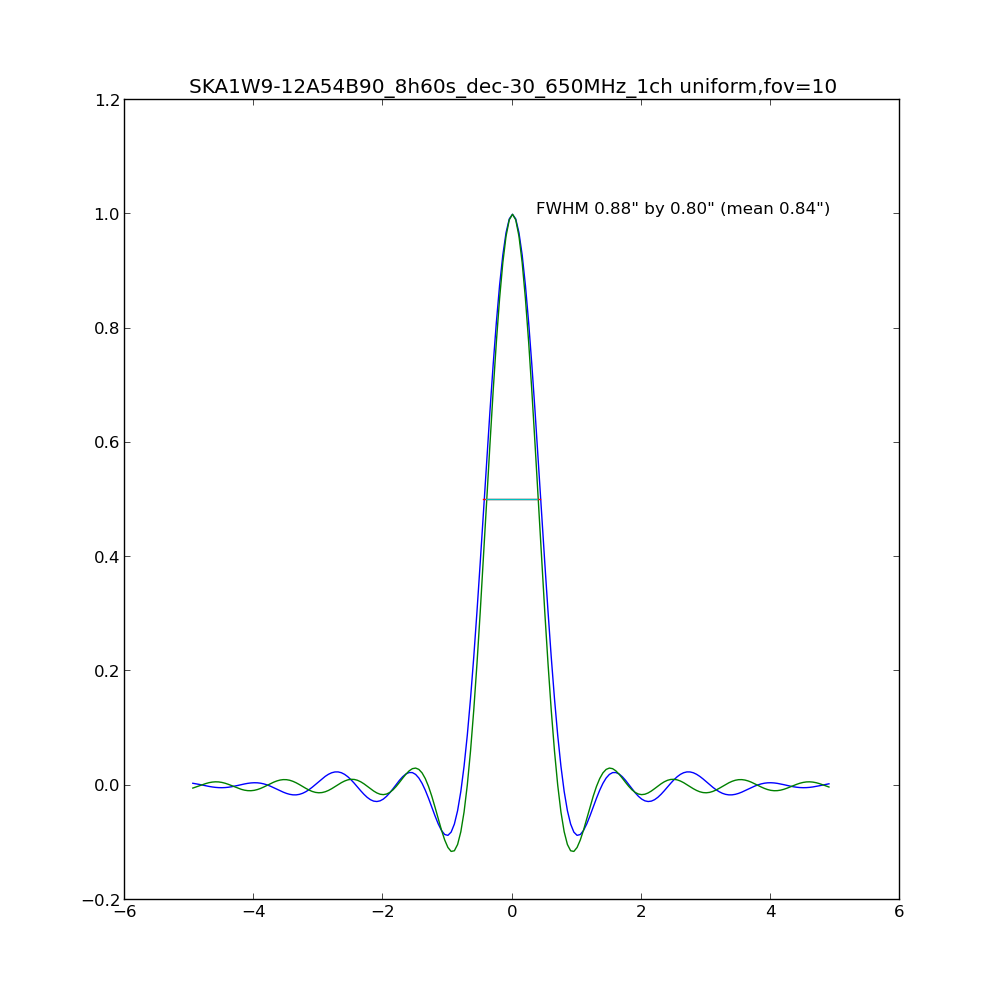
\includegraphics[width=0.180000\textwidth,trim= 0 .05cm 0 0.05cm]{{images/SKA1W9-12A54B90_8h60s_dec-30_650MHz_1ch-uniform,fov=10-psf.fits}.png} &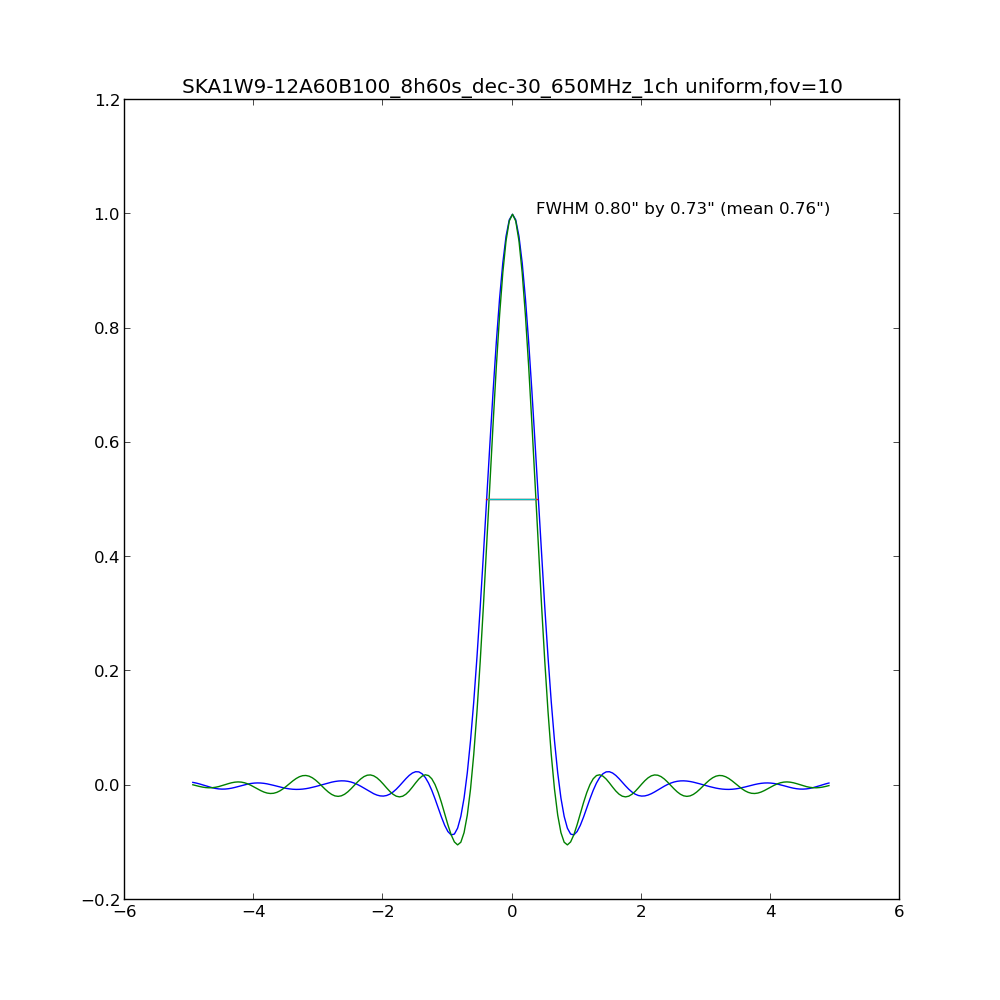
\includegraphics[width=0.180000\textwidth,trim= 0 .05cm 0 0.05cm]{{images/SKA1W9-12A60B100_8h60s_dec-30_650MHz_1ch-uniform,fov=10-psf.fits}.png} &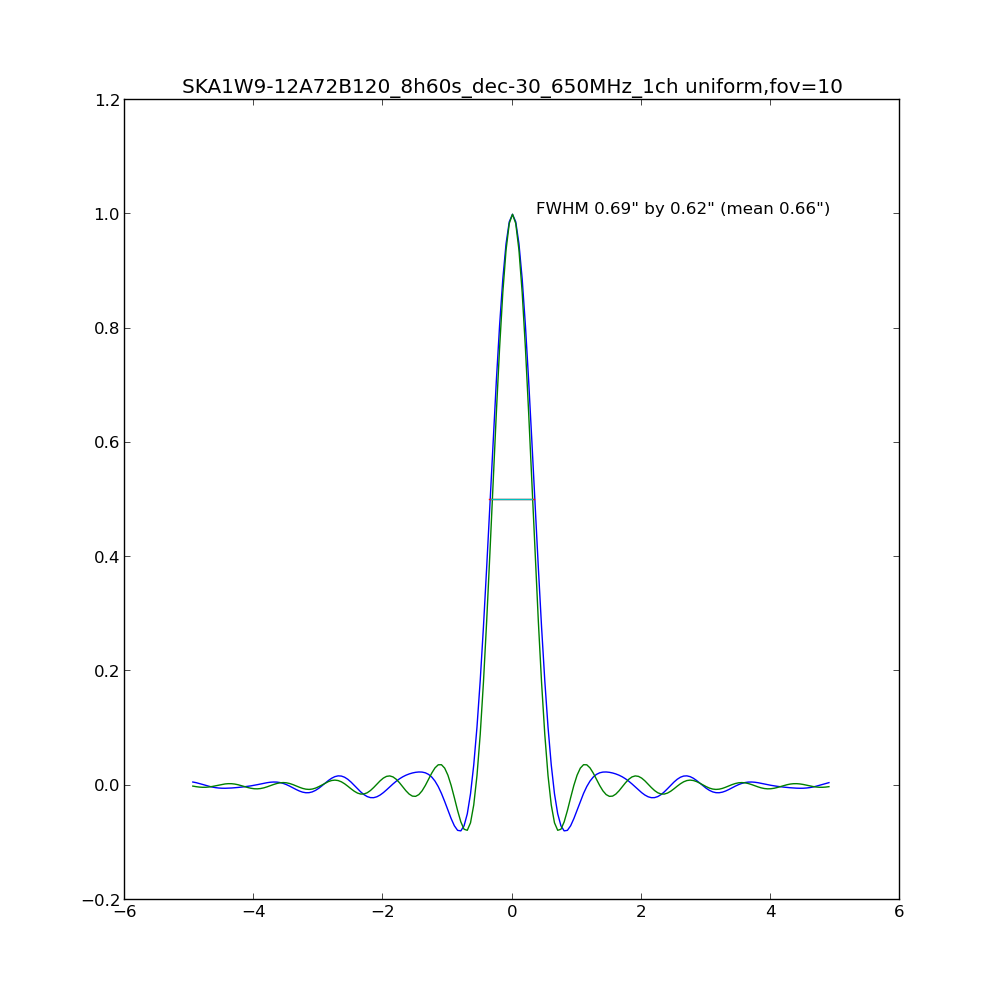
\includegraphics[width=0.180000\textwidth,trim= 0 .05cm 0 0.05cm]{{images/SKA1W9-12A72B120_8h60s_dec-30_650MHz_1ch-uniform,fov=10-psf.fits}.png} &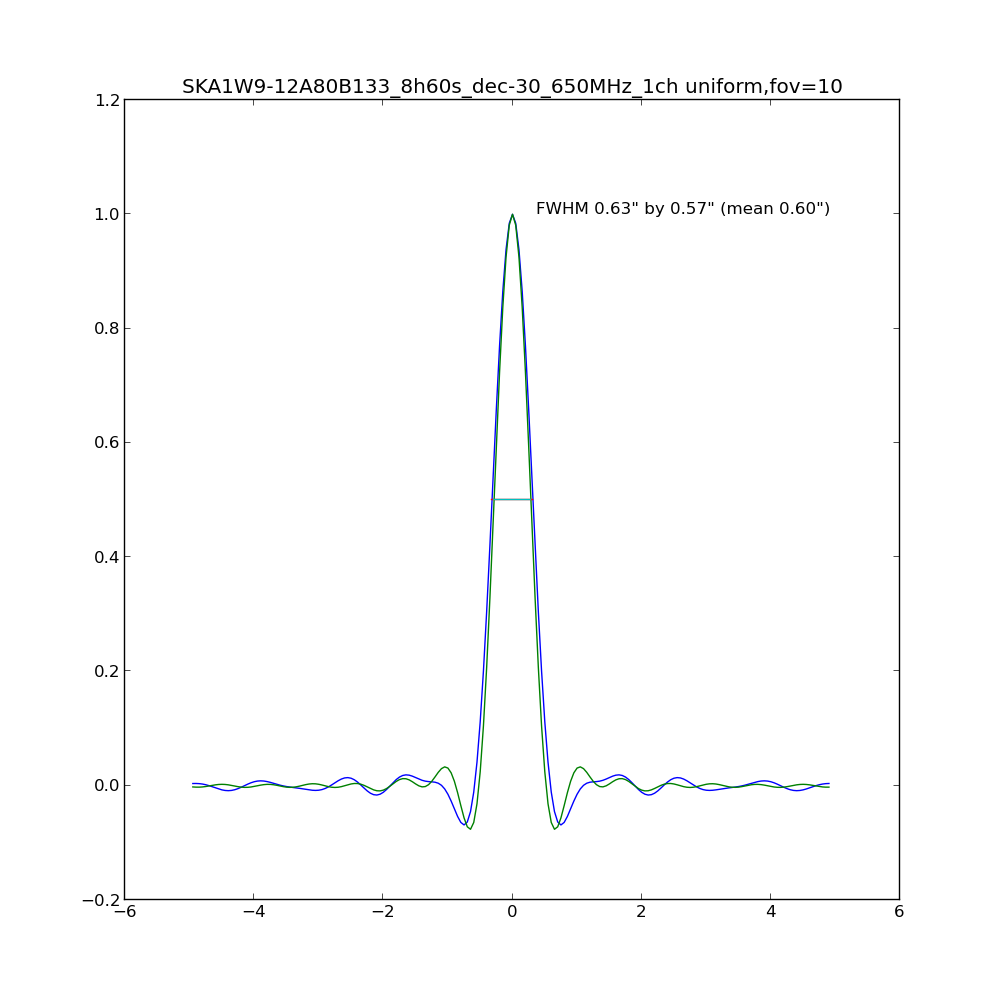
\includegraphics[width=0.180000\textwidth,trim= 0 .05cm 0 0.05cm]{{images/SKA1W9-12A80B133_8h60s_dec-30_650MHz_1ch-uniform,fov=10-psf.fits}.png} \\
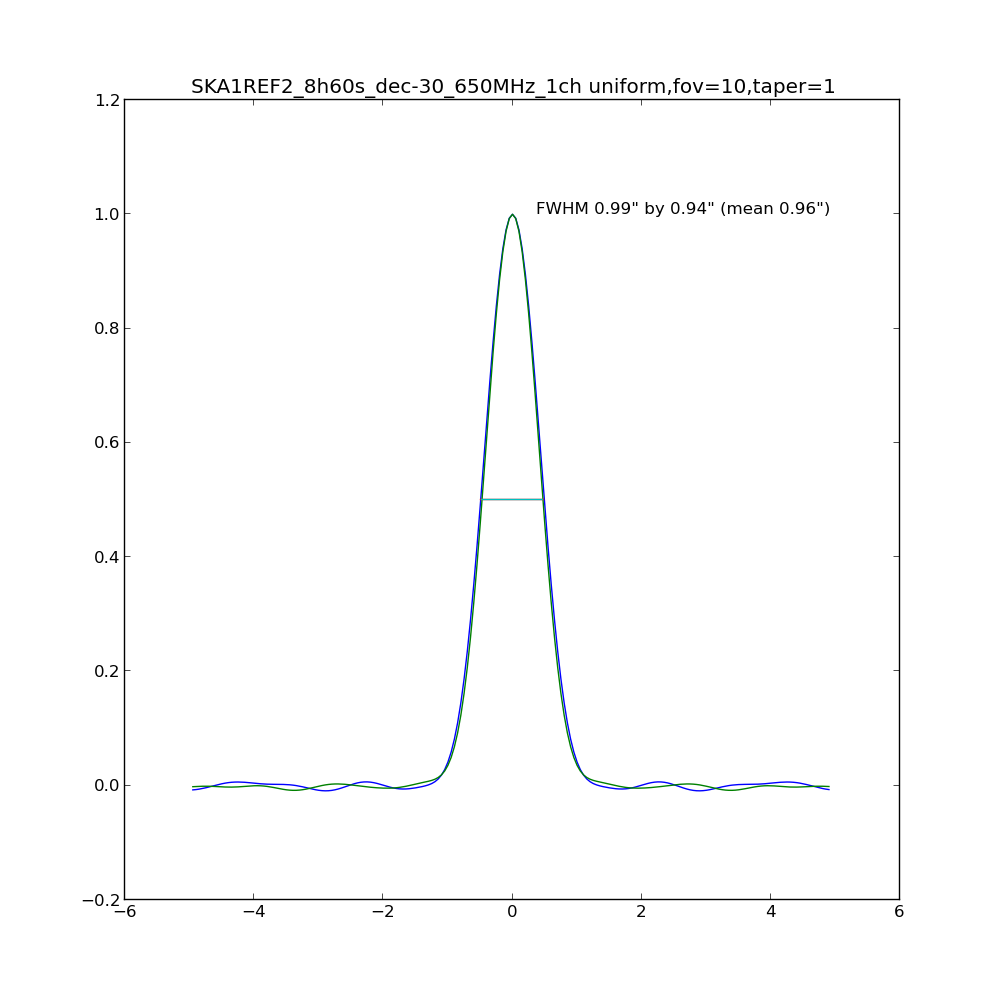
\includegraphics[width=0.180000\textwidth,trim= 0 .05cm 0 0.05cm]{{images/SKA1REF2_8h60s_dec-30_650MHz_1ch-uniform,fov=10,taper=1-psf.fits}.png} &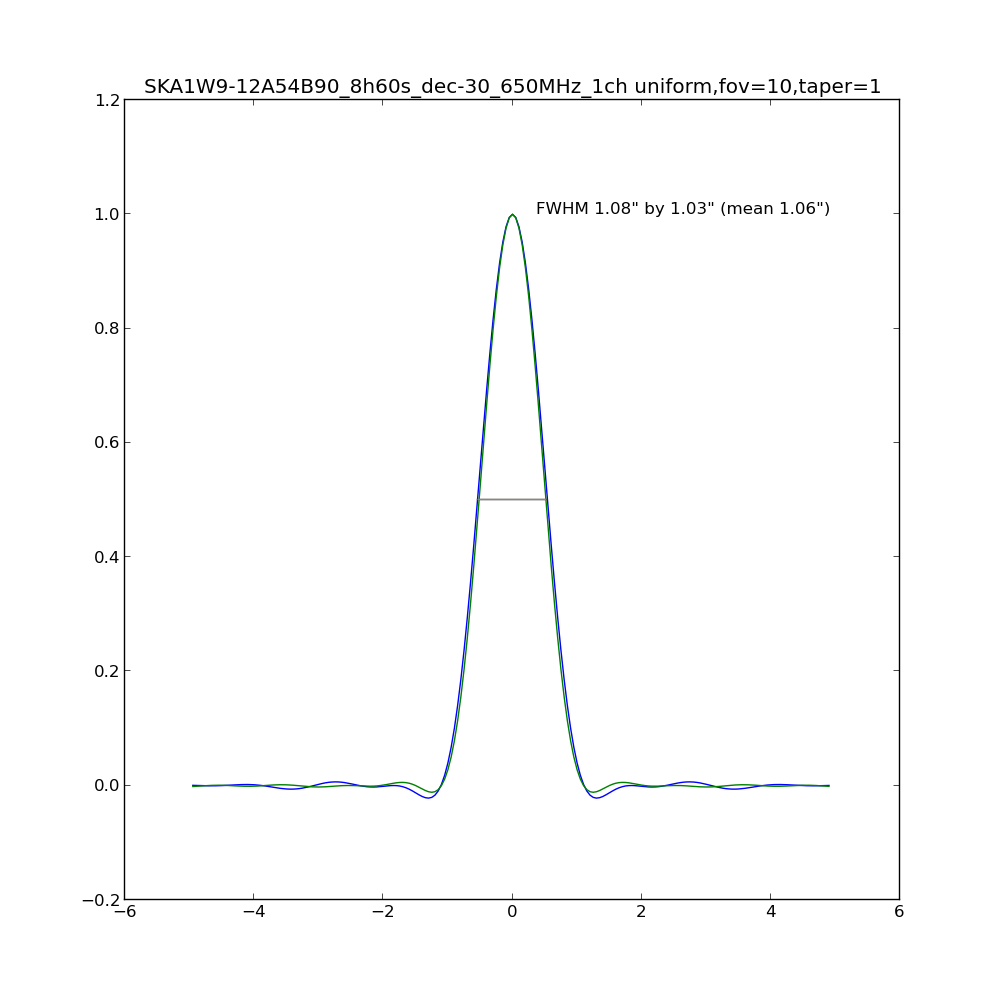
\includegraphics[width=0.180000\textwidth,trim= 0 .05cm 0 0.05cm]{{images/SKA1W9-12A54B90_8h60s_dec-30_650MHz_1ch-uniform,fov=10,taper=1-psf.fits}.png} &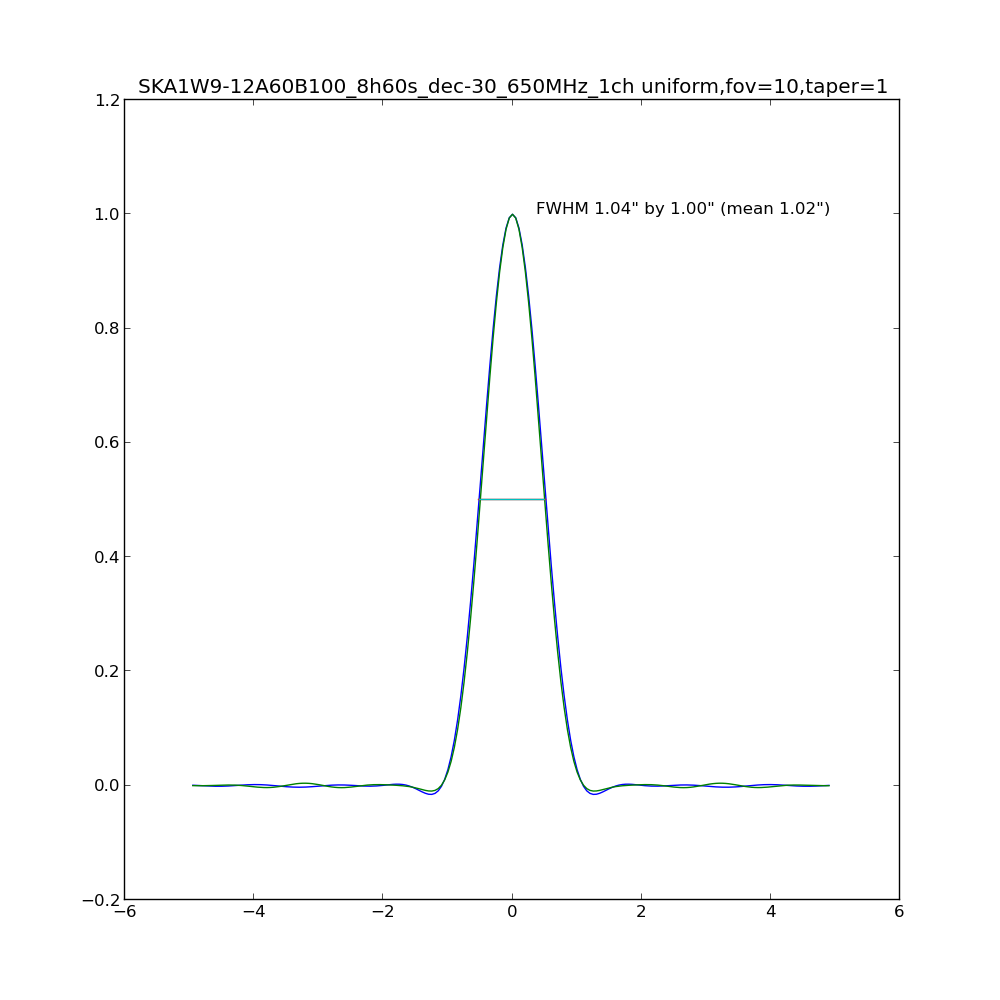
\includegraphics[width=0.180000\textwidth,trim= 0 .05cm 0 0.05cm]{{images/SKA1W9-12A60B100_8h60s_dec-30_650MHz_1ch-uniform,fov=10,taper=1-psf.fits}.png} &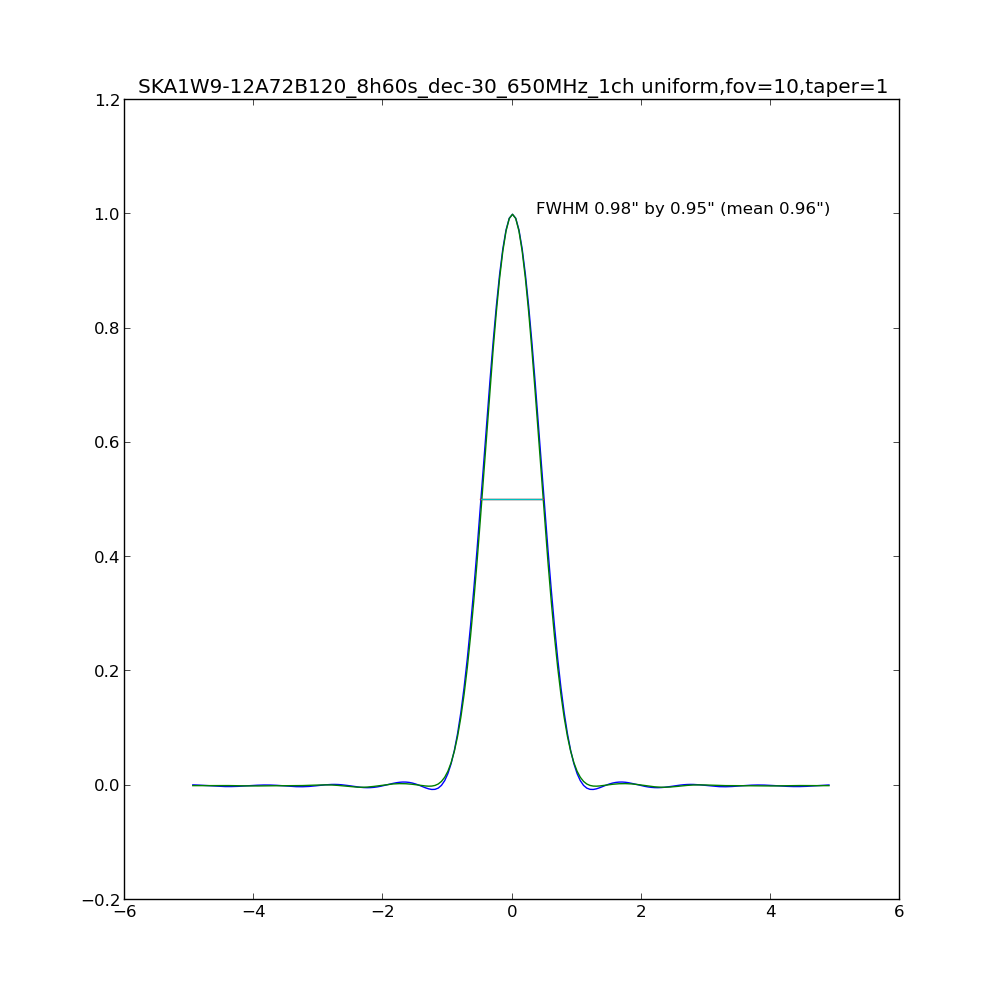
\includegraphics[width=0.180000\textwidth,trim= 0 .05cm 0 0.05cm]{{images/SKA1W9-12A72B120_8h60s_dec-30_650MHz_1ch-uniform,fov=10,taper=1-psf.fits}.png} &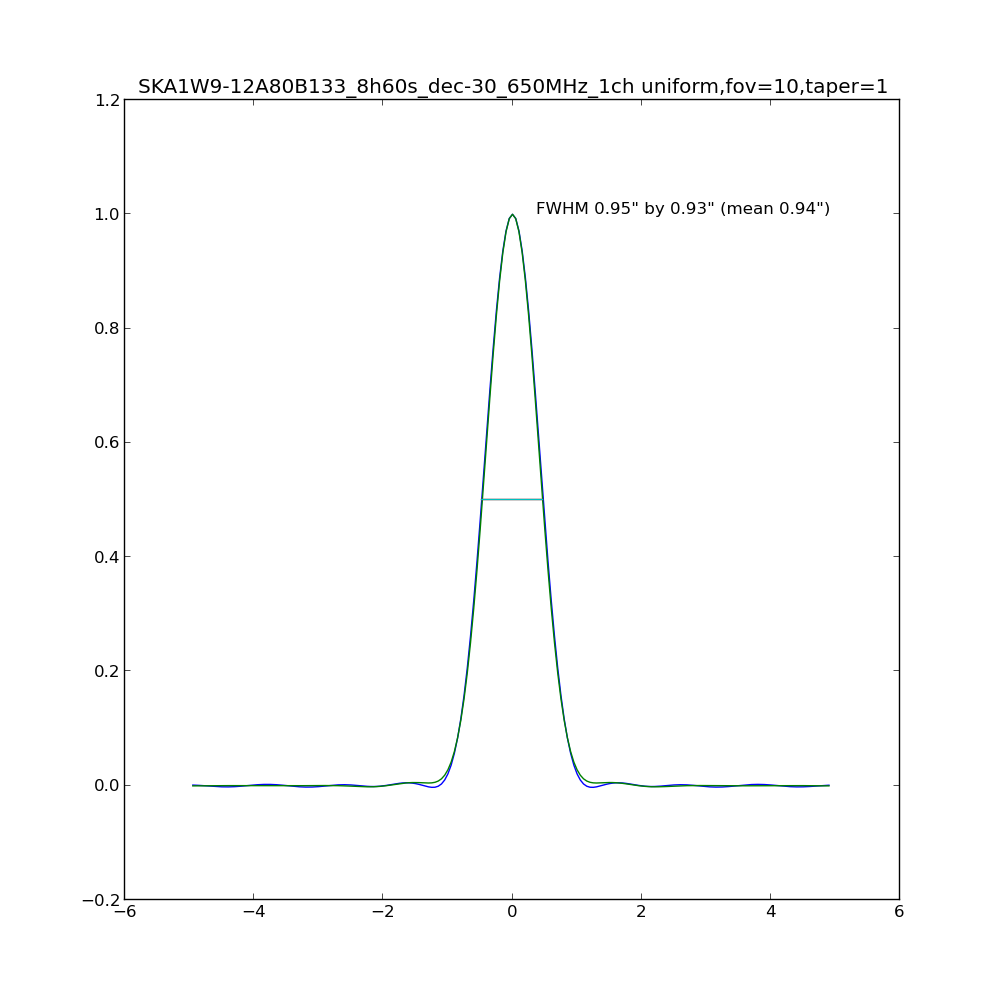
\includegraphics[width=0.180000\textwidth,trim= 0 .05cm 0 0.05cm]{{images/SKA1W9-12A80B133_8h60s_dec-30_650MHz_1ch-uniform,fov=10,taper=1-psf.fits}.png} 
\end{tabular}}
 \caption{PSF cross-sections at Dec=-30 deg, Freq=650MHz. Row 1 and 2 are for natural and robust-2 weighting respectively, and row
3 is for robust-2 weighting with a 1 arcsec Gaussian taper. The blue and green curves are cross-sections along $l$ and $m$
respectively, and the horizontal line marks the FWHM. FWHM parameters are included in the plot. The naturally weighted REF2 PSF
(top left) is larger than 10 arcsec.}
\end{figure}
\begin{figure}[H]
 \tiny{%%% autogen
 \begin{tabular}{ccc}
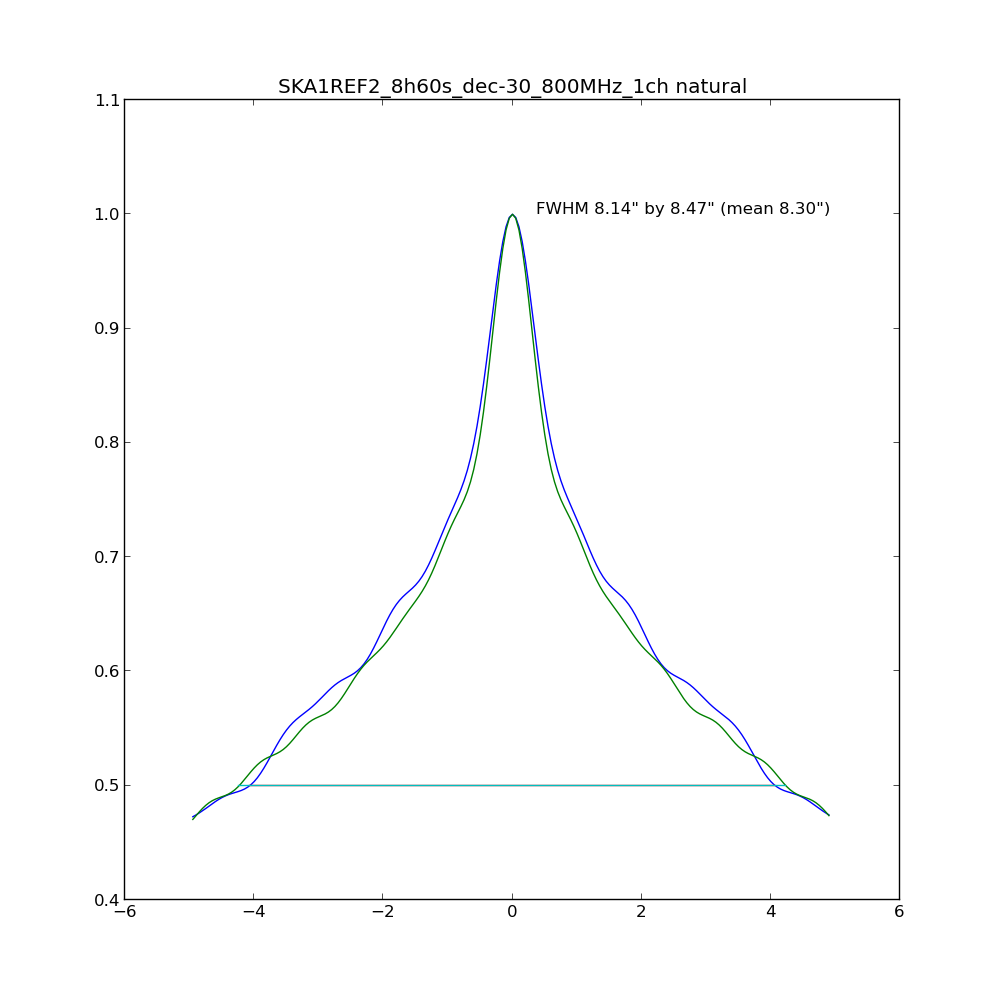
\includegraphics[width=0.300000\textwidth,trim= 0 .05cm 0 0.05cm]{{images/SKA1REF2_8h60s_dec-30_800MHz_1ch-natural-psf.fits}.png} &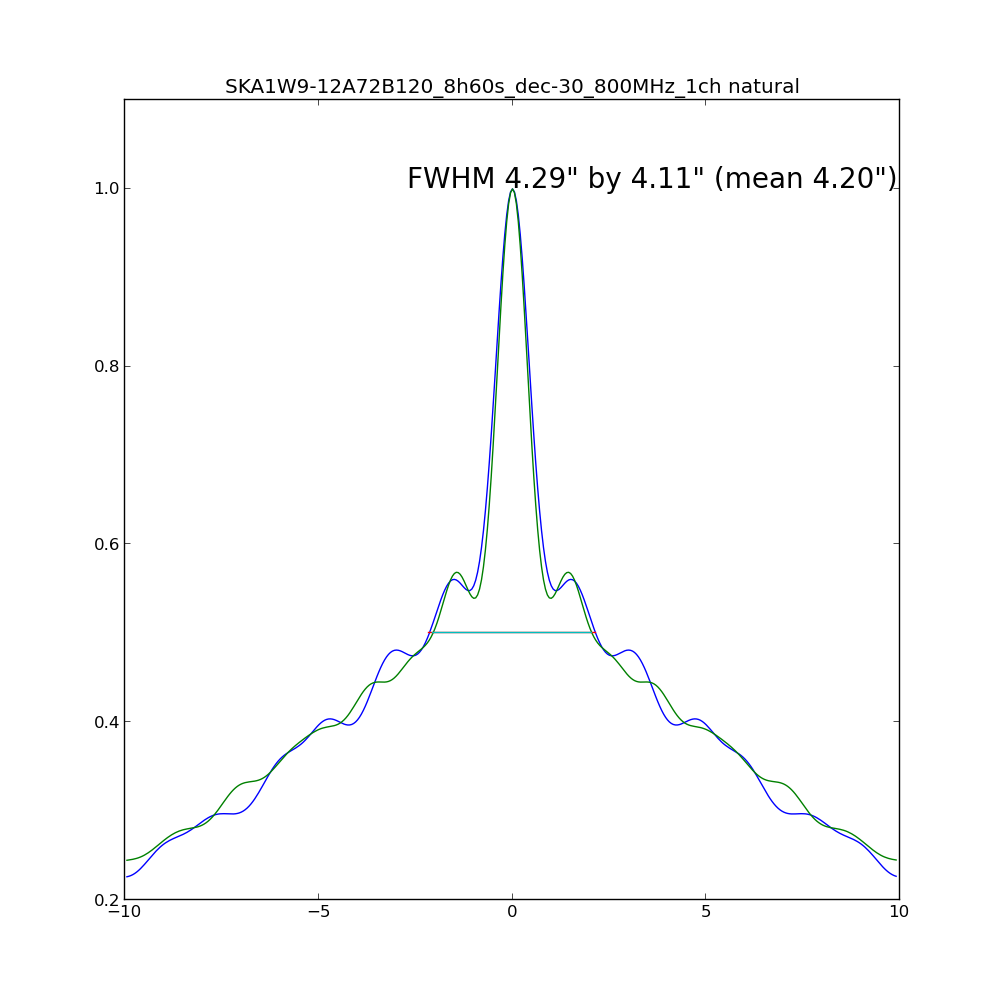
\includegraphics[width=0.300000\textwidth,trim= 0 .05cm 0 0.05cm]{{images/SKA1W9-12A72B120_8h60s_dec-30_800MHz_1ch-natural-psf.fits}.png} &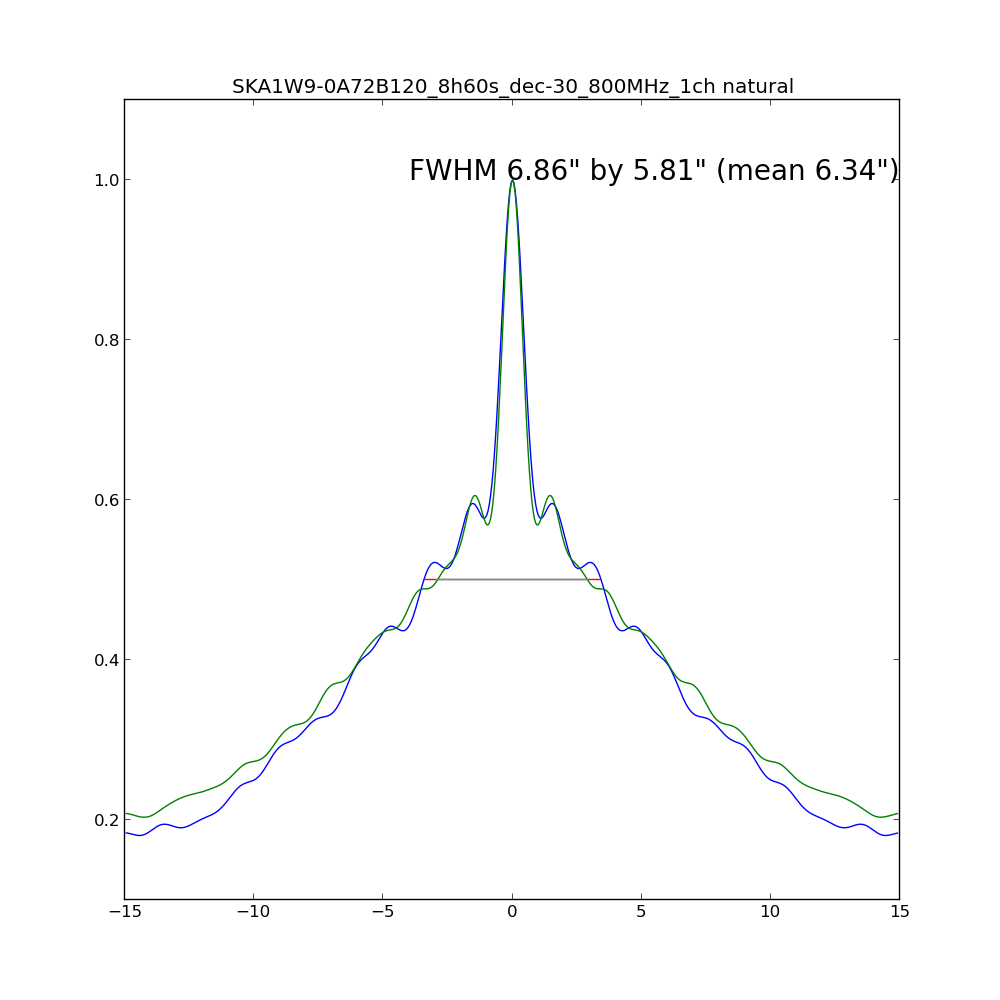
\includegraphics[width=0.300000\textwidth,trim= 0 .05cm 0 0.05cm]{{images/SKA1W9-0A72B120_8h60s_dec-30_800MHz_1ch-natural-psf.fits}.png} 
 \\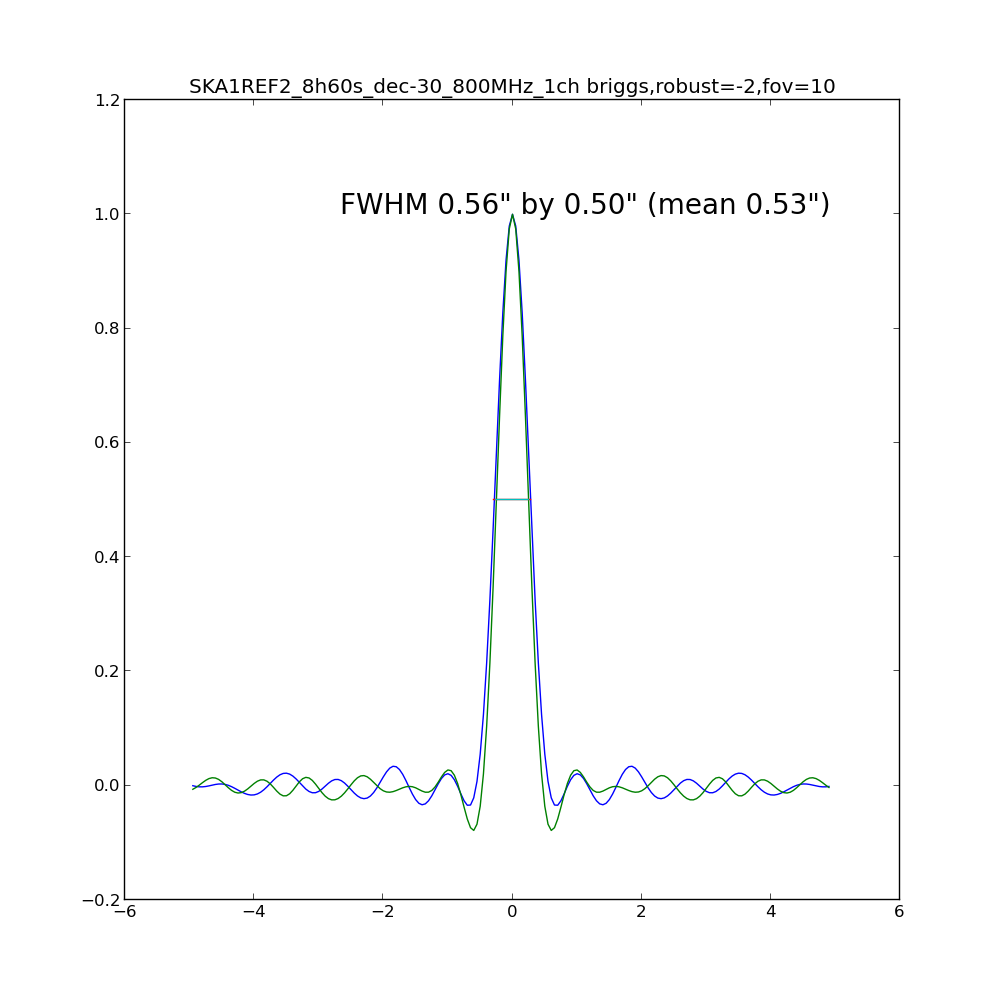
\includegraphics[width=0.300000\textwidth,trim= 0 .05cm 0 0.05cm]{{images/SKA1REF2_8h60s_dec-30_800MHz_1ch-briggs,robust=-2,fov=10-psf.fits}.png} &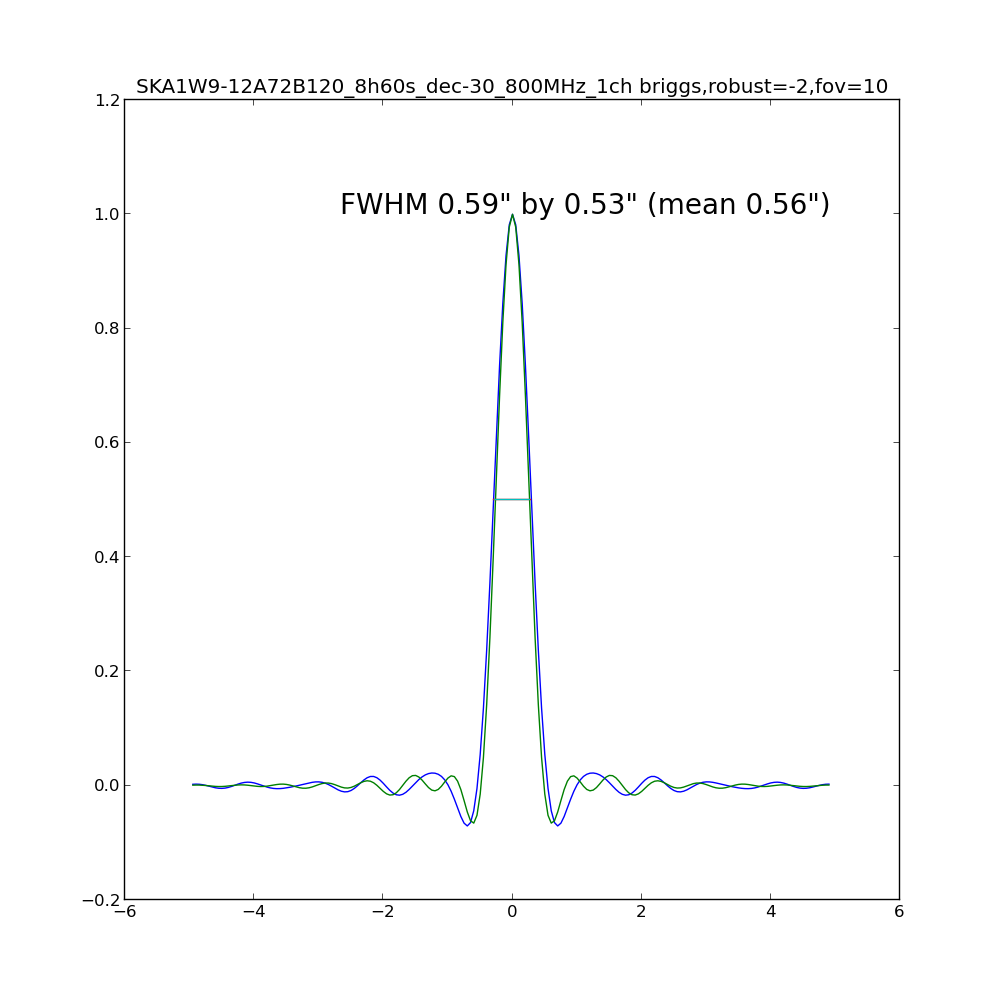
\includegraphics[width=0.300000\textwidth,trim= 0 .05cm 0 0.05cm]{{images/SKA1W9-12A72B120_8h60s_dec-30_800MHz_1ch-briggs,robust=-2,fov=10-psf.fits}.png} &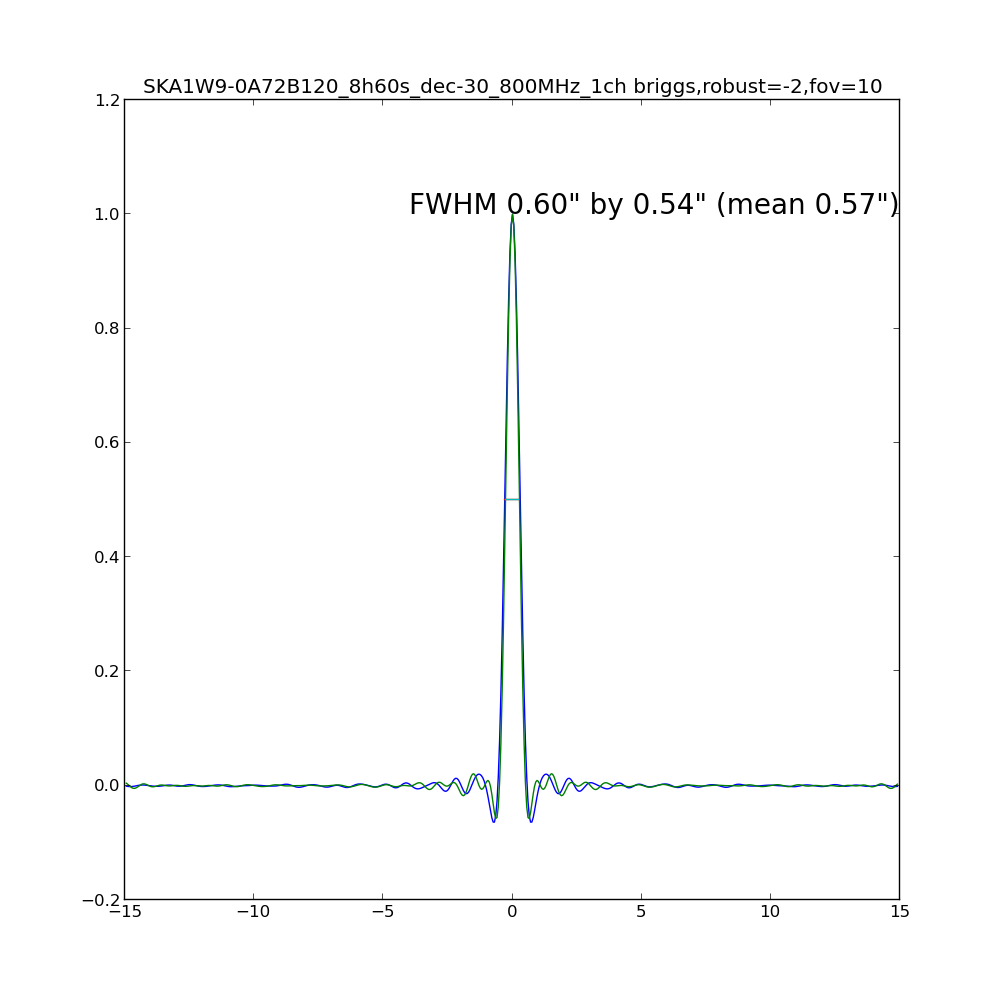
\includegraphics[width=0.300000\textwidth,trim= 0 .05cm 0 0.05cm]{{images/SKA1W9-0A72B120_8h60s_dec-30_800MHz_1ch-briggs,robust=-2,fov=10-psf.fits}.png} 
 \\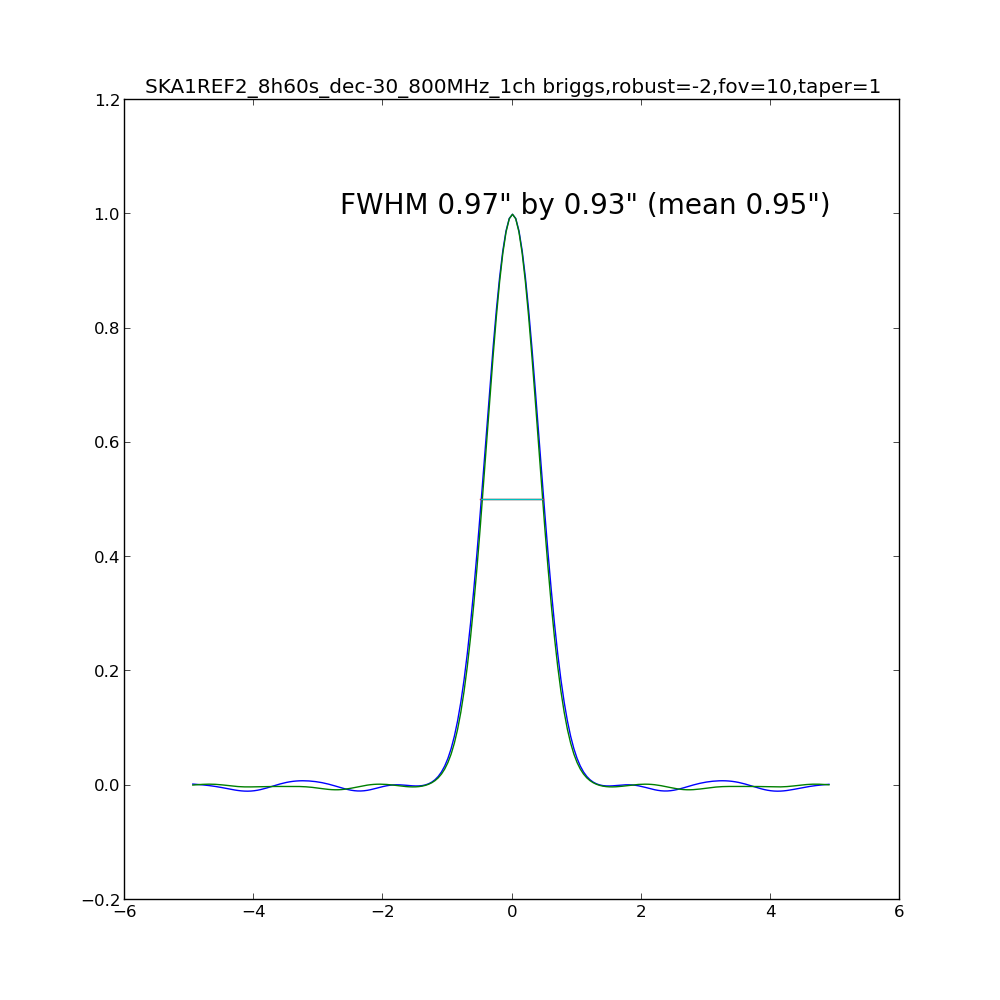
\includegraphics[width=0.300000\textwidth,trim= 0 .05cm 0 0.05cm]{{images/SKA1REF2_8h60s_dec-30_800MHz_1ch-briggs,robust=-2,fov=10,taper=1-psf.fits}.png} &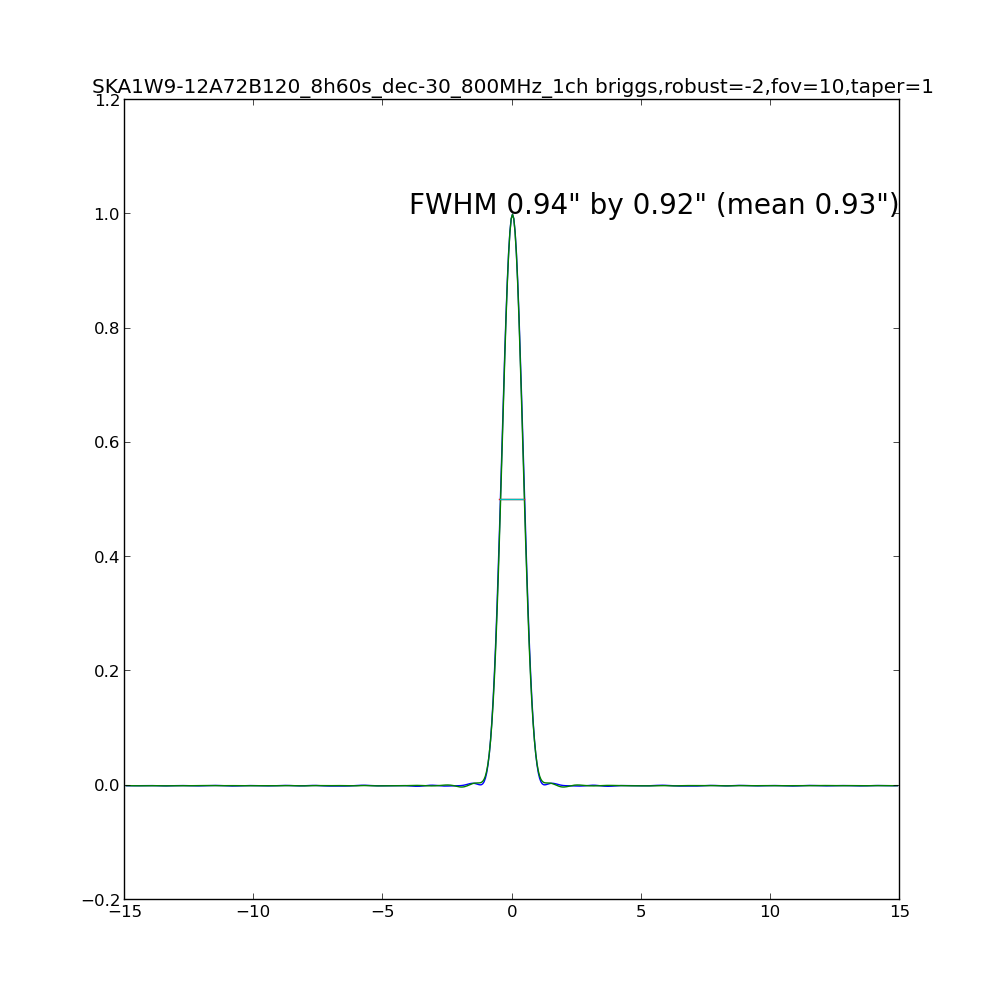
\includegraphics[width=0.300000\textwidth,trim= 0 .05cm 0 0.05cm]{{images/SKA1W9-12A72B120_8h60s_dec-30_800MHz_1ch-briggs,robust=-2,fov=10,taper=1-psf.fits}.png} &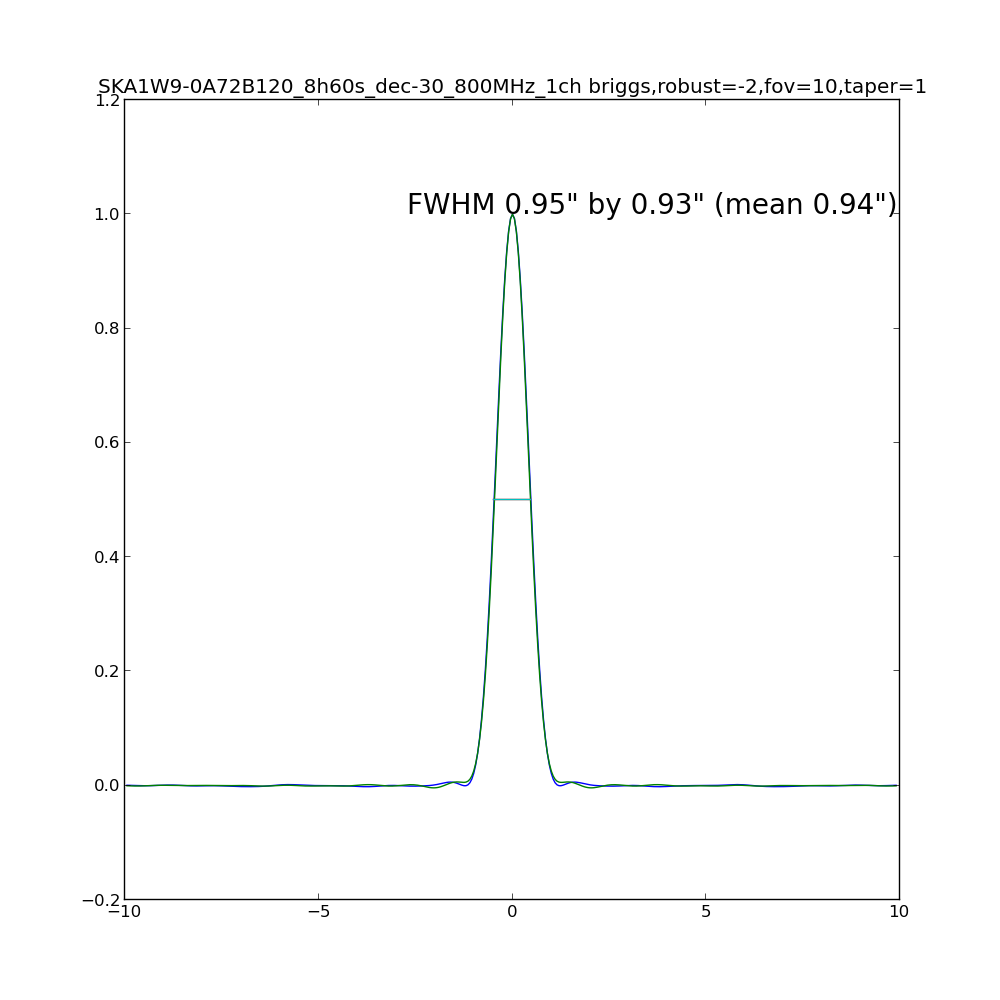
\includegraphics[width=0.300000\textwidth,trim= 0 .05cm 0 0.05cm]{{images/SKA1W9-0A72B120_8h60s_dec-30_800MHz_1ch-briggs,robust=-2,fov=10,taper=1-psf.fits}.png} 
 \\\end{tabular}}
 \caption{PSF cross-sections at Dec=-30 deg, Freq=800MHz. Row 1 and 2 are for natural and robust-2 weighting respectively, and 
row
3 is for robust-2 weighting with a 1 arcsec Gaussian taper. The blue and green curves are cross-sections along $l$ and $m$
respectively, and the horizontal line marks the FWHM. FWHM parameters are included in the plot.}
\end{figure}
\begin{figure}[H]
 \tiny{%%% autogen
 \begin{tabular}{ccc}
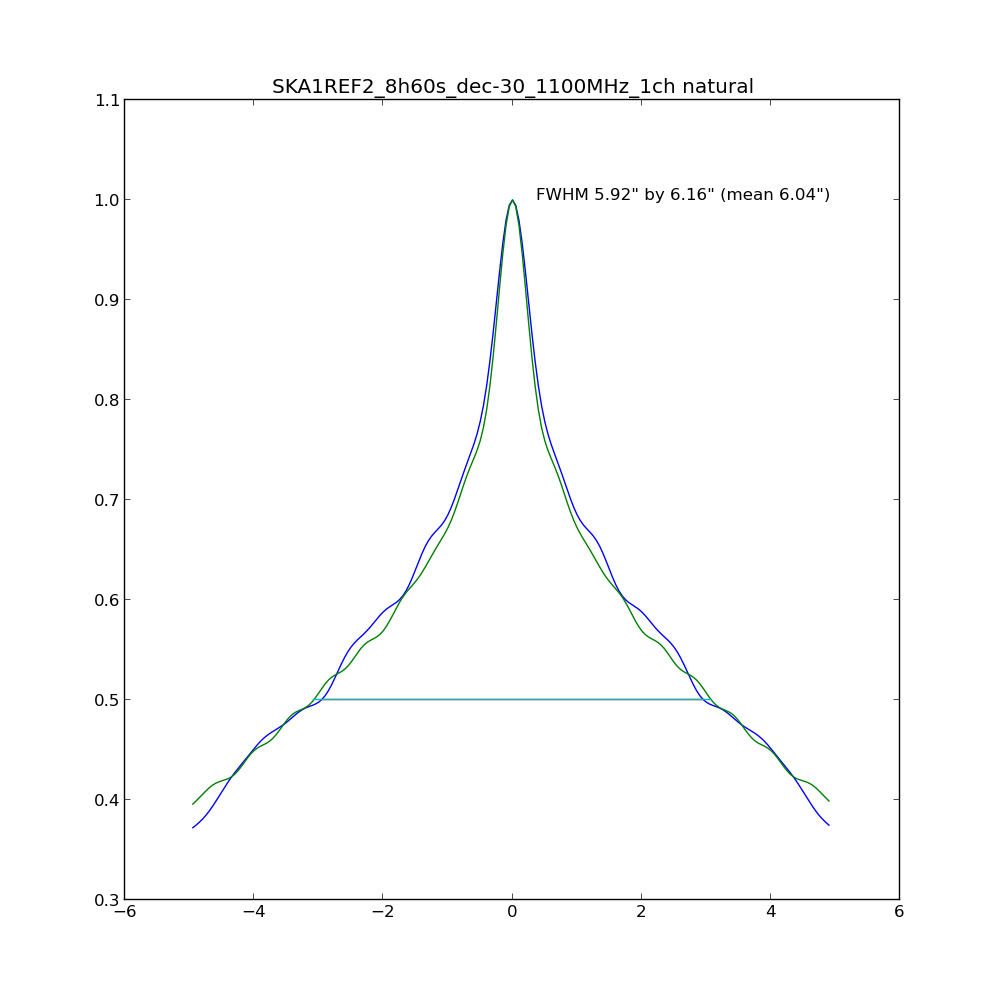
\includegraphics[width=0.300000\textwidth,trim= 0 .05cm 0 0.05cm]{{images/SKA1REF2_8h60s_dec-30_1100MHz_1ch-natural-psf.fits}.png} &\includegraphics[width=0.300000\textwidth,trim= 0 .05cm 0 0.05cm]{{images/SKA1W9-12A72B120_8h60s_dec-30_1100MHz_1ch-natural-psf.fits}.png} &\includegraphics[width=0.300000\textwidth,trim= 0 .05cm 0 0.05cm]{{images/SKA1W9-0A72B120_8h60s_dec-30_1100MHz_1ch-natural-psf.fits}.png} 
 \\\includegraphics[width=0.300000\textwidth,trim= 0 .05cm 0 0.05cm]{{images/SKA1REF2_8h60s_dec-30_1100MHz_1ch-briggs,robust=-2,fov=10-psf.fits}.png} &\includegraphics[width=0.300000\textwidth,trim= 0 .05cm 0 0.05cm]{{images/SKA1W9-12A72B120_8h60s_dec-30_1100MHz_1ch-briggs,robust=-2,fov=10-psf.fits}.png} &\includegraphics[width=0.300000\textwidth,trim= 0 .05cm 0 0.05cm]{{images/SKA1W9-0A72B120_8h60s_dec-30_1100MHz_1ch-briggs,robust=-2,fov=10-psf.fits}.png} 
 \\\includegraphics[width=0.300000\textwidth,trim= 0 .05cm 0 0.05cm]{{images/SKA1REF2_8h60s_dec-30_1100MHz_1ch-briggs,robust=-2,fov=10,taper=1-psf.fits}.png} &\includegraphics[width=0.300000\textwidth,trim= 0 .05cm 0 0.05cm]{{images/SKA1W9-12A72B120_8h60s_dec-30_1100MHz_1ch-briggs,robust=-2,fov=10,taper=1-psf.fits}.png} &\includegraphics[width=0.300000\textwidth,trim= 0 .05cm 0 0.05cm]{{images/SKA1W9-0A72B120_8h60s_dec-30_1100MHz_1ch-briggs,robust=-2,fov=10,taper=1-psf.fits}.png} 
 \\\end{tabular}}
 \caption{PSF cross-sections at Dec=-30 deg, Freq=1100MHz. Row 1 and 2 are for natural and robust-2 weighting respectively, and
row
3 is for robust-2 weighting with a 1 arcsec Gaussian taper. The blue and green curves are cross-sections along $l$ and $m$
respectively, and the horizontal line marks the FWHM. FWHM parameters are included in the plot.}
\end{figure}

\end{document}

